%% Copyright (C) 2018 Adrien Blanchet
%%

%%%%%%%%%%%%%%%%%%%%%%%%%%%%%%%%%%%%%%%%
%             Chapitre Stat               %
%%%%%%%%%%%%%%%%%%%%%%%%%%%%%%%%%%%%%%%%

\chapter{Analyse statistique}
\label{chap:chapitre_stat}

\citationChap{
With four parameters I can fit an elephant, and with five I can make him wiggle his trunk.
}{John von Neumann}{A meeting with Enrico Fermi}

\minitoc

\newpage

\section{Principe d'une déduction statistique}

Une déduction statistique, ou inférence statistique est une procédure d'analyse des données qui vise à décider de la pertinence d'une prédiction connaissant les lois de probabilité sous-jacentes. L'approche adoptée ici est \textit{fréquentiste} (aussi appelée \textit{classique}) et la qualité d'un modèle est quantifiée en niveau de confiance (\og C.L. \fg{} pour \textit{Confidence Level}).\\

Une discussion d'un point de vue général et opératoire sur l'inférence statistique est présentée en premier lieu, suivie d'une explication sur l'origine de ce formalisme dans un second temps.

\bigbreak

\subsection{Comparaison des données avec une prédiction}

Une mesure seule ne dit rien sur les processus qui lui ont donné naissance: c'est une réalisation statistique à la suite d'une avalanche de causes à effets. En ce sens une mesure n'a pas d'erreur, sa nature n'est qu'une suite de chiffres bruts sans signification. En fait, l'estimation des erreurs associées à l'instrumentation est une croyance, une prédiction sur le comportement hypothétique de la répétition de cette mesure. Ces erreurs représentent donc une plage autour d'une \og valeur vraie \fg{}, dans laquelle les mesures, c'est-à-dire les réalisations statistiques, se distribuent. À notre grand désespoir, cette valeur vraie n'est pas connue, c'est justement l'objet de notre quête. Il est en revanche possible d'émettre des hypothèses par le biais de modèles prédictifs et d'interpréter leur validité en associant à chaque modèle l'incertitude d'une réalisation (mesure) de ce modèle. L'objet de cette discussion est de souligner l'appartenance des erreurs à une prédiction et non aux données mesurées. En effet, d'ordinaire nous entendons associer à tort les erreurs aux mesures, comme dans l'exemple: \og l'erreur statistique sur un taux de comptage est $\sqrt{N}$ où N est le nombre de coups mesurés \fg{}. Cette distinction s'avère particulièrement cruciale dans le cadre d'une analyse statistique sur des motifs d'oscillation, car pour de grands angles de mélange le taux de comptage neutrino prédit est largement réduit et l'erreur statistique doit être adaptée pour interpréter correctement la validité de l'hypothèse.\\

% À notre grand désespoir cette valeur vraie n'est pas connue, et comme le disait Albert Camus: la \og \textit{vérité est mystérieuse, fuyante, toujours à conquérir} \fg{}; autrement dit cette valeur est l'objet de notre quête.

Dans cette analyse, l'écart entre $N$ mesures indépendantes et $N$ prédictions est quantifié à l'aide d'une statistique dénommée $\chi^2$ dont la forme sera justifiée dans la section suivante:

\begin{equation}
\label{eq:basic_chi2}
    \chi^2 = \sum_i^\textrm{N mesures} \left( \frac{D_i - M_i}{\sigma_i} \right)^2,
\end{equation}

\bigbreak

où $D_i$ représente les données mesurées, $M_i$ le modèle à tester, et $\sigma_i$ l'écart type \textbf{associé à la prédiction $M_i$}. Si les $M_i$ présentent des corrélations entre elles, $\sigma_i$ est remplacé par une matrice de covariance:

\begin{equation}
\label{eq:cov_chi2}
    \chi^2 = \sum_i^\textrm{N} \sum_j^\textrm{N} \Delta_i^t \left( V_\textrm{cov}^{-1} \right)_{ij} \Delta_j,
\end{equation}

\bigbreak

avec $\Delta_i \doteq D_i - M_i$ et $V_\textrm{cov}$ la matrice de covariance des $\Delta_i$ (ou $M_i$). Si les donnes $D_i$ sont une réalisation statistique du modèle $M_i$ alors le $\chi^2$ doit suivre une densité de probabilité appelée \og loi normale \fg{} à N degrés de liberté. Ces lois tabulées permettent de déduire le niveau de confiance d'un modèle par rapport au jeu de données mesuré. Le niveau de confiance, aussi appelé parfois \og \textit{p-value} \fg{}, représente la fraction d'expériences issues de la prédiction ($M_i$) ayant un $\chi^2$ plus grand que celui obtenu avec la mesure $D_i$. Notons que si le modèle ne suit pas  une loi normale, les niveaux de confiance sont déduits d'une distribution de $\chi^2$ générée par pseudo-expériences où les données $D_i$ sont des réalisations selon la loi dictée par le modèle.\\

Le formalisme en $\chi^2$ permet également d'inclure des paramètres dits \og de nuisance \fg{} qui affectent la prédiction $M_i$. Les valeurs des paramètres de nuisance sont contraintes par des termes de traction (\og \textit{pull terms} \fg{}) qui délimitent une zone de confiance. Dans ce cas, l'expression du $\chi^2$ devient:

\begin{equation}
\label{eq:nuisance_param_chi2}
    \chi^2 = \sum_i^\textrm{N mesures} \left( \frac{D_i - M_i(\{ \alpha_k \})}{\sigma_i} \right)^2 + \sum_k \left( \frac{\alpha_k}{\sigma_k} \right)^2,
\end{equation}

\bigbreak

où $\alpha_k$ sont les paramètres de nuisances et $\sigma_k$ leur écart type. La minimisation du $\chi^2$ à l'aide des $\alpha_k$ permet d'interpréter à nouveau sa valeur en terme de \textit{p-value}. En pratique ce formalisme est exploité pour traiter les erreurs systématiques. Il est notamment utile pour repérer des biais sur les modèles employés en examinant la valeur des paramètres de nuisance choisis pour minimiser le $\chi^2$. De manière équivalente, le traitement des erreurs systématiques peut être établi par une matrice de covariance globale:

\begin{equation}
    V_\textrm{cov} = V_\textrm{stat} + V_\textrm{syst} = V_\textrm{stat} + \sum_k V_\textrm{syst}^k,
\end{equation}

\bigbreak

avec $V_\textrm{syst}$ la somme des matrices de covariance associée à chaque composante d'erreurs systématiques $V_\textrm{syst}^k$. Cette écriture présente l'avantage de s'affranchir de l'étape de minimisation du $\chi^2$ avec les pull terms qui peut s'avérer très consommatrice de temps de calcul. La matrice $V_\textrm{syst}$ peut être obtenue de deux façons: numériquement ou analytiquement. La méthode numérique consiste à tirer des $\alpha_k$ dans leur gaussienne respective de largeur $\sigma_k$ et de propager leur impact sur la prédiction $M_i$. La matrice est estimée à chaque tirage jusqu'à ce que chaque élément ait convergé:

\begin{equation}
    \left[ V_\textrm{syst} \right]_{ij} = \lim\limits_{N \to +\infty} \sum_n^N \left(M_i(\alpha^n_k) - \frac{\sum_{n'}^N M_i(\alpha^{n'}_k)}{N}\right) \left(M_j(\alpha^n_k) - \frac{\sum_{n'}^N M_j(\alpha^{n'}_k)}{N}\right) \times \frac{1}{N}.
\end{equation}

\bigbreak

D'autre part, il est possible d'obtenir $V_\textrm{syst}$ par un changement de base depuis le référentiel où la matrice est diagonale, par exemple la base orthogonale des $\alpha_k$. En introduisant les matrices jacobiennes $J_{ik}$, la composante $ij$ de la matrice de covariance s'écrit:

\begin{equation}
\label{eq:covariance_basis_change}
\begin{gathered}
    \left[ V_\textrm{syst}(M) \right]_{ij} = \left[ J V_\textrm{syst}(\alpha) J^t \right]_{ij} = \sum_k^\textrm{K syst} \sum_l^\textrm{L syst} J_{ik} \left[ V_\textrm{syst}(\alpha) \right]_{kl} J^t_{lj},\\
    J = \begin{bmatrix} \frac{\partial M_1}{\partial \alpha_{1}} & \dots & \frac{\partial M_{1}}{\partial \alpha_{k}} \\
    \vdots & \ddots \\
    \frac{\partial M_{i}}{\partial \alpha_{1}} & & \frac{\partial M_{i}}{\partial \alpha_{k}}\end{bmatrix},\\
    V_\textrm{syst}(\alpha) = \begin{bmatrix} \sigma^2_{1} & 0 & \dots \\
    0 & \ddots &  \\
    \vdots &  & \sigma^2_{k}  \\
\end{bmatrix}.
\end{gathered}
\end{equation}

\bigbreak

où $V_\textrm{syst}(M)$ est la matrice de covariance exprimée dans la base des $M_i$ et $V_\textrm{syst}(\alpha )$ celle exprimée dans la base des $\alpha_i$. Il est important de noter que cette écriture trouve son origine dans une expansion de Taylor au premier ordre. L'hypothèse sous-jacente est que la propagation des termes de nuisance $\alpha$ sur le spectre $M$ est linéaire:

\begin{equation}
    \frac{\partial^N M_{i}}{\partial \alpha_k^N} \doteq 0, \ \forall \ N \geq 2.
\end{equation}

\bigbreak

% Avant d'aborder l'interprétation statistique des niveau de confiance, la Section suivante est consacrée


%\begin{itemize}
%    \item Principe d'une déduction statistique
%    \item Exemple avec chi2 minimal
%    \item Estimation de p-value
%\end{itemize}

\subsection{De la vraisemblance au $\chi^2$}

Le $\chi^2$ défini par l' Equation (\ref{eq:basic_chi2}) dérive d'une quantité appelée \og vraisemblance \fg{} ou \og{} \textit{likelihood} \fg{}. La vraisemblance qualifie la plausibilité d'une mesure, sachant le modèle\footnote{la vraisemblance est à distinguer de la \textit{probabilité} qui désigne la plausibilité d'un événement aléatoire sachant un certain modèle. Contrairement à la vraisemblance, la probabilité ne fait pas forcément référence à des données observées.}. Ici, la fonction de vraisemblance dépend d'un jeu de données $ \overrightarrow{D} = \{ D_1, ..., D_N \}$ qui représente le spectre neutrino mesuré en énergie reconstruite, et d'une prédiction $\overrightarrow{M}$ fonction des paramètres du modèle d'oscillation à quatre saveurs, c'est-à-dire $\Delta m_{14}^2$ et $\textrm{sin}^2(2\theta_{14})$. Dans le cas de figure où les composantes de $\overrightarrow{M}$ sont toutes indépendantes, la vraisemblance peut s'écrire comme la densité de probabilité jointe:

\begin{equation}
    \mathcal{L}\left( \overrightarrow{D} \left| \overrightarrow{M} \left(\Delta m_{14}, \textrm{sin}^2(2\theta_{14})\right) \right. \right) =  \prod_{i=1}^{N} f_i(D_i; M_i(\Delta m_{14}, \textrm{sin}^2(2\theta_{14}) )),
\end{equation}

\bigbreak

avec $f_i$ la densité de probabilité déterminée par un jeu de données représentatif du modèle : $\overrightarrow{M} = \{ M_1, ..., M_N \}$. En pratique, $\overrightarrow{M}$ est obtenu en générant un grand nombre de neutrinos avec la simulation Geant4 (cf Section \ref{sec:neutrino_simulation}, \og données Asimov \fg{}). Dans le cadre de cette étude, nous avons considéré que les densités de probabilité $f_i$ des réalisations $D_i$ suivent des lois normales (gaussienne):

\begin{equation}
    f_i = \frac{1}{\sqrt{2\pi \sigma_i^2}} \textrm{exp} \left( - \frac{(D_i - M_i)^2}{2\sigma_i^2} \right).
\end{equation}

\bigbreak

Les paramètres de nuisance $\alpha_k$ que nous avons définis plus tôt (Equation \ref{eq:nuisance_param_chi2}) interviennent dans la fonction de vraisemblance en introduisant leur densité de probabilité en facteur :

\begin{equation}
    \mathcal{L}\left(\overrightarrow{D} \left| \overrightarrow{M} \right. \right) = \prod_{i=1}^{N} f_i(D_i; M_i(\{\alpha_k\})) \prod_{k=1}^{K} f_k(\alpha_k, \sigma_k),
\end{equation}



\bigbreak

où les $f_k$ sont des gaussiennes centrées en $\alpha_k = 0$. La vraisemblance peut prendre rapidement des valeurs numériques très faibles, typiquement $< 10^{-40}$ dans notre étude, ce qui rend la manipulation de ces quantités délicates en considérant la précision numérique finie des outils informatiques. Il est en pratique plus commode de travailler avec le logarithme de la vraisemblance:

\begin{equation}
    \lambda \doteq \textrm{ln}(\mathcal{L}) = -\frac{1}{2} \sum_{i=1}^{N} \left\{ \left( \frac{D_i - M_i}{\sigma_i} \right)^2 + \textrm{ln}(2\pi \sigma_i^2) \right\} - \frac{1}{2} \sum_{k=1}^K \left\{ \frac{\alpha_k^2}{\sigma_k^2}  + \textrm{ln}(2\pi \sigma_k^2) \right\} .
\end{equation}

\bigbreak

Cette formule peut être généralisée en remplaçant les $\sigma_i$ par une matrice de covariance et ainsi retrouver l'expression du $\chi^2$ définie plus haut (Equation \ref{eq:cov_chi2}):

\begin{equation}
    -2\lambda = \sum_{i=1}^{N} \sum_{j=1}^{N} \left\{ \left( D_i - M_i \right) \left(V_\textrm{cov}^{-1}\right)_{ij} \left( D_j - M_j \right) \right\} + \textrm{ln}\left(2\pi \left| V_\textrm{cov} \right| \right) = \chi^2 + \textrm{ln}\left(2\pi \left| V_\textrm{cov} \right| \right).
\end{equation}

\bigbreak

\afterpage{

% chi2_normal_pdf_examples.pdf

\begin{figure}[h!]
\centering
\begin{subfigure}[b]{0.49\textwidth}
\centering
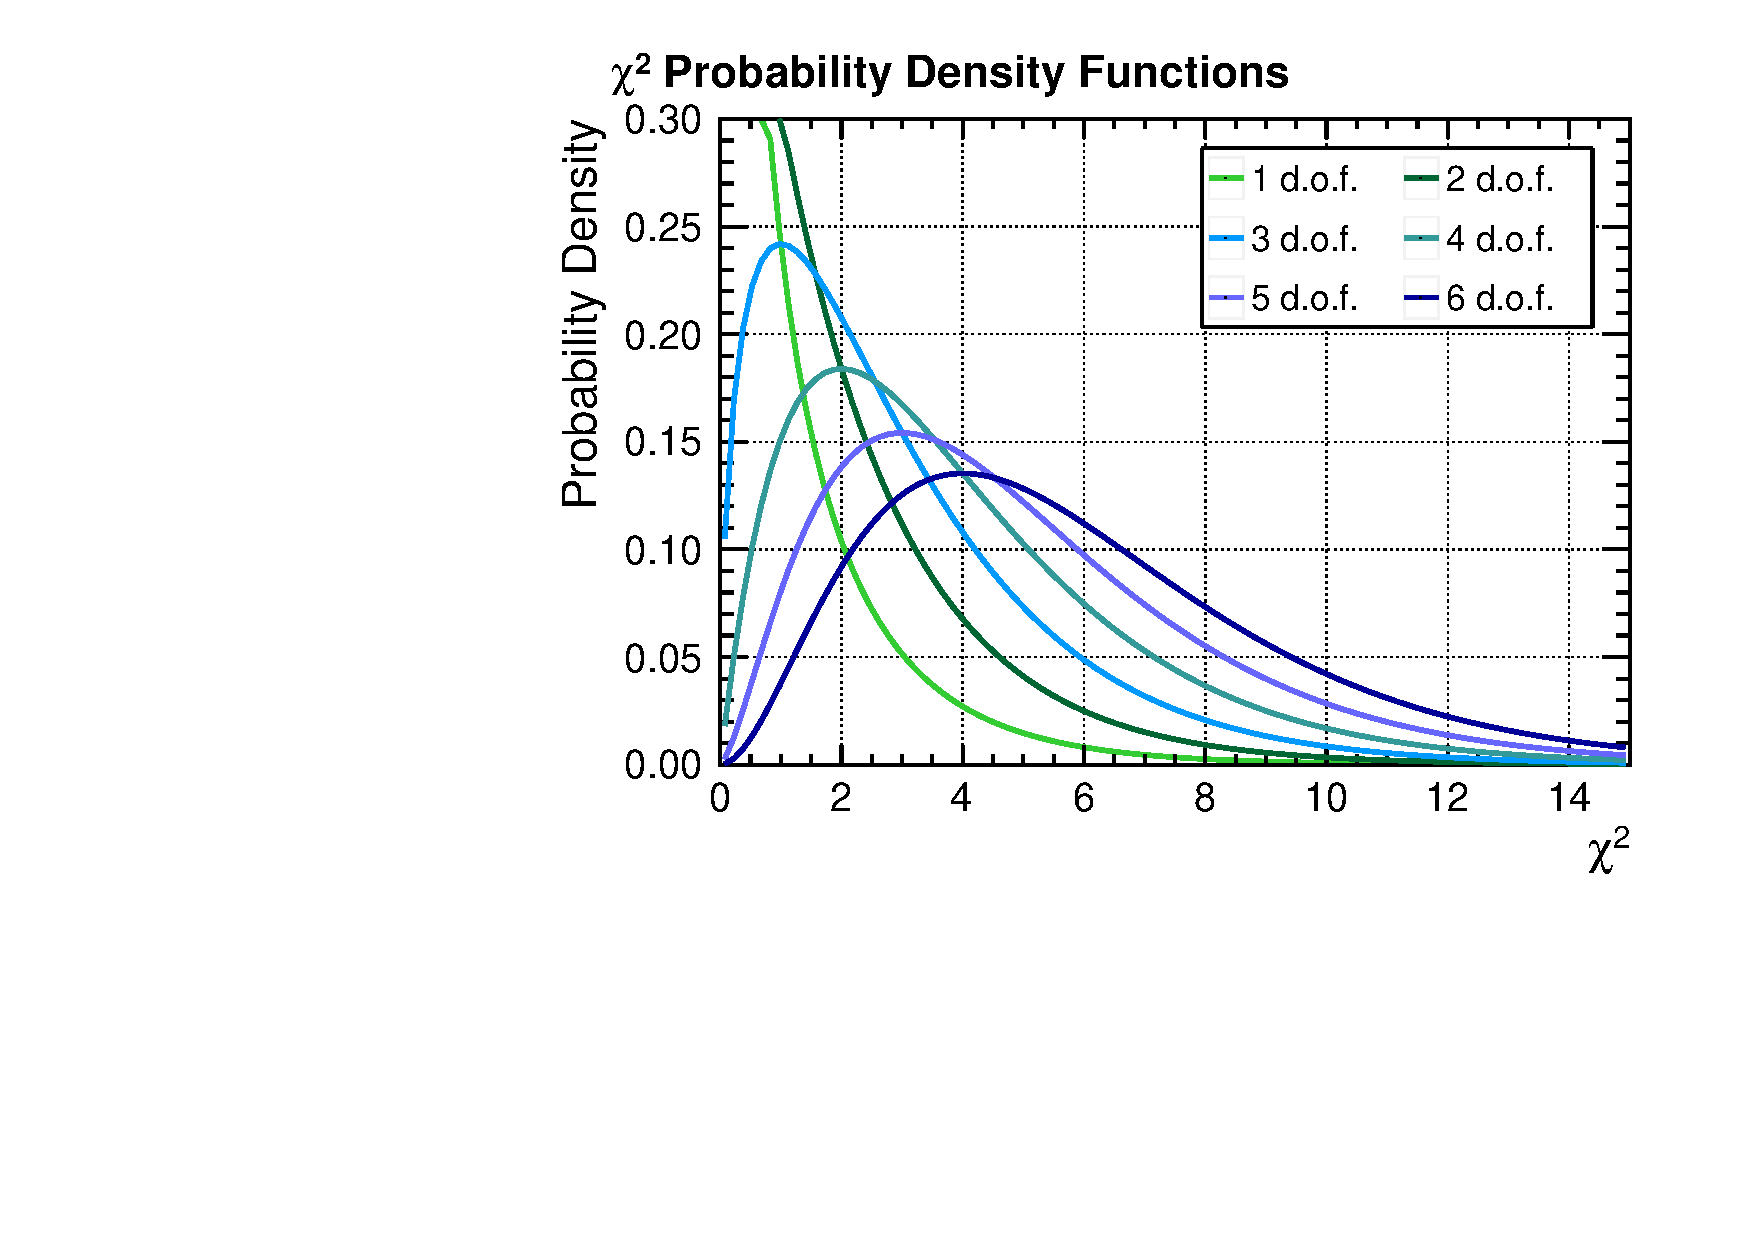
\includegraphics[width=1\textwidth]{images/chi2_normal_pdf_examples.pdf}
\caption{}
\label{fig:chi2_normal_pdf_examples.pdf}
\end{subfigure}
~ % attention ! space sensitive
\begin{subfigure}[b]{0.49\textwidth}
\centering
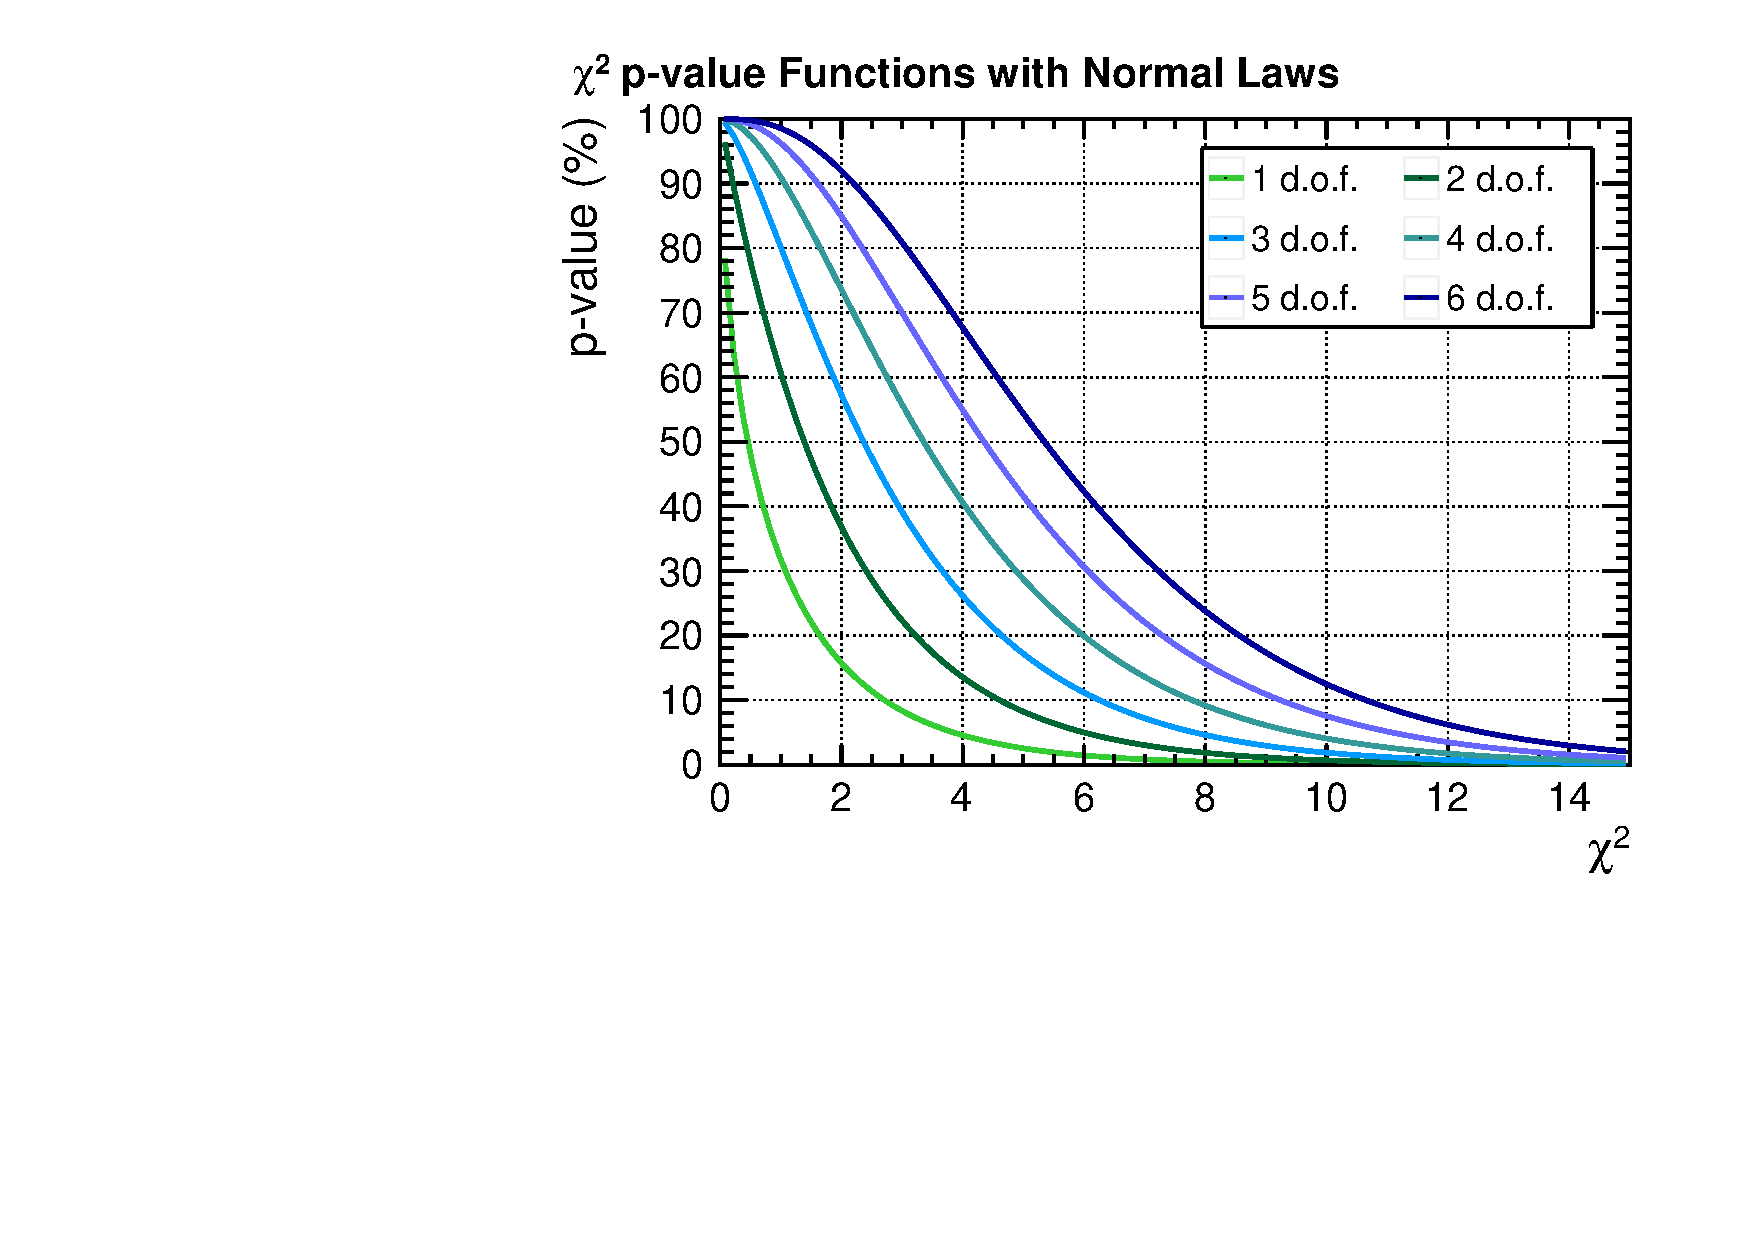
\includegraphics[width=1\textwidth]{images/chi2_p_value_functions_examples.pdf}
\caption{}
\label{fig:chi2_p_value_functions_examples.pdf}
\end{subfigure}
\caption[Exemples de lois normales de $\chi^2$]{Exemples de lois normales de $\chi^2$. (a) représente les densités de probabilité du $\chi^2$ et (b) montre la \textit{p-value} associée à chaque valeur de $\chi^2$. Les exemples sont présentés avec des nombres de degrés de liberté (d.o.f. pour \textit{degree of freedom}) allant de 1 à 6.}
\label{fig:chi2_normal_laws}
\end{figure}

}

Le terme en $\textrm{ln}\left(2\pi \left| V_\textrm{cov} \right| \right)$ ne fait pas intervenir les données, il est donc constant. L'évaluation du niveau de confiance peut alors être établie uniquement avec le $\chi^2$. En considérant que $D_i$ est une réalisation de $M_i$, la densité de probabilité du $\chi^2$ à $N$ degrés de liberté peut être écrite de la sorte:

\begin{equation}
    F(\chi^2; N) = \frac{\left( \chi^2 \right)^{N/2 -1} e^{-\chi^2/2}}{2^{N/2} \Gamma\left(\frac{N}{2}\right)},
\end{equation}

\bigbreak

où $\Gamma$ est l'extension de l'opérateur factoriel aux nombres réels: $\Gamma(n) = (n-1)!$. Dans le cadre de l'analyse d'oscillations, le nombre de degrés de liberté est le produit du nombre de bins en énergie reconstruite des spectres neutrino (11) par le nombre de cellules (6): $N = 66$. Si des paramètres libres sont ajoutés dans l'expression du $\chi^2$, il faut retirer leur nombre à $N$. Cette remarque est exploitée lors de l'analyse d'oscillation relative. De plus, il est important de remarquer que les paramètres de nuisance ne sont pas considérés comme des degrés de liberté, car leur valeur est contrainte par les \textit{pull terms}.\\

La \textit{p-value} associée à une valeur de $\chi^2_0$, obtenu avec un jeu de données $D_i$, est définie comme la fraction de pseudo-expériences générées selon le modèle $M_i$ qui ont un $\chi^2$ supérieur :

\begin{equation}
    \textit{p-value}\left(\chi^2_0,N\right) \doteq \int_{\chi^2_0}^{+\infty} d\chi^2 F(\chi^2; N).
\end{equation}

\bigbreak

La figure \ref{fig:chi2_normal_laws} montre des exemples de distributions de $F(\chi^2; N)$ et $\textit{p-value}(\chi^2_0; N)$ pour des degrés de liberté $N$ allant de 1 à 6. Alternativement, il est commun de trouver dans la littérature : le degré de réjection d'une hypothèse. Ce dernier est défini comme le complément de la \textit{p-value}, c'est-à-dire :

\begin{equation}
    \textit{exclusion C.L.}\left(\chi^2_0,N\right) = 1 - \textit{p-value}\left(\chi^2_0,N\right) = \int_{0}^{\chi^2_0} d\chi^2 F(\chi^2; N).
\end{equation}

\bigbreak

En pratique le test de $\chi^2$ est appliqué pour vérifier la validité de l'hypothèse de référence (désignée par $H_0$) qui est le scénario avec trois saveurs de neutrinos. Si $H_0$ n'est pas rejetée, c.-à-d. qu'il a une \textit{p-value} acceptable, alors l'analyse statistique se poursuit par les tests d'hypothèses alternatives $H_x$ et qui permettent de déterminer un contour d'exclusion pour un degré de confiance donné. La section suivante est consacrée au test statistique des hypothèses alternatives $H_x$.

\bigbreak

%\begin{itemize}
%    \item Définition modèle et paramètres
%    \item Densités de probabilités
%    \item Définition de la vraisemblance
%    \item Maximisation de la vraisemblance
%    \item Log L -> L gaussian distribution (taylor expansion) -> deviation in unit of sigma
%    \item Introduction chi2
%    \item En pratique H0
%\end{itemize}

\section{Tests d'hypothèses alternatives}

L'analyse statistique de motifs d'oscillation sur les spectres neutrino vise à délibérer entre plusieurs hypothèses $H_x$ dont chacune représente un scénario à 4 neutrinos désigné par  un jeu de paramètres d'oscillation $\Delta m^2$, $\textrm{sin}^2(2\theta)$. Les tests d'hypothèses alternatives permettent de dire si un scénario d'oscillation $\Delta m^2$ et $\textrm{sin}^2(2\theta)$ peut être exclu selon un niveau de confiance $\mathcal{C}$ d'après l'information apportée par la mesure $\overrightarrow{D}_0$. Le résultat de cette analyse aboutit sur la génération de \og contours d'exclusion \fg{} qui délimitent des régions de l'espace des paramètres $\Delta m^2$ et $\textrm{sin}^2(2\theta)$ rejetées par l'expérience.\\

\subsection{Interprétation des niveaux de confiance}

Nous avons vu dans la section précédente que l'inférence statistique fréquentiste se base sur le calcul de la vraisemblance qui quantifie la probabilité d'une mesure $\overrightarrow{D}_0$ sachant un modèle $\overrightarrow{M}(H_x)$. En d'autres mots, la fonction de vraisemblance est capable de fournir un intervalle $[d_1, d_2]$ qui représente une fraction $\mathcal{C}$ de la répartition des mesures D générées à partir du modèle $\overrightarrow{M}(H_x)$:

\begin{equation}
    P\left(D \in [d_1, d_2]\ |\ \mu (H_x)\right) = \mathcal{C},
\end{equation}

\bigbreak

où $\mu (H_x)$ est un paramètre du modèle $\overrightarrow{M}(H_x)$. Dans cette étude, $\mu (H_x)$ est par exemple l'amplitude des oscillations: $\textrm{sin}^2(2\theta_{14})$. Pour illustrer cette idée, des intervalles arbitraires $[d_1, d_2]$ sont dessinés sur la figure \ref{fig:statistical_inference.pdf} pour différentes hypothèses $H_x$. Ces intervalles décrivent les \og régions d'acceptation \fg{} des mesures de $D$ pour chaque $H_x$. Cependant, l'objet de cette étude est de tester la validité des hypothèses $H_x$ sachant une mesure donnée. L'inférence statistique bayésienne répond à cette problématique en introduisant un \og \textit{a priori} \fg{} qui permet d'obtenir la probabilité \og postérieure \fg{}. Cette dernière est donnée par la formule de Bayes:

\begin{equation}
    P\left(\mu | D \right) = \frac{\mathcal{L} \left(D | \mu\right) P\left(\mu \right)}{P\left(D\right)},
\end{equation}

\afterpage{
% neutron_delta_t_AmBe.pdf

\begin{figure}[h!]
\centering
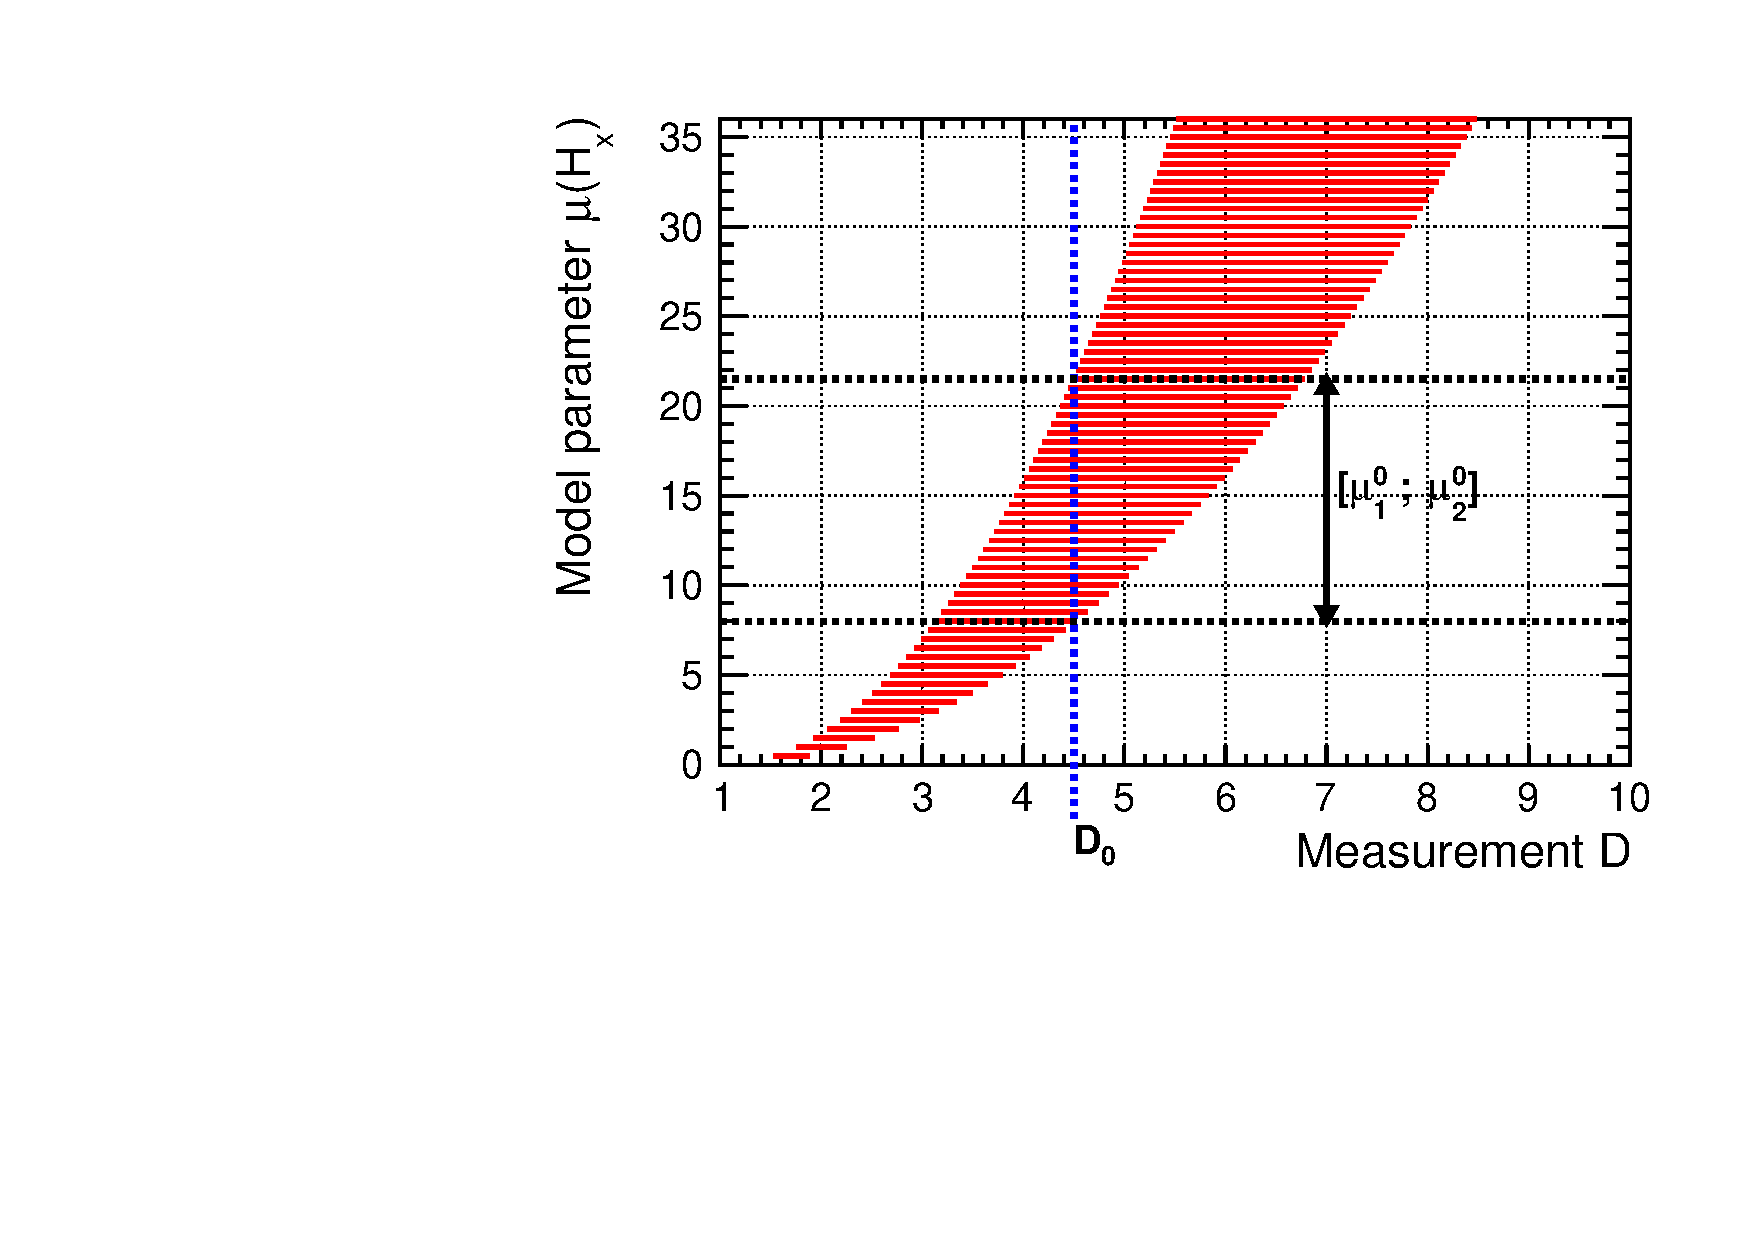
\includegraphics[width=0.75\textwidth]{images/statistical_inference.pdf}
\caption[Illustration de la détermination d'un intervalle de confiance fréquentiste]{Illustration de la détermination d'un intervalle de confiance fréquentiste. Pour un exemple de paramètre $\mu$ correspondant à une hypothèse $H_x$, un intervalle de confiance $[d_1, d_2]$ (en rouge) contenant une fraction $\mathcal{C}$ des mesures de $D$ est déterminé par la fonction de vraisemblance $\mathcal{L}(D | \mu)$. Lors d'une véritable mesure, la valeur obtenue $D_0$ est reportée (ligne hachurée en bleue) et l'intervalle de confiance $[\mu_1, \mu_2]$ est défini par l'ensemble des hypothèses acceptant $D_0$.}
\label{fig:statistical_inference.pdf}

\end{figure}

}

\bigbreak

où $P\left(\mu \right)$ est la probabilité du modèle \textit{a priori} aussi appelé \og degré de croyance \fg{}, et $P\left(D\right)$ le degré de croyance associé à $D$ qui peut être traité comme un facteur de normalisation. Il est alors possible de calculer un intervalle de crédibilité bayésien $[\mu_1; \mu_2]$ correspondant à un degré de confiance $\mathcal{C}$ lorsqu'une expérience a mesuré $D_0$:

\begin{equation}
    \int_{\mu_1}^{\mu_2} P\left(\mu | D_0 \right) d\mu = \mathcal{C}.
\end{equation}

\bigbreak

La borne $\mu_1$ peut être choisie suivant le cas de figure: limite supérieure, limite inférieure ou intervalle centré. Cependant, la difficulté d'application de la méthode bayésienne réside dans la détermination du degré de croyance $P(\mu )$. Le choix d'une fonction $P(\mu )$ objective, c'est-à-dire non informative, dépend de la métrique de $\mu$. Dans le cas des oscillations de neutrinos, choisir de sonder uniformément l'espace en $\Delta m^2_{14} \in [0; \infty]$ sur une échelle linéaire ou logarithmique ne va pas aboutir sur la même fonction postérieure $P\left(\mu | D_0 \right)$. En fait, la méthode bayésienne n'est pas adaptée pour considérer des \textit{a priori} non informatifs, car sa force réside justement  dans le fait de prendre en compte des aspects subjectifs. Par exemple son formalisme permet d'inclure les résultats des expériences précédentes, ou les croyances personnelles d'un physicien: si $\mu$ entre en contradiction avec une théorie à la fois bien fondée et \textit{vérifiée}\footnote{Une théorie n'est jamais \og vérifiée \fg{} à proprement parler. Une théorie est soit invalidée par l'expérience, soit pas encore... L'expression utilisée ici a pour but de désigner un cadre théorique qui permet d'expliquer et prédire un grand nombre de phénomènes observés sans être déjà entré en contradiction avec une mesure.} par de multiples expériences, une faible valeur $P(\mu )$ est injectée.\\

À l'inverse, la déduction statistique fréquentiste se cantonne à la fonction de vraisemblance $\mathcal{L} \left(D | \mu\right)$ sans tenter de construire une PDF selon $\mu$. En fait, un intervalle de confiance classique $[\mu_1;\mu_2]$ est membre d'un ensemble d'intervalles $\left\{ [\mu_1^i;\mu_2^i] \right\}$ (d'autres expériences) qui vérifie:

\begin{equation}
\label{eq:frequentist_interpretation}
    P(\mu^* \in [\mu_1;\mu_2]) = \mathcal{C} ,
\end{equation}

\bigbreak

où $\mu^*$ est une valeur fixée, et $\mu_1$, $\mu_2$ sont déterminés par une mesure $D$. Cette équation dit que la valeur $\mu^*$ est inclue dans une fraction $\mathcal{C}$ de tous les intervalles mesurés : $\left\{ [\mu_1^i;\mu_2^i] \right\}$. Il faut distinguer cette interprétation avec celle de la méthode bayésienne, qui affirme que le degré de croyance que la vraie valeur $\mu_\textrm{t}$ soit incluse dans l'intervalle $[\mu_1;\mu_2]$ est $\mathcal{C}$. Dans l'approche fréquentiste, l'Équation (\ref{eq:frequentist_interpretation}) est vraie pour tout $\mu^*$, alors elle est aussi vraie pour $\mu_\textrm{t}$. En pratique, $\mu_1$ et $\mu_2$ sont déterminés en testant si la valeur mesurée $D_0$ est bien dans l'intervalle $[d_1, d_2]$ dicté par chaque valeur de $\mu$. Visuellement cela se résume à tracer une ligne verticale sur $D_0$ et reporter les valeurs interceptées par les lignes rouges de la figure \ref{fig:statistical_inference.pdf}. Finalement, les contours d'oscillation représentent $\mu_1$ et $\mu_2$ pour les paramètres $\mu = \textrm{sin}^2(2\theta_{14})$ ou bien $\mu = \Delta m_{14}^2$. L'extraction des contours dans \textsc{Stereo} est effectuée en construisant une grille où chaque point représente un couple de paramètres $\textrm{sin}^2(2\theta_{14})$ et $\Delta m_{14}^2$. À chaque point est attribuée la valeur de la vraisemblance $\mathcal{L}(\overrightarrow{D} | [\textrm{sin}^2(2\theta_{14}); \Delta m_{14}^2] )$ et le contour est dessiné à l'endroit où le degré de confiance $\mathcal{C}$ est atteint.

\bigbreak

\subsection{Rapport de vraisemblance et $\Delta \chi^2$}

La question qui se pose maintenant est : quel test d'hypothèse utiliser pour maximiser la sensibilité de l'expérience ? Pour faire ce choix, nous devons distinguer deux types d'erreurs: première et seconde espèce. L'erreur de première espèce désigne le fait de rejeter une hypothèse $H_x$ à tort: soit $H_x$ définit par le couple $\Delta m^2_{14}$ et $\textrm{sin}^2(2\theta_{14})$ rejeté avec un degré de confiance $\mathcal{C}$, la probabilité de rejeter cette hypothèse à tort est $(1 - \mathcal{C})$. L'erreur de seconde espèce correspond au cas ou une hypothèse $H_x$ n'est pas rejetée alors qu'elle le devrait. Plus cette erreur est minimisée, plus le test d'hypothèse est dit \og puissant \fg{}. D'après le lemme de Neyman et Pearson \cite{1933RSPTA.231..289N}, le test d'hypothèse le plus puissant est le rapport de vraisemblances:

\begin{equation}
    R(\overrightarrow{D} ) \doteq \frac{\mathcal{L}(\overrightarrow{D} | H_x)}{\mathcal{L}(\overrightarrow{D} | H_0)},
\end{equation}


\bigbreak

où $H_0$ est l'hypothèse de référence et $H_x$ l'hypothèse en question à tester. La prescription de Feldman et Cousins \cite{Feldman:1998wt} suggère de prendre l'hypothèse de référence où la vraisemblance $\mathcal{L}(\overrightarrow{D} | H_0)$ est maximum dans l'espace des $H_x$: $H_0 \doteq H_\textrm{best fit}$. En termes de $\chi^2$, cela revient à évaluer la différence:

\begin{equation}
    \Delta \chi^2 = -2\textrm{ln}\left(R(\overrightarrow{D})\right) = \chi^2(H_x) - \chi^2(H_\textrm{best fit}) + \textrm{ln}\left( \frac{\left| V_\textrm{cov}(H_x) \right|}{\left| V_\textrm{cov}(H_\textrm{best fit} ) \right|} \right).
\end{equation}

\bigbreak

Remarquons que nous avons pris soin de garder le rapport des volumes des matrices de covariance (c'est-à-dire leur déterminant). En effet, certaines hypothèses d'oscillation peuvent faire diminuer le taux de neutrinos attendus et donc la valeur des incertitudes diminue aussi: le volume des matrices de covariance change suivant les paramètres d'oscillation. En pratique ce terme correctif n'est pas considéré dans \textsc{Stereo}. Bien que certaines hypothèses diminuent drastiquement la statistique dans quelques bins en énergie, il s'agit d'un effet local et l'impact sur les contours est négligeable.\\

%\begin{itemize}
%    \item Comparaison exclusion contours avec $\chi^2$ ou $\Delta \chi^2$
%    \item Explication : principe d'ordering
%\end{itemize}

\bigbreak

\section{Construction des contours d'exclusion}
\label{sec:building_exclision_contours}


\subsection{Méthodes conventionnelles}

En inférence fréquentiste, les méthodes conventionnelles se servent du test d'hypothèses en $\Delta \chi^2$ pour générer des contours. Elles estiment que les $\Delta \chi^2$ suivent des lois normales avec un nombre de degrés de liberté égal à celui de l'espace de $H_x$. En physique des oscillations, le $\Delta \chi^2$ a deux degrés de liberté (en $\Delta m^2_{14}$ et $\textrm{sin}^2(2\theta_{14})$) mais l'utilisation de lois normales n'est pas adaptée. C'est pour cette raison qu'en principe deux méthodes différentes sont utilisées pour établir l'inférence statistique.\\

\afterpage{

\begin{figure}[h!]
\centering
\begin{subfigure}[b]{0.49\textwidth}

\centering
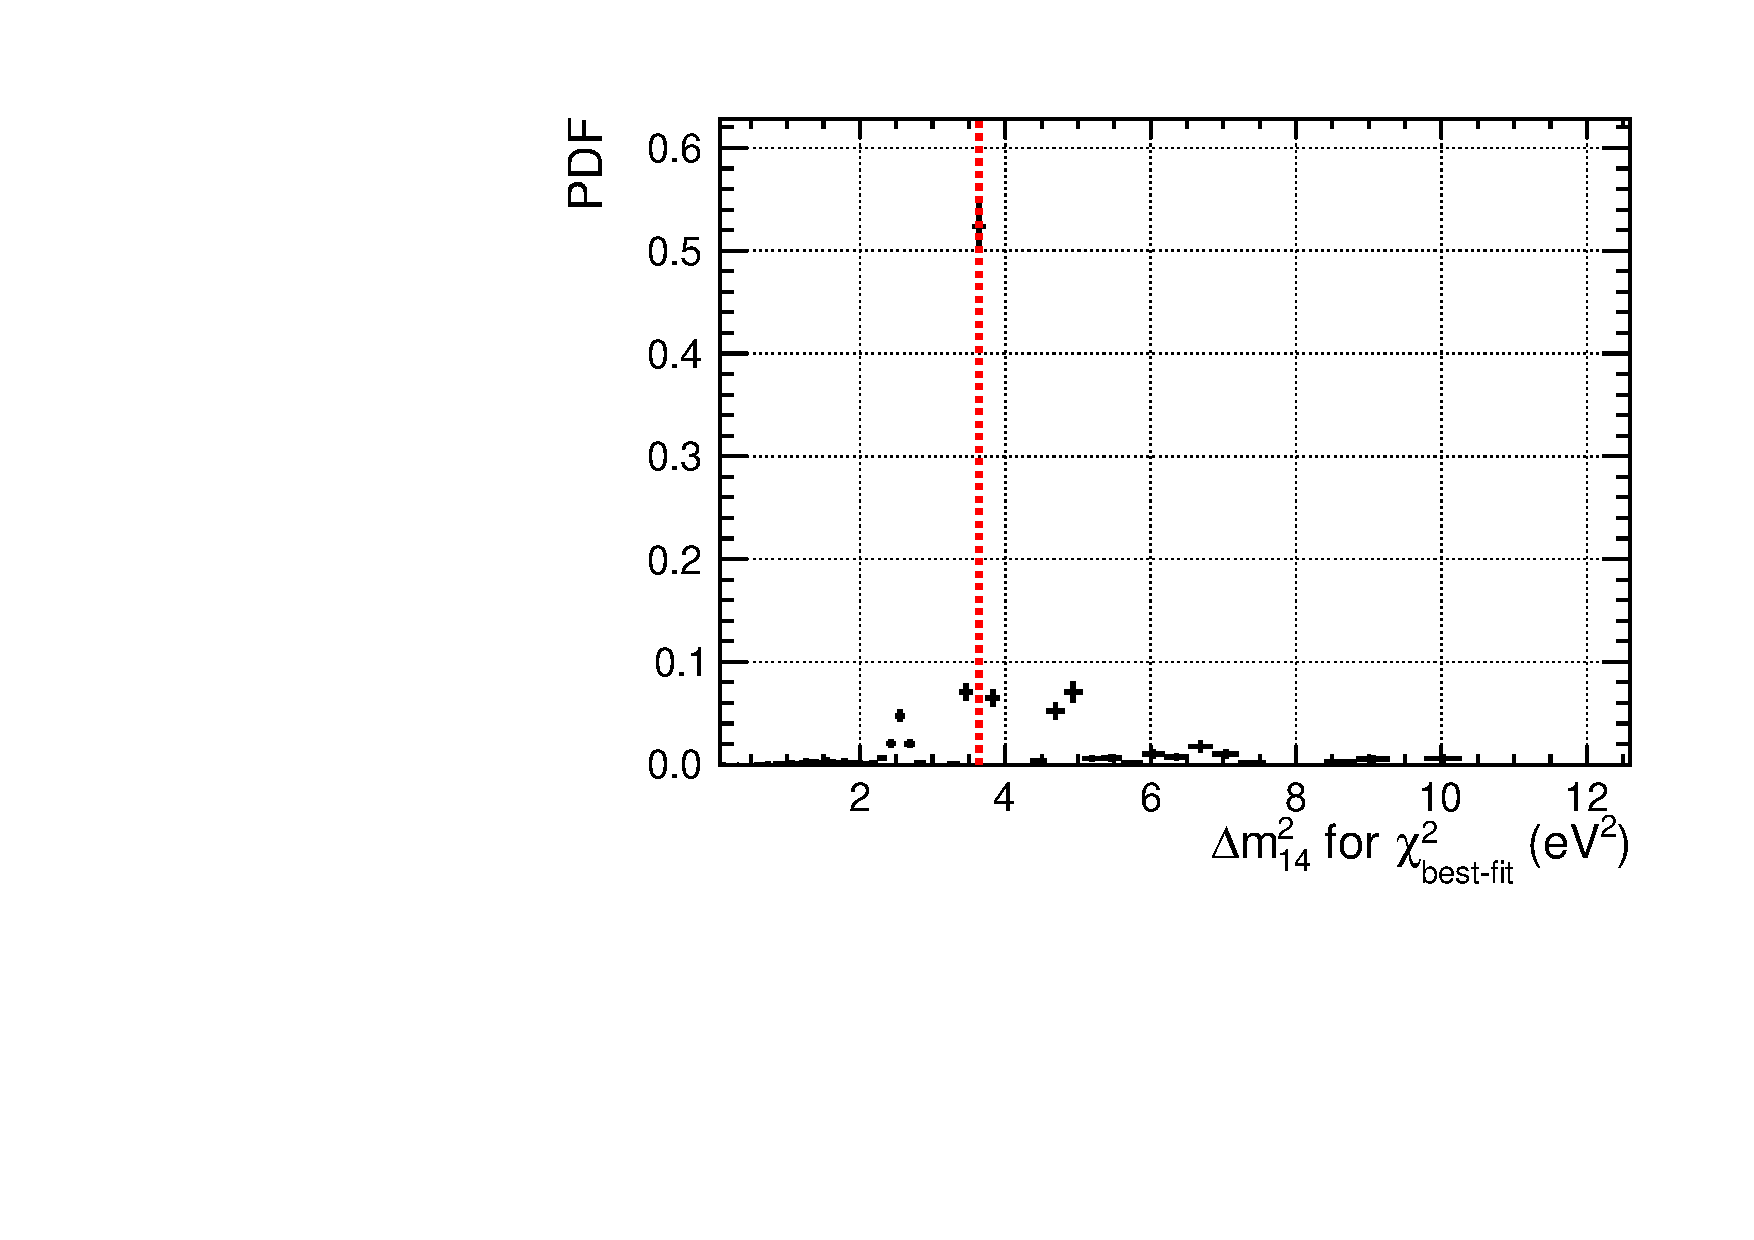
\includegraphics[width=1\linewidth]{images/profile_dm2_phase_2_3_639150_PDF_dm2-bin-75_sin2theta-bin-50.pdf}
\caption{}
\label{fig:profile_dm2_phase_2_3.828247_PDF_dm2-bin-76_sin2theta-bin-19.pdf}

\end{subfigure}
~ % attention ! space sensitive
\begin{subfigure}[b]{0.49\textwidth}

\centering
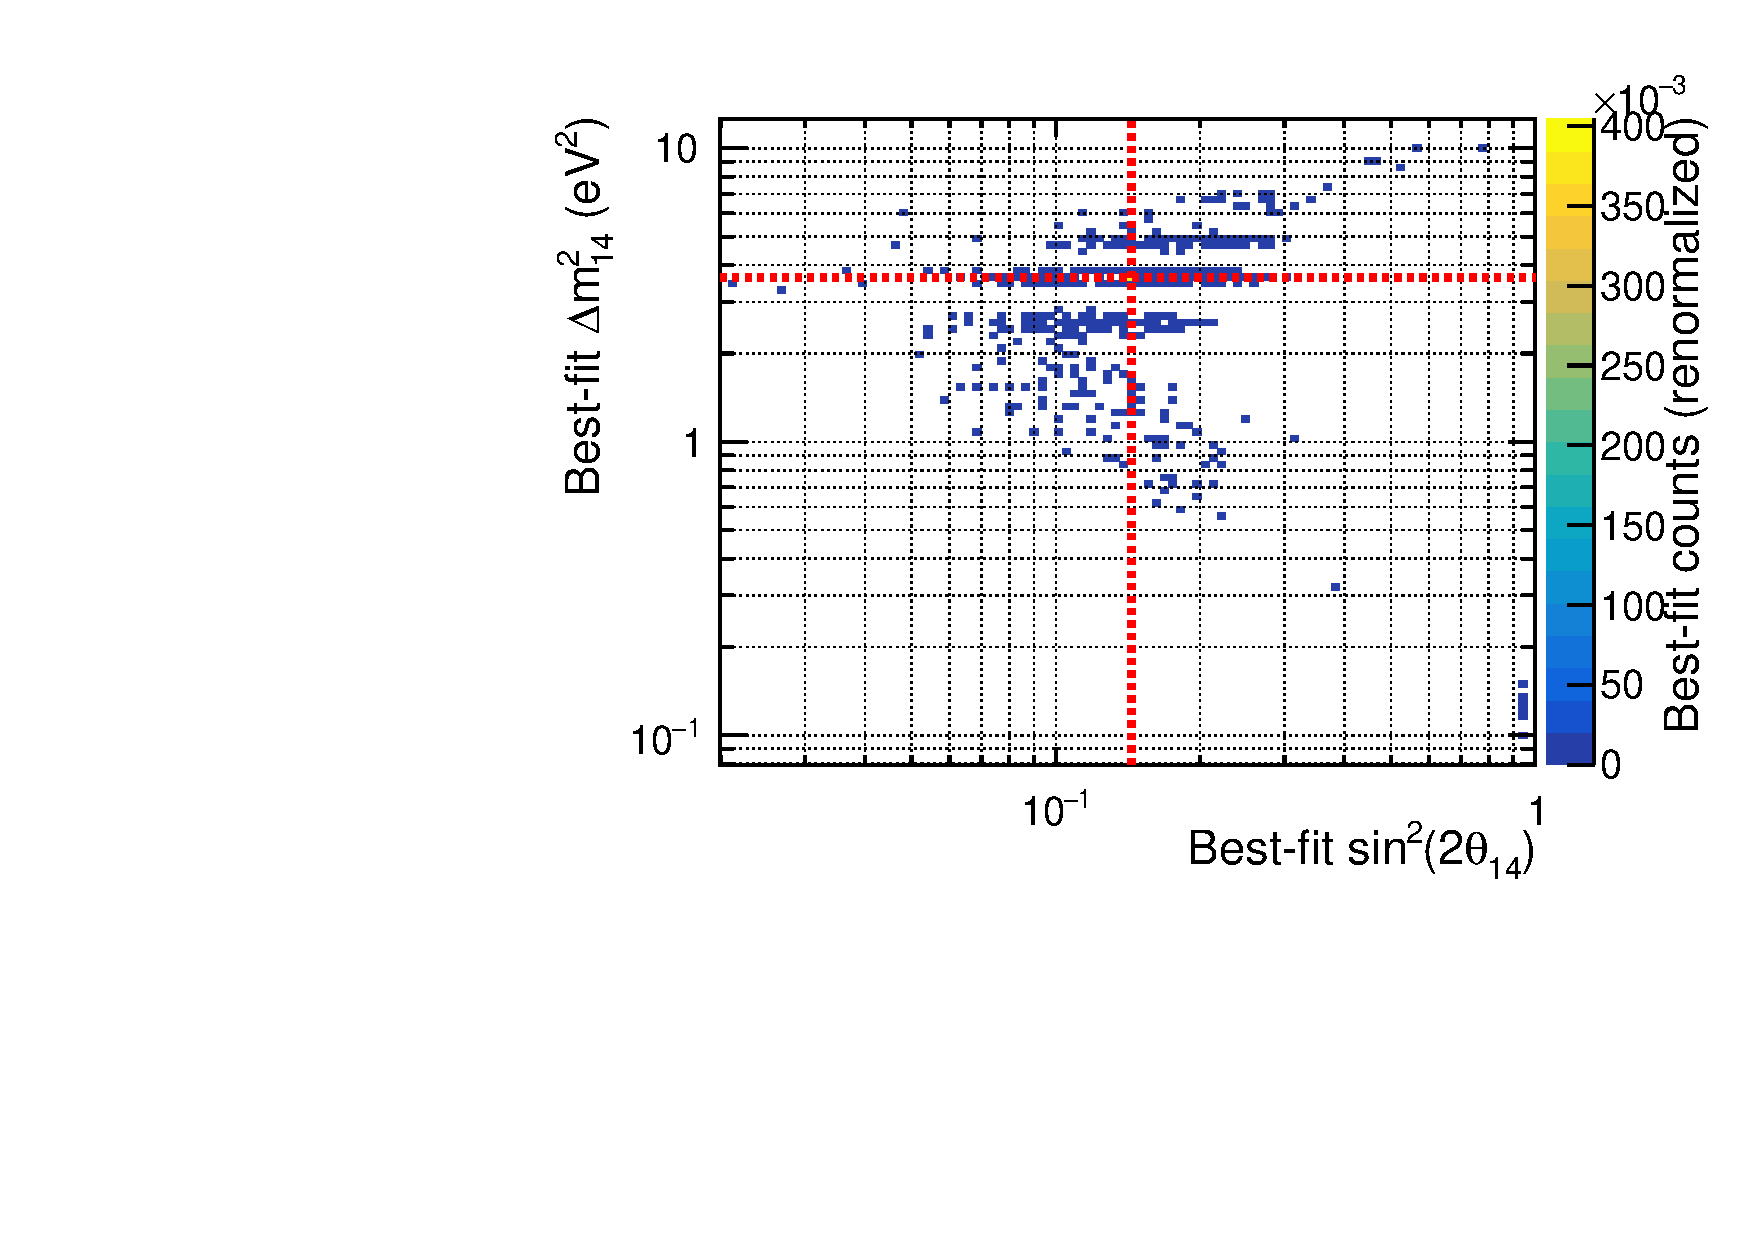
\includegraphics[width=1\linewidth]{images/best_fit_PDF_3_639150_0_144046.pdf}
\caption{}
\label{fig:best_fit_PDF_3.828247_0.042806.pdf}

\end{subfigure}
\caption[Distributions des valeurs $\Delta m^2_{14}$ au \textit{best-fit} (\textit{global-scan}) sur un jeu de données généré par simulation]{Distributions des valeurs $\Delta m^2_{14}$ au \textit{best-fit} (\textit{global-scan}) sur un jeu de données généré par simulation. L'hypothèse de départ est désignée par la ligne en pointillé rouge. La déduction en niveau de confiance par la méthode du \textit{global-scan} présume que les PDFs de $\Delta m_{14}^2$ suivent des lois gaussiennes. (a) montre que les valeurs de $\Delta m_{14}^2$ du \textit{best-fit} ne sont pas distribuées selon une gaussienne et (b) montre la répartition des \textit{best-fits} sur le plan $\Delta m_{14}^2$, $\textrm{sin}^2(2\theta_{14})$. L'hypothèse injectée est : $\Delta m_{14}^2 = \SI{3.6}{eV^2}$, $\textrm{sin}^2(2\theta_{14}) = 14\%$.}
\label{fig:profile_dm2}
\end{figure}
%%%%%%%%%%%%%%%%%%%%%%%%%%%%%%%%%%%%
%\begin{figure}[h!]
%\centering
%\begin{subfigure}[b]{0.49\textwidth}
%
%\centering
%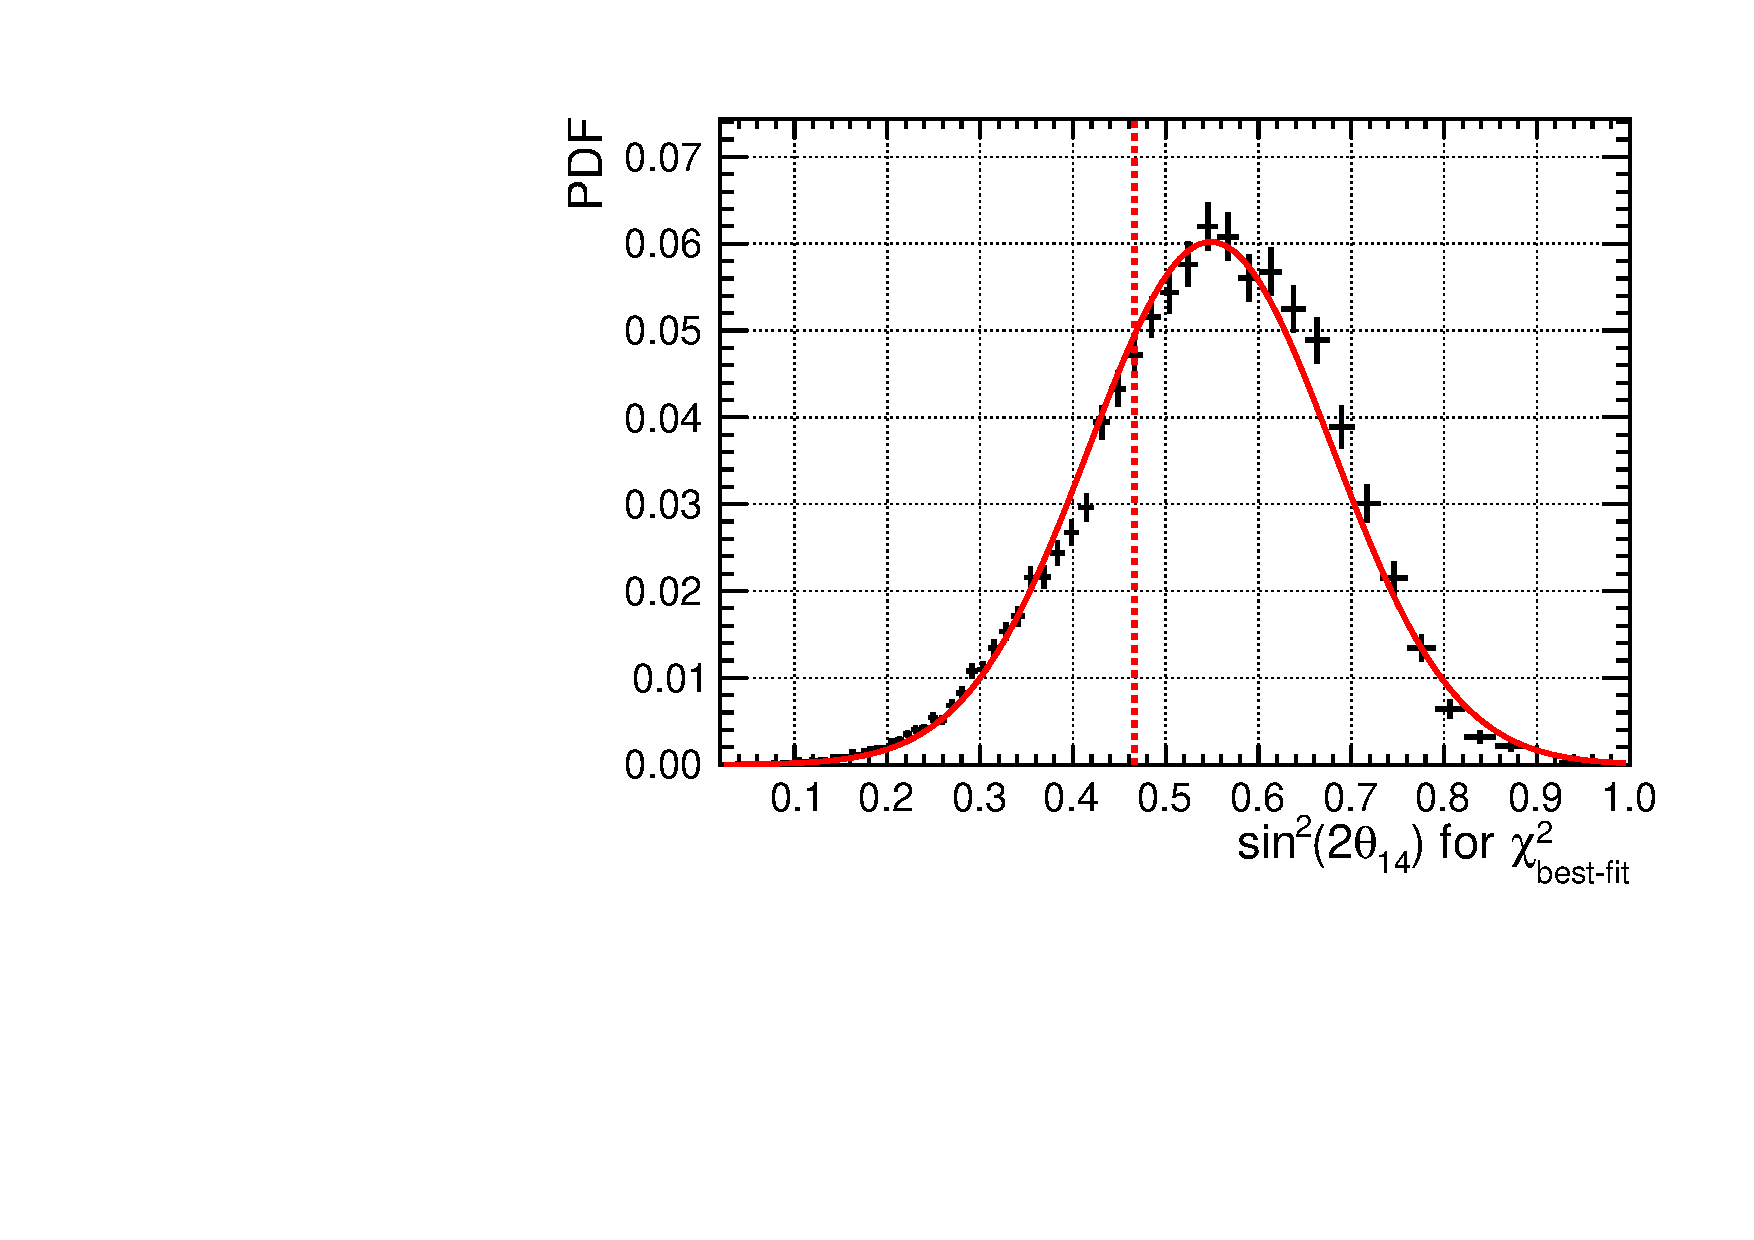
\includegraphics[width=1\linewidth]{images/profile_sin2theta_phase_1_0_466122_PDF_dm2-bin-50_sin2theta-bin-80.pdf}
%\caption{Erreurs statistiques équivalentes à la phase 1.}
%\label{fig:profile_sin2theta_phase_1_0_466122_PDF_dm2-bin-50_sin2theta-bin-80.pdf}
%
%\end{subfigure}
%~ % attention ! space sensitive
%\begin{subfigure}[b]{0.49\textwidth}
%
%\centering
%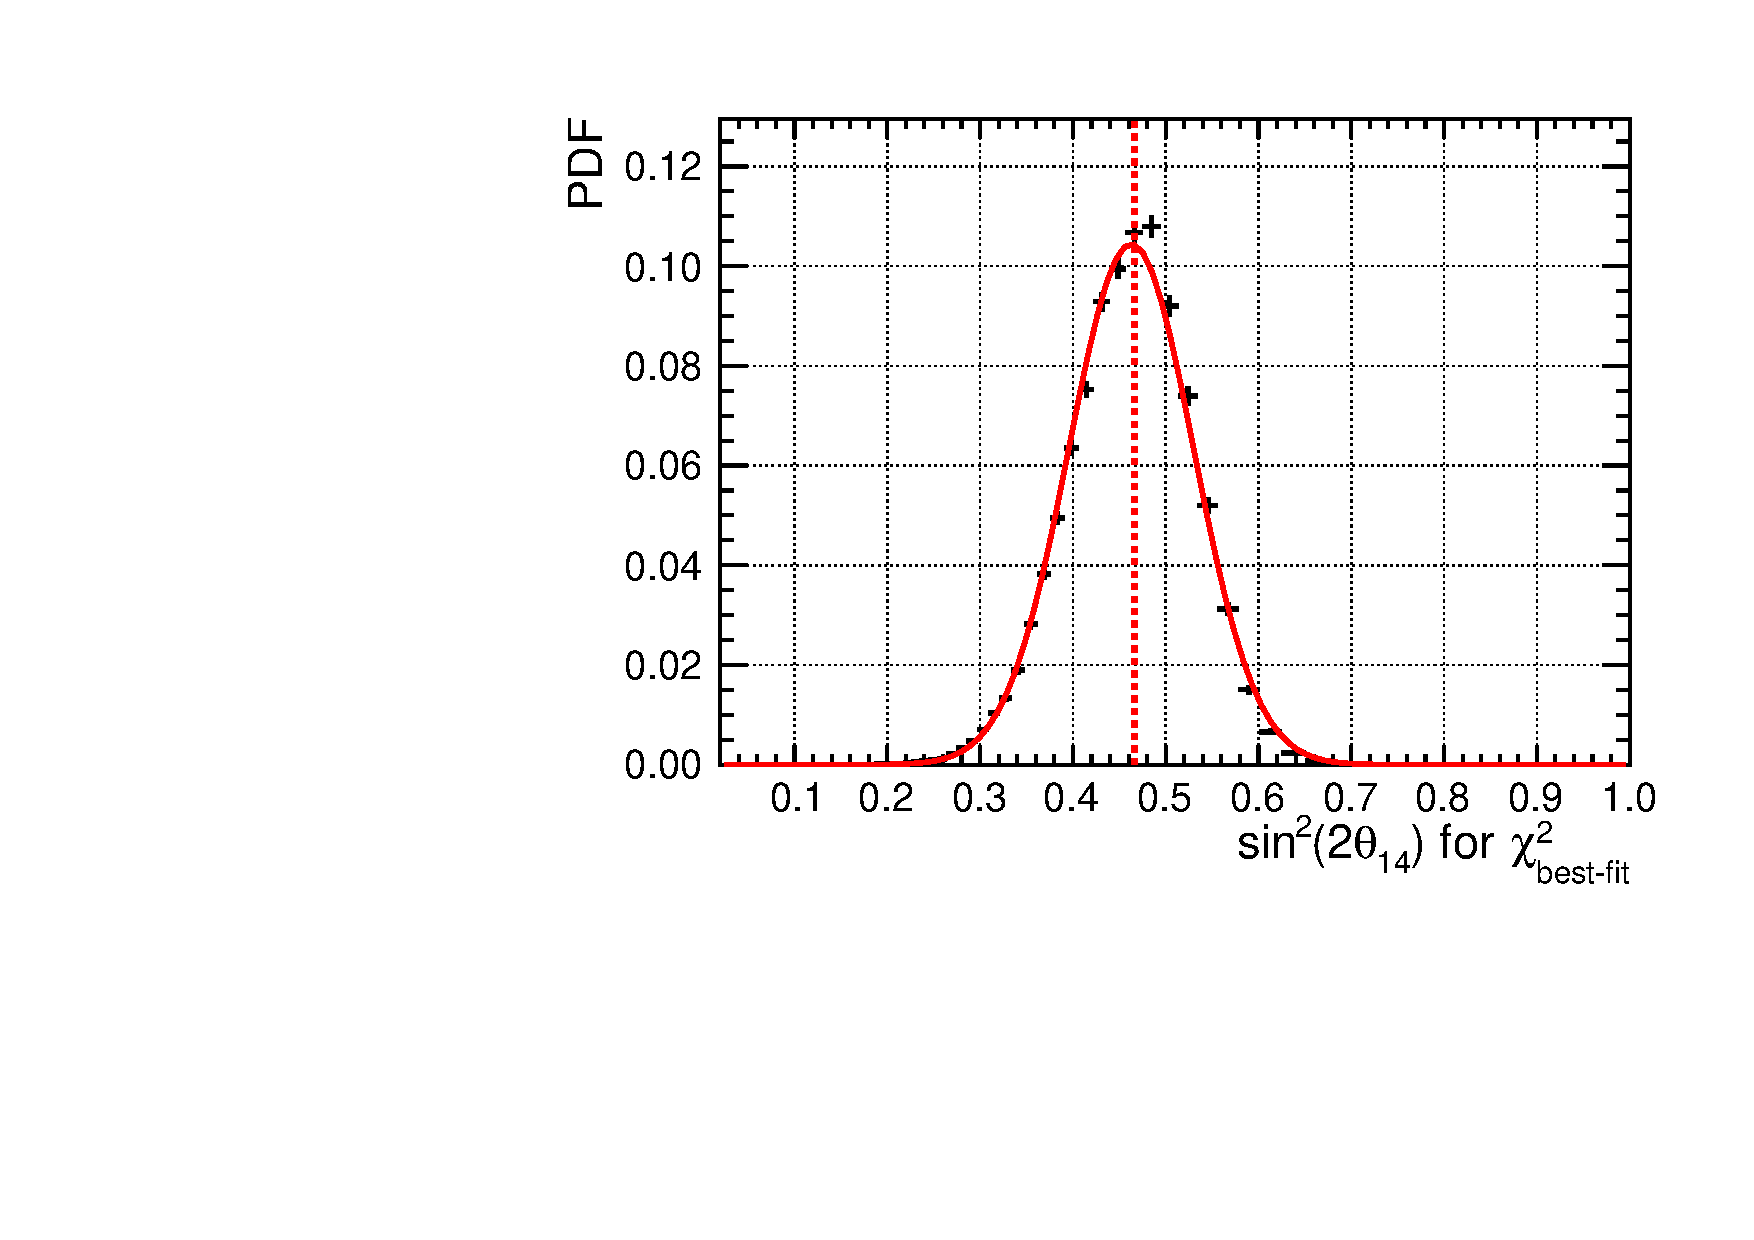
\includegraphics[width=1\linewidth]{images/profile_sin2theta_phase_2_0_466122_PDF_dm2-bin-50_sin2theta-bin-80.pdf}
%\caption{Erreurs statistiques équivalentes à la phase 2.}
%\label{fig:profile_sin2theta_phase_2_0_466122_PDF_dm2-bin-50_sin2theta-bin-80.pdf}
%
%\end{subfigure}
%\caption[Distributions des valeurs $\textrm{sin}^2(2\theta_{14}))$ qui minimisent le $\chi2$ sur un jeu de données généré par simulation]{Distributions des valeurs $\textrm{sin}^2(2\theta_{14}))$ qui minimisent le $\chi2$ sur un jeu de données généré par simulation à $\Delta m^2_{14}$ fixé. L'hypothèse de départ est désignée par la ligne rouge en pointillé. La courbe rouge est une fonction gaussienne fittée à comparer avec la véritable PDF mesurée (noir). En phase 2 (b) la distribution est une gaussienne centrée sur la valeur injectée alors qu'en phase 1 (a) cette dernière est décentrée vers les valeurs .}
%\label{fig:profile_sin2theta}
%\end{figure}

\begin{figure}[h!]

\centering
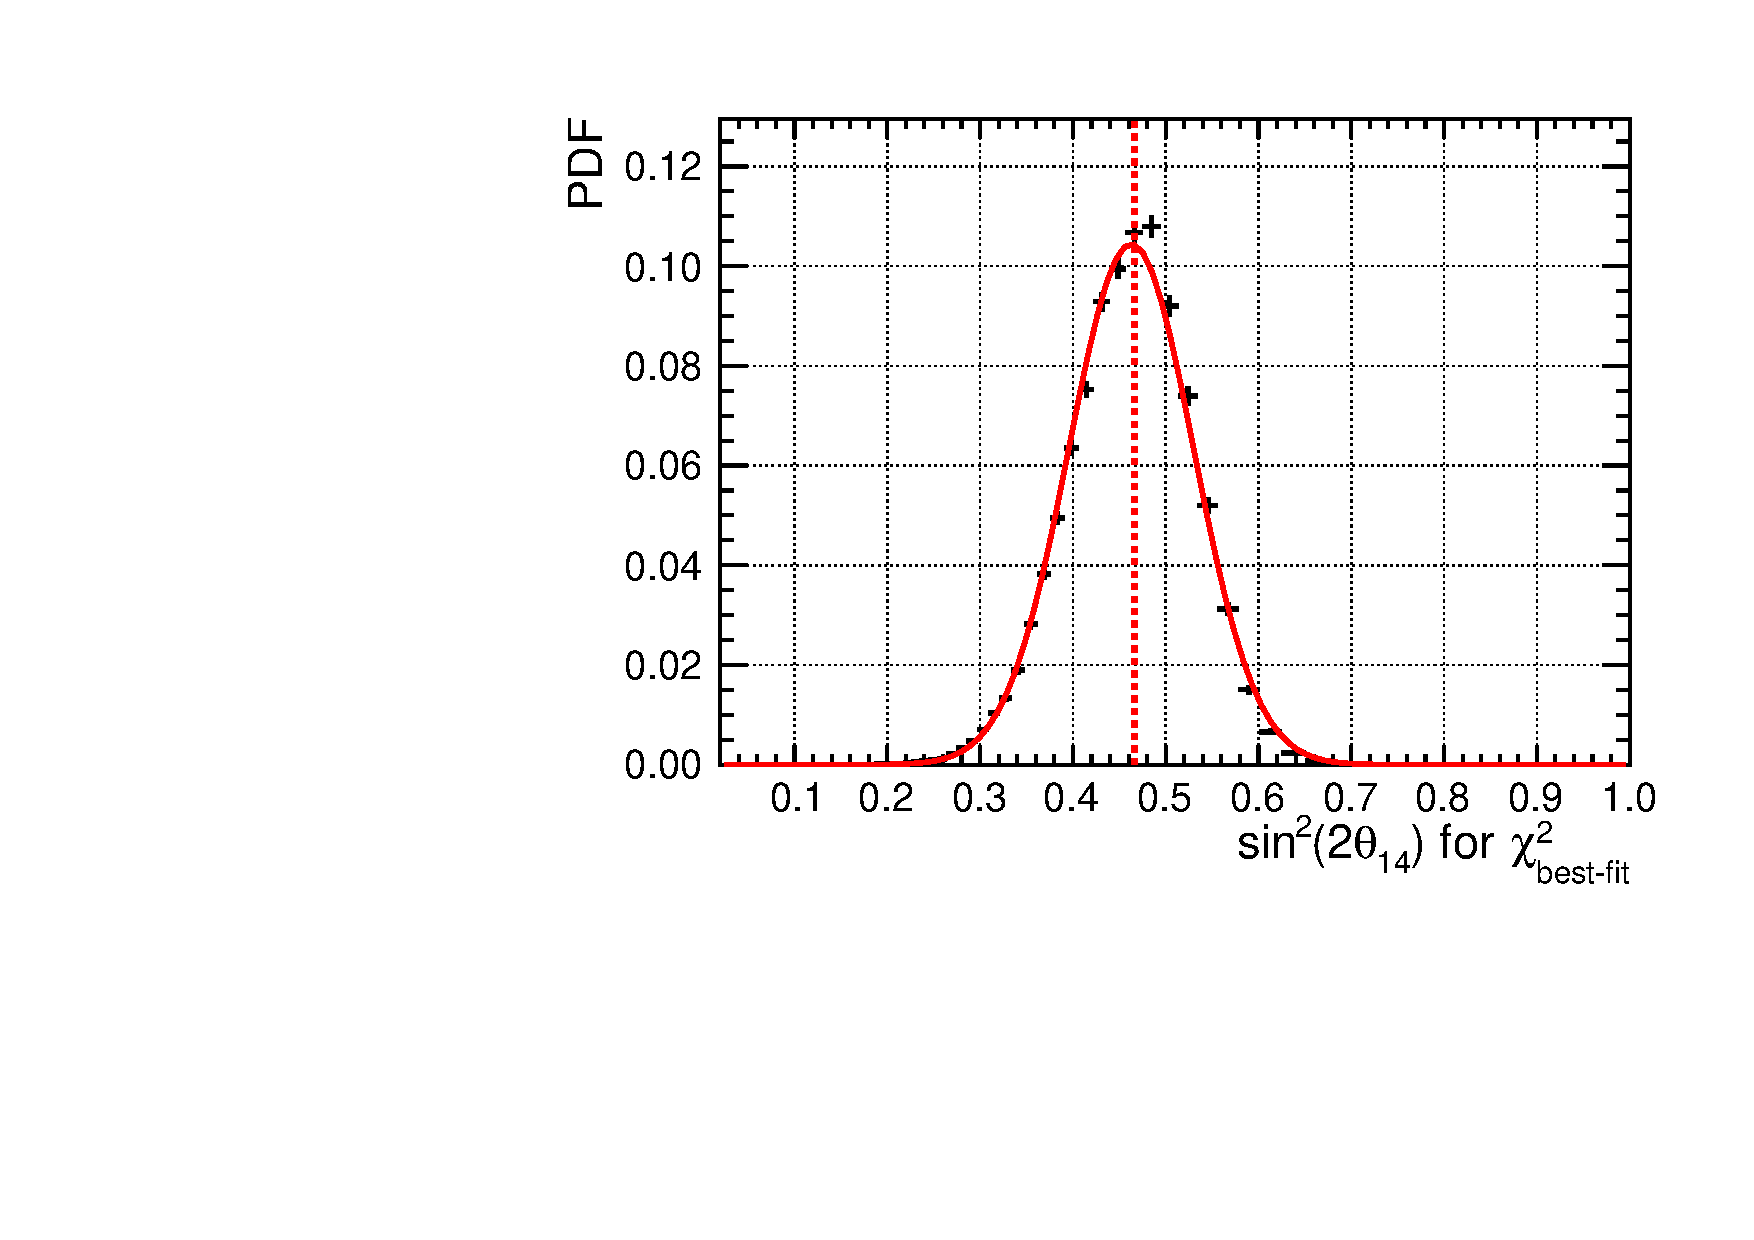
\includegraphics[width=0.6\linewidth]{images/profile_sin2theta_phase_2_0_466122_PDF_dm2-bin-50_sin2theta-bin-80.pdf}
\caption[Distributions des valeurs $\textrm{sin}^2(2\theta_{14}))$ au \textit{best-fit} (\textit{raster-scan}) sur un jeu de données généré par simulation]{Distributions des valeurs $\textrm{sin}^2(2\theta_{14}))$ au \textit{best-fit} (\textit{raster-scan}) sur un jeu de données généré par simulation. L'hypothèse de départ est désignée par la ligne rouge en pointillé. La courbe rouge est une fonction gaussienne fittée à comparer avec la véritable PDF mesurée (noir).}
\label{fig:profile_sin2theta}

\end{figure}

}

\subsubsection*{Le global-scan}

Le \og \textit{global scan} \fg{}  consiste à chercher la position du \textit{best-fit} sur une gamme définie au préalable en $\Delta m^2_{14}$ et $\textrm{sin}^2(2\theta_{14})$, et déduire le degré de confiance de chaque hypothèse par des lois normales à deux degrés de liberté selon $\Delta \chi^2 (\Delta m^2_{14}, \textrm{sin}^2(2\theta_{14}))$. Le souci de cette méthode réside dans la nature sinusoïdale des motifs d'oscillation en $\Delta m^2_{14}$. En effet, l'utilisation d'une loi normale pour déduire le degré de confiance nécessite que $M_{cb}$ soit linéaire en $\Delta m^2_{14}$. Or cette condition n'est pas satisfaite:

\begin{equation}
    \frac{\partial M_{cb}}{\partial \Delta m^2} \propto \frac{\partial \textrm{sin}^2\left(\frac{\Delta m^2 L_c}{E_b} \right)}{\partial \Delta m^2} = \frac{L_c}{E_b} \textrm{sin}\left(\frac{2\Delta m^2 L_c}{E_b}\right)
\end{equation}

\bigbreak

où $L_c$ et $E_b$ sont déterminés par la position de la cellule $c$ et le bin en énergie $b$ respectivement. Cela signifie que la densité de probabilité selon $\Delta m^2$ n'est pas une gaussienne (cf. figure \ref{fig:profile_dm2_phase_2_3.828247_PDF_dm2-bin-76_sin2theta-bin-19.pdf}), donc le $\Delta \chi^2$ ne suit pas une loi normale. En pratique, les fluctuations statistiques peuvent s'harmoniser avec des scénarios très différents en $\Delta m^2_{14}$, c'est-à-dire physiquement très éloigné de l'hypothèse de départ : voir figure \ref{fig:best_fit_PDF_3.828247_0.042806.pdf}. Cet effet augmente ainsi artificiellement la valeur de $\Delta \chi^2$. C'est pourquoi les contours obtenus avec le \textit{global scan} ont tendance à surestimer le pouvoir de discrimination d'une expérience.\\

\subsubsection*{Le raster-scan}

Le \og \textit{raster-scan} \fg{} (balayage de trame) s'affranchit de la dépendance en $\Delta m_{14}^2$ en fixant sa valeur dans le $\Delta \chi^2$. Pour un scénario d'oscillation donné $(\Delta m_{14}^2, \textrm{sin}^2(2\theta_{14}))$, le \textit{best fit} est recherché sur une tranche de valeurs $\textrm{sin}^2(2\theta_{14}))$ à $\Delta m_{14}^2$ constant. La déduction statistique est effectuée en se référent à une loi de $\chi^2$ normale à un degré de liberté. Cette méthode présuppose que la fonction de propagation $M_{cb}$ est linéaire selon $\textrm{sin}^2(2\theta_{14})$. Cette hypothèse est valide \textit{de facto} car les spectres oscillé sont générés avec (cf. Section \ref{sec:building_oscillation}):

\begin{equation}
\begin{gathered}
    M_{cb}^\textrm{osc} \left(\Delta m_{14}^2, \textrm{sin}^2(2\theta_{14})\right) = M_{cb}^\textrm{non-osc} \times \left[1 - \textrm{sin}^2(2\theta_{14}) \left( 1 - R_{cb}(\Delta m_{14}^2) \right)\right],\\
    \textrm{donc : } \frac{\partial M_{cb}^\textrm{osc}}{\partial \textrm{sin}^2(2\theta_{14})} = - M_{cb}^\textrm{non-osc} \times R_{cb}(\Delta m_{14}^2) = f\left(\Delta m^2_{14}, \cancel{\textrm{sin}^2(2\theta_{14})} \right).
\end{gathered}
\end{equation}

\bigbreak

De plus, cette hypothèse a été vérifiée en montrant à l'aide de pseudo-expériences que la répartition des $\textrm{sin}^2(2\theta)$ au \textit{best-fit} suit une loi gaussienne : voir figure \ref{fig:profile_sin2theta}. On remarquera néanmoins que les valeurs de $\textrm{sin}^2(2\theta)$ sont bornées entre 0 et 1, donc le comportement gaussien n'est valide que suffisamment loin de ces bornes. Le \og suffisamment \fg{} est défini par la largeur caractéristique des gaussiennes, qui dépend de la taille des barres d'erreurs. Finalement, l'inconvénient du \textit{raster-scan} repose sur le fait qu'en traitant chaque tranche en $\Delta m^2_{14}$ séparément, cette méthode n'est pas en mesure de désigner quelles valeurs en $\Delta m^2_{14}$ sont les plus probables. Cela peut notamment avoir comme effet de créer des zones d'exclusion partant de $\textrm{sin}^2(2\theta) = 0$, suggérant le rejet de l'hypothèse nulle $H_0$. Lors d'un signal positif (découverte d'un neutrino stérile), la zone couverte par le contour ne distingue pas les valeurs vraisemblables de $\Delta m^2$ contrairement au \textit{global-scan}.\\

Afin de tirer parti des avantages des deux méthodes, à savoir bonne estimation du pouvoir de réjection et discrimination suivant des tranches en $\Delta m^2$, Feldman et Cousins \cite{Feldman:1998wt} ont montré qu'il est nécessaire de construire des lois sur mesure en $\Delta\chi^2$ en générant des \og pseudo-expériences \fg{}. C'est la discussion qui est entreprise dans la section suivante.

\bigbreak

\subsection{Création de PDFs sur-mesure en $\Delta \chi^2$}
\label{sec:custom_PDF_generation}

\afterpage{

\begin{figure}[h!]

\centering
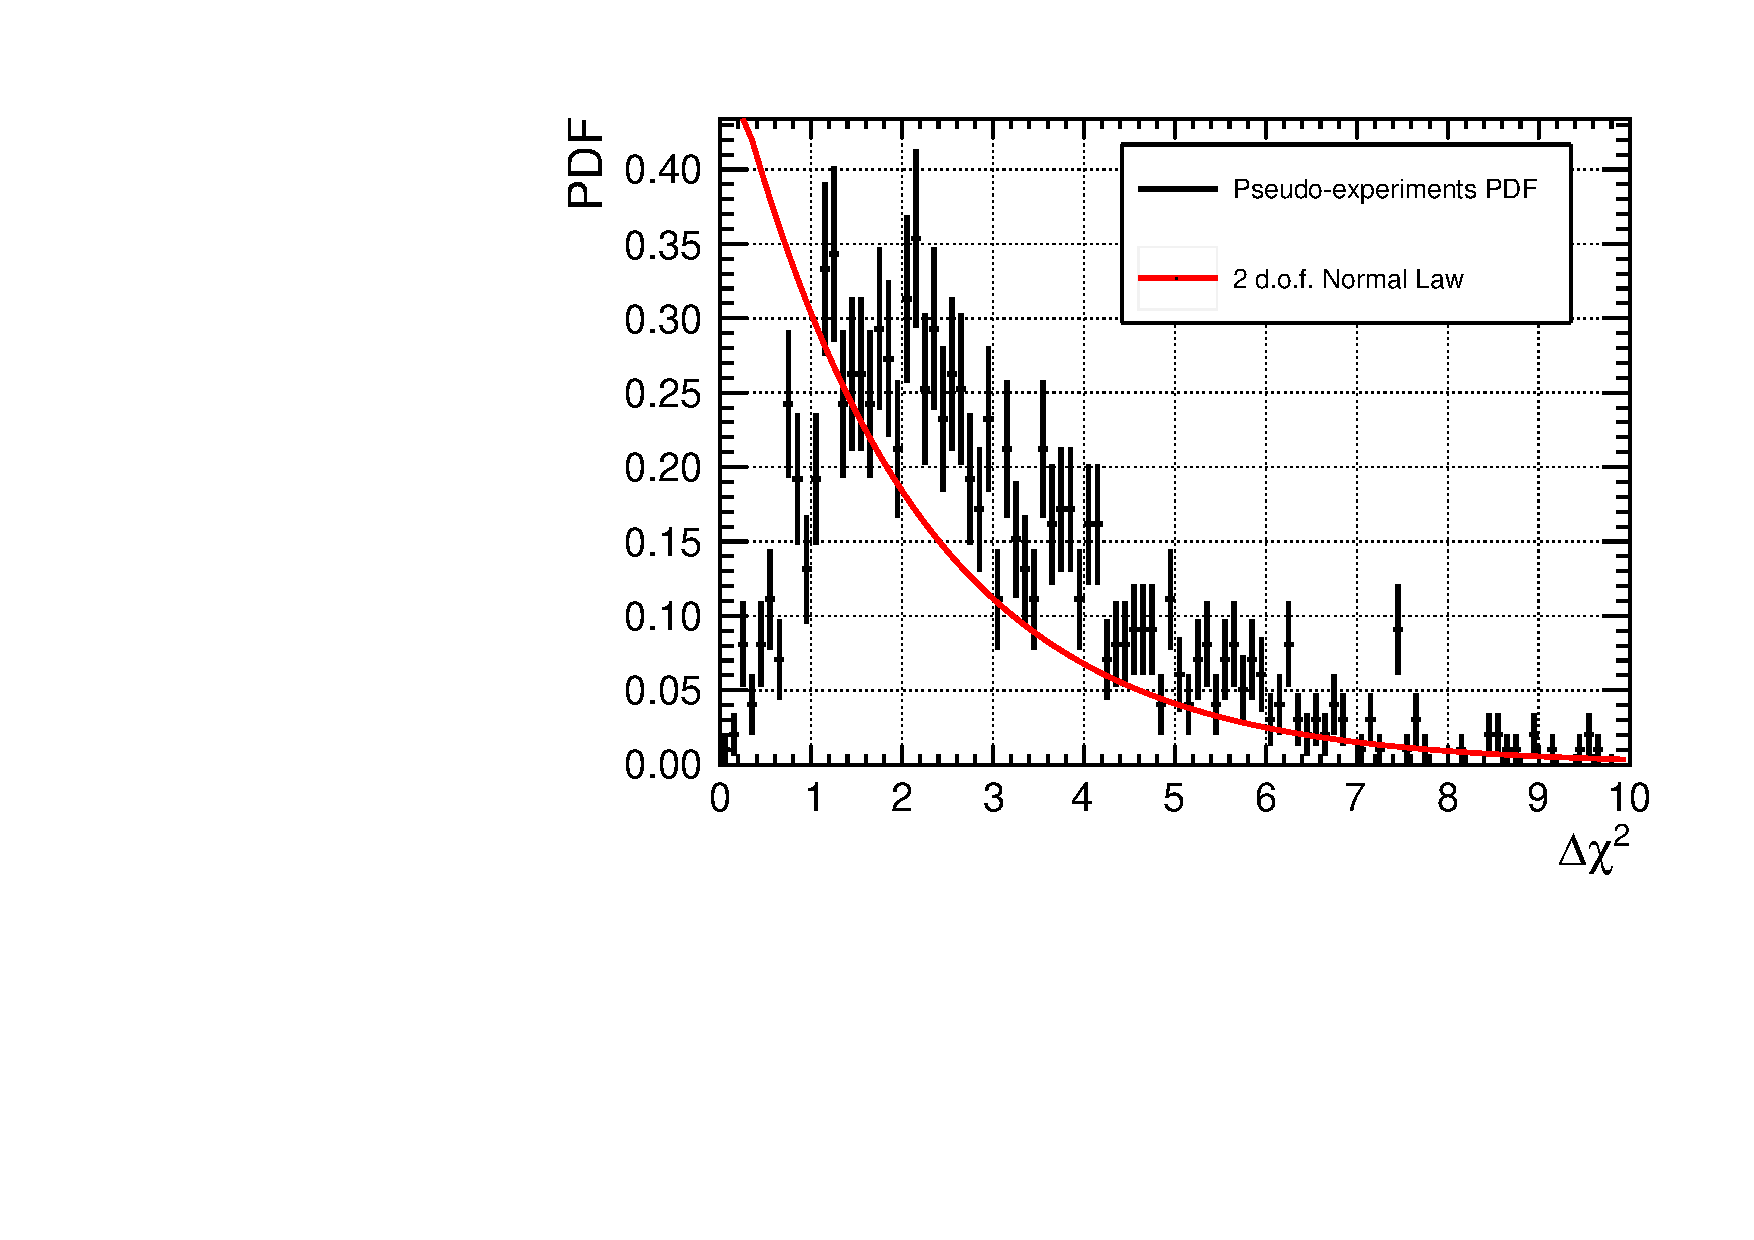
\includegraphics[width=0.7\linewidth]{images/delta_chi2_pdf_vs_normal_-1_-1.pdf}
\caption[Comparaison de la PDF de $\Delta\chi^2$ généré par pseudo-expériences avec la loi normale de $\chi^2$ à deux degrés de liberté]{Comparaison de la PDF de $\Delta\chi^2$ généré par pseudo-expériences avec la loi normale de $\chi^2$ à deux degrés de liberté.}
\label{fig:delta_chi2_pdf_vs_normal_-1_-1.pdf}

\end{figure}

}

La zone du plan $\Delta m^2_{14}, \textrm{sin}^2(2\theta_{14})$ exclue avec un degré de confiance $\mathcal{C}$ est construite en faisant un grand nombre de \og pseudo-expériences \fg{} par simulations MC. Une pseudo-expérience $M_{cb}^*$ est générée à partir des valeurs des données Asimov ($M_{cb}$) dans le cadre d'une hypothèse d'oscillation choisie sur la grille : $\left(\Delta m^2_{14}, \textrm{sin}^2(2\theta_{14})\right)$. À chaque bin $M^*_{cb}$ est attribué une distorsion tirée au hasard dans les distributions d'incertitudes statistiques et systématiques. Le spectre $M^*_{cb}$ est injecté dans le $\chi^2$ à la place des données $D_{cb}$, et ce dernier est minimisé avec les paramètres de nuisance (si présents). Avec ce même échantillon $M^*_{cb}$, le $\chi^2$ est calculé pour tous les points de la grille en $\textrm{sin}^2(2\theta)$ et $\Delta m^2$ pour la méthode \textit{global-scan}, tous les points en $\textrm{sin}^2(2\theta)$ à $\Delta m^2$ fixé pour la méthode \textit{raster-scan}, afin de déterminer le \textit{best fit}. Enfin la valeur de $\Delta\chi^2 = \chi^2 - \chi^2_\textit{best fit}$ est enregistré pour cette pseudo-expérience. La procédure est répétée un grand nombre de fois afin d'obtenir la PDF des $\Delta\chi^2$ ($F(\Delta\chi^2)$) associés à l'hypothèse considérée : $\Delta m^2_{14}, \textrm{sin}^2(2\theta_{14})$. Un exemple de PDF de $\Delta\chi^2$ est comparé avec une loi normale à deux degrés de liberté sur la figure \ref{fig:delta_chi2_pdf_vs_normal_-1_-1.pdf}. Finalement, le degré de confiance de réjection est déduit en intégrant ces distributions jusqu'au $\Delta\chi^2_0$ obtenu avec les vraies données:

\begin{equation}
    \textit{exclusion C.L.}\left(\Delta\chi^2_0 \right) = \int_{0}^{\Delta\chi^2_0} d\Delta\chi^2 F\left(\Delta\chi^2, \Delta m_{14}^2, \textrm{sin}^2(2\theta_{14})\right).
\end{equation}

\bigbreak

En pratique, les $\Delta\chi^2$ sont classés par ordre croissant et enregistrés dans un \texttt{TTree}. Le niveau de confiance est évalué en comptant le nombre de pseudo-expériences qui ont un $\Delta\chi^2$ plus faible que celui des données :

\begin{equation}
    \textit{exclusion C.L.}\left(\Delta\chi^2_0 \right) = \frac{\textrm{nb pseudo-expériences tel que } \Delta\chi^2 < \Delta\chi^2_0}{\textrm{nb pseudo-expériences}}.
\end{equation}

\bigbreak

Il est important de noter que cette procédure est extrêmement couteuse en temps de calcul. En effet, pour chaque pseudo-expérience, il est nécessaire de trouver le \textit{best fit} sur toute la grille en $\Delta m^2_{14}, \textrm{sin}^2(2\theta_{14})$. À cause de la non linéarité de $M_{cb}$ par rapport à $\Delta m^2_{14}$,  l'utilisation d'algorithmes de minimisation par gradient comme \texttt{TMinuit} n'est pas envisageable. En définitive la minimisation est effectuée en trouvant le $\chi^2$ minimum dans chaque tranche en $\Delta m^2_{14}$, et la valeur la plus faible est gardée.\\

Cette procédure de construction des lois de $\Delta\chi^2$ est utilisée pour tracer les contours d'exclusion de \textsc{Stereo}. Cependant, elles ont été effectuées en \textit{raster-scan} pour optimiser le temps de calcul. Bien qu'en principe les $\Delta\chi^2$ en \textit{raster-scan} suivent des lois normales, l'utilisation de $\chi^2$ qui s'affranchissent de prédictions extérieures peut retirer la linéarité en $\textrm{sin}^2(2\theta_{14})$. Le formalisme de ces $\chi^2$ indépendants des prédictions absolues sur le flux et la forme des spectres est présenté dans la section suivante.

\bigbreak

%\begin{itemize}
%    \item Comparaison hypothèses / principe ordering
%    \item introduction du rapport de L
%    \item écriture en delta chi2
%\end{itemize}

\section{Analyse des oscillations par distorsions relatives des spectres}
\label{sec:chi2_relat}

Un des points forts de \textsc{Stereo} est la possibilité de mesurer des motifs d'oscillation sans prédiction de spectre extérieur. En effet en mesurant le spectre neutrino à différentes longueurs de propagation, c'est-à-dire dans différentes cellules, les distorsions induites par le mécanisme d'oscillation apparaissent déphasées sur l'échelle en énergie. Ainsi, un motif d'oscillation en relatif offre un moyen de signer sans ambiguïté l'existence d'un neutrino stérile, quelque soit la norme et la forme du spectre émis par le réacteur.\\

\subsection{$\chi^2$ du rapport des spectres}
\label{sec:chi2_ratio_method}

La méthode de déduction statistique employée pour la première publication des résultats de \textsc{Stereo} \cite{Almazan:2018wln} est basée sur des rapports de spectres. La prédiction absolue $M_{cb}$ dans l'écriture originale du $\chi^2$ est remplacée par le rapport du spectre de la cellule $c$ sur celui d'une cellule de référence $c^*$ : $R_{cb}^\textrm{MC} \doteq M_{cb}/M_{c^*b}$. Afin de maximiser la sensibilité et de diminuer au maximum les basses statistiques au dénominateur, la cellule 1 (la plus proche du réacteur) a été choisie comme référence. Les erreurs systématiques ont été traitées avec des \textit{pull terms}, tandis que les erreurs statistiques sont prises en compte dans une matrice de covariance $V\left(R_{cb}^\textrm{MC}\right)$. Grâce à cette écriture, la plupart des erreurs systématiques se simplifient, ne restant que celles qui induisent des effets relatifs entre cellules. Les 3 systématiques qui persistent sont : \og normalisation non-corrélée de cellule à cellule\fg{} (NU), \og échelle en énergie corrélée de cellule à cellule\fg{} (EC) et enfin \og échelle en énergie non-corrélée de cellule à cellule\fg{} (EU). Ces incertitudes sont discutées en détail dans la Section \ref{sec:uncertainties_propagation}. Le $\chi^2$ faisant intervenir les ratios est écrit de la sorte:

\begin{align}
    \chi^2_\textrm{ratio} = \sum_{c = 2}^\textrm{6}\sum_b^\textrm{E bins}\sum_{c' = 2}^\textrm{6}\sum_{b'}^\textrm{E bins} \left\{ \left(R_{cb}^\textrm{Data} - R_{cb}^\textrm{MC}\right) \left[V_\textrm{cov}^{-1}\right]_{cbc'b'} \left(R_{c'b'}^\textrm{Data} - R_{c'b'}^\textrm{MC}\right)\right\} \\
    + \sum_c^\textrm{Cells} \left( \frac{\alpha^{NU}_c}{\sigma^{NU}_c} \right)^2 + \sum_c^\textrm{Cells} \left( \frac{\alpha^{EU}_c}{\sigma^{EU}_c} \right)^2 + \left( \frac{\alpha^{EC}}{\sigma^{EC}} \right)^2,
\end{align}

\bigbreak

où $R_{cb}^\textrm{MC} = M_{cb}/M_{1b}$ et $R_{cb}^\textrm{Data} = D_{cb}/D_{1b}$. Les $R_{cb}$ sont des rapports de deux quantités qui n'ont pas la même phase d'oscillation vers un neutrino stérile. Les $R_{cb}$ n'évoluent donc pas linéairement avec $\textrm{sin}^2(2\theta_{14})$ et les $\Delta\chi^2$ en \textit{raster-scan} ne suivent pas une loi normale. Les lois de $\Delta\chi^2$ ont donc été élaborées en générant des pseudo-expériences.\\

Par ailleurs le $\chi^2_\textrm{ratio}$ présente un inconvénient majeur, surtout à basse statistique. Le rapport de deux variables aléatoires distribuées selon des gaussiennes se comporte selon des lois de Cauchy. En principe ni la moyenne ni l'écart type de ces distributions ne sont définis. L'effet n'est cependant notable que lorsque la distribution gaussienne du dénominateur peut approcher 0 avec une probabilité non négligeable. Il a donc été choisi de restreindre l'intervalle d'échantillonnage des gaussiennes lors de la génération de pseudo-expériences et les bins à trop faible statistique ont été exclus.\\

Enfin, le pouvoir de réjection est dégradé par le fait d'avoir sacrifié une cellule pour établir la référence sur laquelle se base toutes les autres cellules. Pour pallier ces problèmes, une nouvelle méthode d'analyse relative des spectres a été développée pour la phase 2. Celle-ci est décrite dans la prochaine section.

\bigbreak


\subsection{$\chi^2$ laissant libre la prédiction du spectre neutrino}
\label{sec:lediberder_chi2}

Puisque la prédiction des spectres neutrino ne doit pas intervenir dans cette analyse, celle-ci est remplacée par des paramètres libres dans le $\chi^2$. Ces paramètres ont pour objet de décrire le spectre neutrino moyen vu par les six cellules tout en laissant le mécanisme d'oscillation introduire les distorsions relatives entre cellules. Ils doivent donc s'appliquer de la même manière sur toutes les cellules. Ils sont notés $\phi_b$ (un par bin en énergie $b$) et sont ajustés pour minimiser la valeur du $\chi^2_\phi$. Le formalisme utilisé est le suivant :

\begin{equation}
    \chi^2_\phi = \sum_c^\textrm{Cells}\sum_b^\textrm{Ebins}\sum_{c'}^\textrm{Cells}\sum_{b'}^\textrm{Ebins} \left(D_{cb} - \phi_{b}M_{cb}\right) \left[V_\textrm{cov}^{-1}\right]_{cbc'b'} \left(D_{c'b'} - \phi_{b'}M_{c'b'}\right).
\end{equation}

\bigbreak

%Il est important de noter que les $\phi_b$ suppriment des degrés de libertés au $\chi^2$. À l'origine ce dernier a $\Lambda = N_{b} \times N_{c}$ degrés de libertés, avec $N_{b}$ le nombre de bins en énergie et $N_{c}$ le nombre de cellules. Il y a 1 $\phi_b$ par bin en énergie, alors cela revient à supprimer une cellule dans le $\chi^2$ : $\Lambda = N_{b} \times (N_{c} - 1)$. Cette remarque a une importance capitale pour considérer l'inversion de la matrice $V_\textrm{cov}$. En effet, les degrés de liberté perdus se transcrivent par l'apparition de valeurs propres nulles dans la matrice, et naïvement empêchent l'inversion. Malgré cela, il reste possible de procéder à l'inversion en jetant les valeurs propres défaillantes. En effet, une matrice de covariance peut être décomposée selon la base de ses vecteurs propres:
%
%\begin{equation}
%    V_\textrm{cov} = \sum_i^{N_{b} \times N_{c}} \lambda_i \left| u_i \right> \left< u_i \right|.
%\end{equation}
%
%\bigbreak
%
%où les $\lambda_i$ sont les valeurs propres de la matrice, et les $\left| u_i \right>\left< u_i \right|$ sont les produits tensoriels des vecteurs propres. Notons que ces derniers sont des matrices de dimension $N_{b} \times N_{c}$ mais de rang 1\footnote{Une seule de leurs valeurs propres est non nulle.}. Cette écriture  correspond en fait à un changement de base depuis laquelle la matrice de covariance est diagonale (avec les $\lambda_i$ sur la diagonale). Puisque l'inverse d'une matrice diagonale est déterminée en inversant chacune de ses composantes $\lambda_i$, la matrice de covariance inverse s'écrit:
%
%\begin{equation}
%    V_\textrm{cov}^{-1} = \sum_i^{N_{b} \times N_{c}} \frac{1}{\lambda_i} \left| u_i \right> \left< u_i \right|.
%\end{equation}
%
%\bigbreak
%
%On comprend dès lors pourquoi les valeurs propres nulles sont problématiques. En pratique cependant les valeurs propres ne sont jamais complètement nulles : à cause de la précision numérique finie en informatique, celles-ci sont très faibles et peuvent passer inaperçu dans l'algorithme d'inversion (ce qui en définitive provoques des résultats hasardeux par la suite...).  \\

Les $M_{cb}$ sont obtenus à partir des données Asimov et se voient appliquer les distorsions dues à l'oscillation :

\begin{equation}
    M_{cb} = M_{cb}^\textrm{non-osc} \times \left[1 - \textrm{sin}^2(2\theta_{14})\left(1 - R_{cb}(\Delta m_{14}^2) \right) \right].
\end{equation}

\bigbreak

Avec ce formalisme, les $M_{cb}^\textrm{non-osc}$ peuvent être générées selon un spectre positron quelconque. La seule contrainte est sur la norme relative de chaque cellule, c'est-à-dire que le flux de neutrino doit diminuer en $1/L^2$ et que l'efficacité de détection locale doit être respectée : ces conditions sont automatiquement remplies par la procédure de simulation des neutrinos qui génère les vertex avec les bonnes pondérations, quelque soit la forme du spectre. Remarquons néanmoins que la matrice de covariance $V_\textrm{cov}$ est relative au terme représentant la prédiction, $\phi_bM_{cb}$, donc en principe elle varie lors de la minimisation du $\chi^2$. Pour gagner en temps de calcul lors de la génération de pseudo-expériences, il a été choisi de générer les $M_{cb}^\textrm{non-osc}$ selon le spectre d'Huber, tout en renormalisant l'intégrale du spectre $M_{cb}$ par celle des données $D_{cb}$. D'un point de vue pratique cela n'a aucune influence sur le caractère indépendant des prédictions, car la forme des spectres est toujours guidée par les $\phi_b$. En revanche, au premier ordre, les $\phi_b$ restent proches de 1 donc la matrice de covariance peut être calculée en amont à partir des $M_{cb}$ seuls : $V_\textrm{cov}(\phi_bM_{cb}) \simeq V_\textrm{cov}(M_{cb})$. Grâce à cette approximation, la procédure de minimisation s'effectue en traitant les matrices de covariance comme des constantes: $\partial V^{-1}_\textrm{cov}/\partial \phi_b \simeq 0$. Il est dès lors possible de minimiser le $\chi^2$ analytiquement:

\begin{equation}
    \begin{gathered}
        \frac{\partial \chi^2}{\partial \phi_{b^*}} = 0 = \sum_{cbc'} M_{cb^*} \left[V^{-1}_\textrm{cov} \right]_{cb^*c'b'} \left(D_{c'b'} - \phi_{b'}M_{c'b'} \right),\\
        \sum_{cc'b'} M_{cb^*} \left[V^{-1}_\textrm{cov} \right]_{cb^*c'b'} D_{c'b'} = \sum_{b'} \phi_{b'} \sum_{cc'} M_{cb^*} \left[V^{-1}_\textrm{cov} \right]_{cb^*c'b'} M_{c'b'}.
    \end{gathered}
\end{equation}

Parce que cette relation doit être vraie pour tous les $\phi_{b*}$ à la fois, la minimisation est soluble avec un formalisme matriciel:

\begin{equation}
\label{eq:chi2_minimisation_analytical}
    \begin{gathered}
        Y_{b^*} = \sum_{b'} \Phi_{b'} A_{b^*b'},\\
        \textrm{ donc : } \Phi_{b'} = \sum_{b^*} Y_{b^*} \left[A^{-1}\right]_{b^*b'},
    \end{gathered}
\end{equation}

\bigbreak

où les matrices/vecteurs $\Phi$, $Y$ et $A$ sont définis tels que :

\begin{equation}
    \begin{gathered}
        \Phi = \left(\begin{matrix}
            \vdots \\
            \phi_{b'} \\
            \vdots \\
        \end{matrix} \right),\\
        Y = \left(\begin{matrix}
            \vdots \\
            \sum_{cc'} M_{cb^*} \left[V^{-1}_\textrm{cov} \right]_{cb^*c'b'} D_{c'b'} \\
            \vdots \\
        \end{matrix} \right), \\
        \textrm{ et } A_{b^*b'} =  \sum_{cc'} M_{cb^*} \left[V^{-1}_\textrm{cov} \right]_{cb^*c'b'} M_{c'b'}.
    \end{gathered}
\end{equation}

\bigbreak

Bien qu'en pratique les $\phi_b$ restent proches de 1, la matrice de covariance $V_\textrm{cov}(M_{cb})$ peut présenter des déviations face à la matrice originale $V_\textrm{cov}(\phi_bM_{cb})$. L'approximation a été validée en minimisant le $\chi^2$ itérativement :

\begin{itemize}[label=\textbullet]
    \item (1) Calcul de la matrice de covariance en prenant tous les $\phi_b = 1$ : $V_\textrm{cov}(M_{cb})$;
    \item (2) Minimisation $\chi^2$ avec l'Équation (\ref{eq:chi2_minimisation_analytical});
    \item (3) Évaluation du $\chi^2$;
    \item (4) Calcul de la matrice de covariance avec les nouveaux $\phi_b$ minimisés: $V_\textrm{cov}(\phi_bM_{cb})$;
    \item (5) Réitérer en partant de (2).
\end{itemize}

\bigbreak

Dès la première itération, le $\chi^2$ ne varie que de $\sim 0.1 \%$ tout au plus. Cela confirme donc l'hypothèse de départ: $\partial V^{-1}_\textrm{cov}/\partial \phi_b \simeq 0$.\\

Il serait intéressant d'étendre la minimisation analytique du $\chi^2$ selon $\textrm{sin}^2(2\theta_{14})$. Un gain de temps significatif sur la génération des PDFs en $\Delta\chi^2$ serait précieux (surtout en \textit{global-scan}). Cette tâche nécessite néanmoins plus de temps à mettre en place, car cette fois la variation de la matrice de covariance n'est plus négligeable :

\begin{equation}
    \frac{\partial V^{-1}_\textrm{cov} }{\partial \left(\textrm{sin}^2{2\theta_{14}}\right)} = - V^{-1}_\textrm{cov} \frac{\partial V_\textrm{cov}}{\partial \left(\textrm{sin}^2{2\theta_{14}}\right) } V^{-1}_\textrm{cov} \neq 0. (\footnotemark)
\end{equation}
\footnotetext{La dérivée d'une matrice inverse est déterminée avec l'astuce : $\frac{\partial I}{\partial X} = 0 = \frac{VV^{-1}}{\partial X} = \frac{\partial V}{\partial X} V^{-1} + V \frac{\partial V^{-1}}{\partial X}$, où $I$ est la matrice identité.}

\bigbreak

Avant d'aborder la façon dont sont obtenues les matrices de covariance, la section suivante est consacrée à la propagation des erreurs statistiques et systématiques.

\bigbreak

\section{Propagation des incertitudes sur les spectres}
\label{sec:uncertainties_propagation}

La propagation des incertitudes sur les spectres neutrino mesurés est la question centrale de l'inférence statistique. Le volume des contours de sensibilité est directement déterminé par la taille des barres d'erreurs. D'un point de vue général, les incertitudes qui interviennent dans la matrice de covariance peuvent être décomposées de la manière suivante:\\

\begin{itemize}[label=\textbullet]
    \item Les \textbf{incertitudes statistiques} ($\sigma^\textrm{stat}$) qui donnent l'écart type du taux de comptage de chaque bin en énergie dans chaque cellule: $\sigma^\textrm{stat}_{cb}$. Leur valeur dépend du nombre de neutrinos dans le bin concerné, mais aussi de la quantité de bruit de fond et des systématiques induites par la méthode d'extraction si présents. Ces erreurs ont été dominantes pour les résultats de la prise de données en phase 1 et phase 2.\\
    \item Les \textbf{incertitudes sur l'échelle énergie} propagent l'effet d'une mauvaise calibration sur la forme des spectres neutrino. Leur estimation a été présentée dans la Section \ref{sec:estimation_escale_errors}. Elles sont divisées en deux catégories: une composante traitant une distorsion globale de l'échelle en énergie (c'est-à-dire commune à toutes les cellules), et une composante locale qui autorise chaque cellule à avoir sa propre distorsion indépendamment des autres. L'amplitude de variation de ces deux types d'erreurs est commandée par $\sigma^{EC}$ (EC pour \textit{Energy-scale Correlated}) et $\sigma^{EU}_c$ (EU pour \textit{Energy-scale Uncorrelated}) respectivement. Le choix de séparer les distorsions en corrélé et non-corrélé entre cellules trouve son origine dans les hypothèses physiques qui peuvent les expliquer.\\
    \item Les \textbf{incertitudes sur la normalisation} donnent la précision sur la connaissance du flux de neutrinos détectés. Comme pour l'échelle en énergie, cette erreur est divisée en deux composantes: $\sigma^{NC}$ pour la norme corrélée entre cellules, et $\sigma^{NU}_c$ pour traiter les effets sur la norme relative entre cellules. $\sigma^{NC}$ prend en compte l'incertitude sur le nombre de neutrinos émis par fission, la puissance du réacteur, le nombre de protons de la cible, l'acceptance géométrique ou encore l'efficacité des coupures topologiques. Néanmoins, cette composante n'a aucune influence dans le $\chi^2_\phi$. D'autre part, les $\sigma^{NU}_c$ sont estimés par les disparités de rapports d'efficacité entre la simulation et les données. Les composantes qui entrent en jeu sont l'incertitude sur la fraction de captures neutrons sur le gadolinium par rapport aux les captures sur l'hydrogène, l'efficacité de la coupure sur l'événement Retardé, ainsi que l'incertitude sur le volume des cellules.\\
%    \item Les \textbf{incertitudes sur la prédiction des spectres neutrinos} est décomposée en deux parties : $\sigma^\textrm{spec}_b$ et $\sigma^{WM}$.  Les $\sigma^\textrm{spec}_b$ représentent l'erreur sur la prédiction du spectre neutrino pour chaque bin en énergie. Ils sont le résultat de la propagation de l'incertitude sur les spectres électron mesurés à l'ILL par Schreckenbach (\cite{Schreckenbach:1981wlm} et \cite{VonFeilitzsch:1982jw}), ainsi que celle sur la procédure de conversion vers le spectre neutrino ou encore l'erreur sur la méconnaissance des isotopes fissibles qui produisent les neutrinos. $\sigma^{WM}$ (pour \textit{Weak Magnetism}) incarne l'incertitude sur l'interaction des électrons avec le moment magnétique du noyau qui décroît \cite{Huffaker:1963zz}.\\
\end{itemize}

%\bigbreak
%
%Ainsi, le $\chi^2$ le plus général pour comparer les données avec une prédiction peut s'écrire avec des paramètres de nuisance :
%
%\begin{align}
%    \chi^2 = \sum_c^\textrm{Cells} \sum_b^\textrm{Ebins} \left(\frac{D_{cb} - M_{cb}(\alpha_b^\textrm{spec}, \alpha^{NU}_c, \alpha^{EU}_c, \alpha^{NC}, \alpha^{EC}, \alpha^{WM})}{\sigma_{cb}^\textrm{stat}} \right)^2\\
%    + \sum_b^\textrm{Ebins} \left( \frac{\alpha_b^\textrm{spec}}{\sigma_b^\textrm{spec}} \right)^2 + \sum_c^\textrm{Cells} \left( \frac{\alpha^{NU}_c}{\sigma^{NU}_c}\right)^2 + \sum_c^\textrm{Cells} \left( \frac{\alpha^{EU}_c}{\sigma^{EU}_c}\right)^2\\
%    + \left( \frac{\alpha^{EC}}{\sigma^{EC}}\right)^2 + \left( \frac{\alpha^{NC}}{\sigma^{NC}}\right)^2 + \left( \frac{\alpha^{WM}}{\sigma^{WM}}\right)^2 ,
%\end{align}
%
%\bigbreak
%
%où les termes $\alpha$ sont des paramètres libres qui servent à minimiser le $\chi^2$.\\
%
%Pour ce qui concerne l'étude des distorsions relative des spectres, $\chi^2_\phi$ n'est pas affecté par les paramètres de nuisance $\alpha^\textrm{spec}_b$, $\alpha^\textrm{NC}$ et $\alpha^\textrm{WM}$, donc leurs incertitudes associées sont ignorées. À contrario, les erreurs qui continuent de jouer ($\sigma^\textrm{stat}, \sigma^{EU}, \sigma^{EC}, \sigma^{NU}$), sont décrites dans les sous-sections suivantes.

\bigbreak

\subsection{Estimation des incertitudes statistiques : $\sigma^\textrm{stat}$}

Dans \textsc{Stereo}, les \og incertitudes statistiques \fg{} sont les incertitudes associées à l'extraction des taux de comptage neutrino dans chaque bin en énergie. Les étapes de soustraction du bruit de fond à partir des spectres de PSD rendent l'estimation de ces incertitudes plus complexes à contrôler. À défaut de pouvoir les calculer analytiquement, elles sont estimées à l'aide de pseudo-expériences. Le principe de ces pseudo-expériences réside dans le fait de générer une figure de bruit de fond PSD à partir des données OFF, puis d'injecter une composante neutrino avec un nombre de coups $N_\textrm{inj}$. La procédure d'extraction du taux de neutrinos est ensuite appliquée comme dans les données, pour récupérer le taux de neutrinos mesuré $N_\textrm{rec}$. Après plusieurs milliers de réalisations simulées, la moyenne des $N_\textrm{rec}$ est comparée avec $N_\textrm{inj}$ pour vérifier l'amplitude des biais, et son écart type donne l'erreur statistique associée au nombre de neutrinos injecté $N_\textrm{inj}$.\\

Les deux méthodes d'extraction (décrites dans la Section \ref{sec:nu_extraction}) considèrent que la composante neutrino en PSD suit une loi gaussienne. Pour les pseudo-expériences, les paramètres de la fonction gaussienne sont choisis pour que la moyenne et l'écart type coïncident avec la fonction ajustée sur les données. $N_\textrm{inj}$ neutrinos sont tirés selon la forme dictée par cette fonction, et les événements sont disposés dans un histogramme identique à celui des données. Ce dernier est renormalisé pour que les taux de comptages dans chaque bin en PSD soient exprimés en nombre de neutrinos par jour.\\

La modélisation du bruit de fond étant différente dans les deux méthodes, la procédure de génération de pseudo-expériences est adaptée suivant le cas de figure:\\

\begin{itemize}[label=\textbullet]
    \item \textbf{La méthode d'extraction par modélisation gaussienne des composantes de bruits de fond} génère une réalisation de bruit en PSD en utilisant les paramètres de chaque gaussienne obtenus après ajustement sur les données. Plusieurs groupes de figure PSD représentant les données ON et OFF sont générés d'après le binning en temps des données $[T, T+\Delta T]$. Les événements d'une composante (accidentelles, protons de recul ou gammas) sont tirés dans leur proportion respective selon la gaussienne qui leur est attribuée \cite{docdb764}. Finalement, la procédure d'extraction est appliquée : mesure du rapport $\mathcal{A}_\gamma/\mathcal{A}_p$ sur les figures PSD réacteur OFF, puis extraction du taux de neutrino sur les figures réacteur ON. Le taux de neutrino final est obtenu en faisant la moyenne des valeurs sur chaque période en temps.
    \item \textbf{La méthode d'extraction par soustraction directe du bruit de fond} se sert de la figure de PSD mesurée pendant la période réacteur OFF (soustraite des accidentelles) pour générer une réalisation de bruit de fond pendant les périodes ON et OFF. Chaque échantillon est tiré dans les barres d'erreurs de la figure de PSD mesurée, et la contribution des accidentelles est ajoutée \textit{a posteriori} \cite{docdb832}. Le taux de neutrinos est reconstruit en appliquant la procédure de fit comme pour les données.
\end{itemize}

\bigbreak

Plusieurs valeurs de neutrinos injectés ($N_\textrm{inj}$) autour de la véritable valeur mesurée $N_\textrm{data}$ sont testées pour sonder l'évolution des erreurs relatives: $\delta N_\textrm{rec} / N_\textrm{inj}$. Cette gamme de $N_\textrm{inj}$ permettra, lors de l'analyse statistique des données, de tester des hypothèses d'oscillation à large angle de mélange qui impliquent des $N_\textrm{inj}$ loin de la valeur nominale sans oscillation. Puisque les méthodes d'extraction des neutrinos ajoutent une composante systématique au bilan d'erreur, l'évolution de l'erreur statistique effective suit une loi intermédiaire entre un cas optimiste $\propto 1/\sqrt{N}$ et un cas pessimiste $\propto 1/N$. Un modèle est ajusté sur les résultats des pseudo-expériences:

\begin{equation}
\label{eq:stat_error}
    \frac{\delta N_\textrm{rec}}{N_\textrm{inj}}\left(R\right) = \sqrt{\left(\frac{\alpha_{cb}}{\sqrt{R}}\right)^2 + \left(\frac{\beta_{cb}}{R}\right)^2},
\end{equation}

\bigbreak

où R est le rapport $N_\textrm{inj}/N_\textrm{data}$ et $\alpha_{cb}$, $\beta_{cb}$ sont les paramètres libres ajustés sur les pseudo-expériences dans chaque bin en énergie et chaque cellule. Pour exemple, la figure \ref{fig:nu_error_fit.pdf} montre le modèle ajusté sur le bin en énergie $[3,625; 4,125]$ de la cellule 1.\\

\afterpage{

\begin{figure}[h!]

\centering
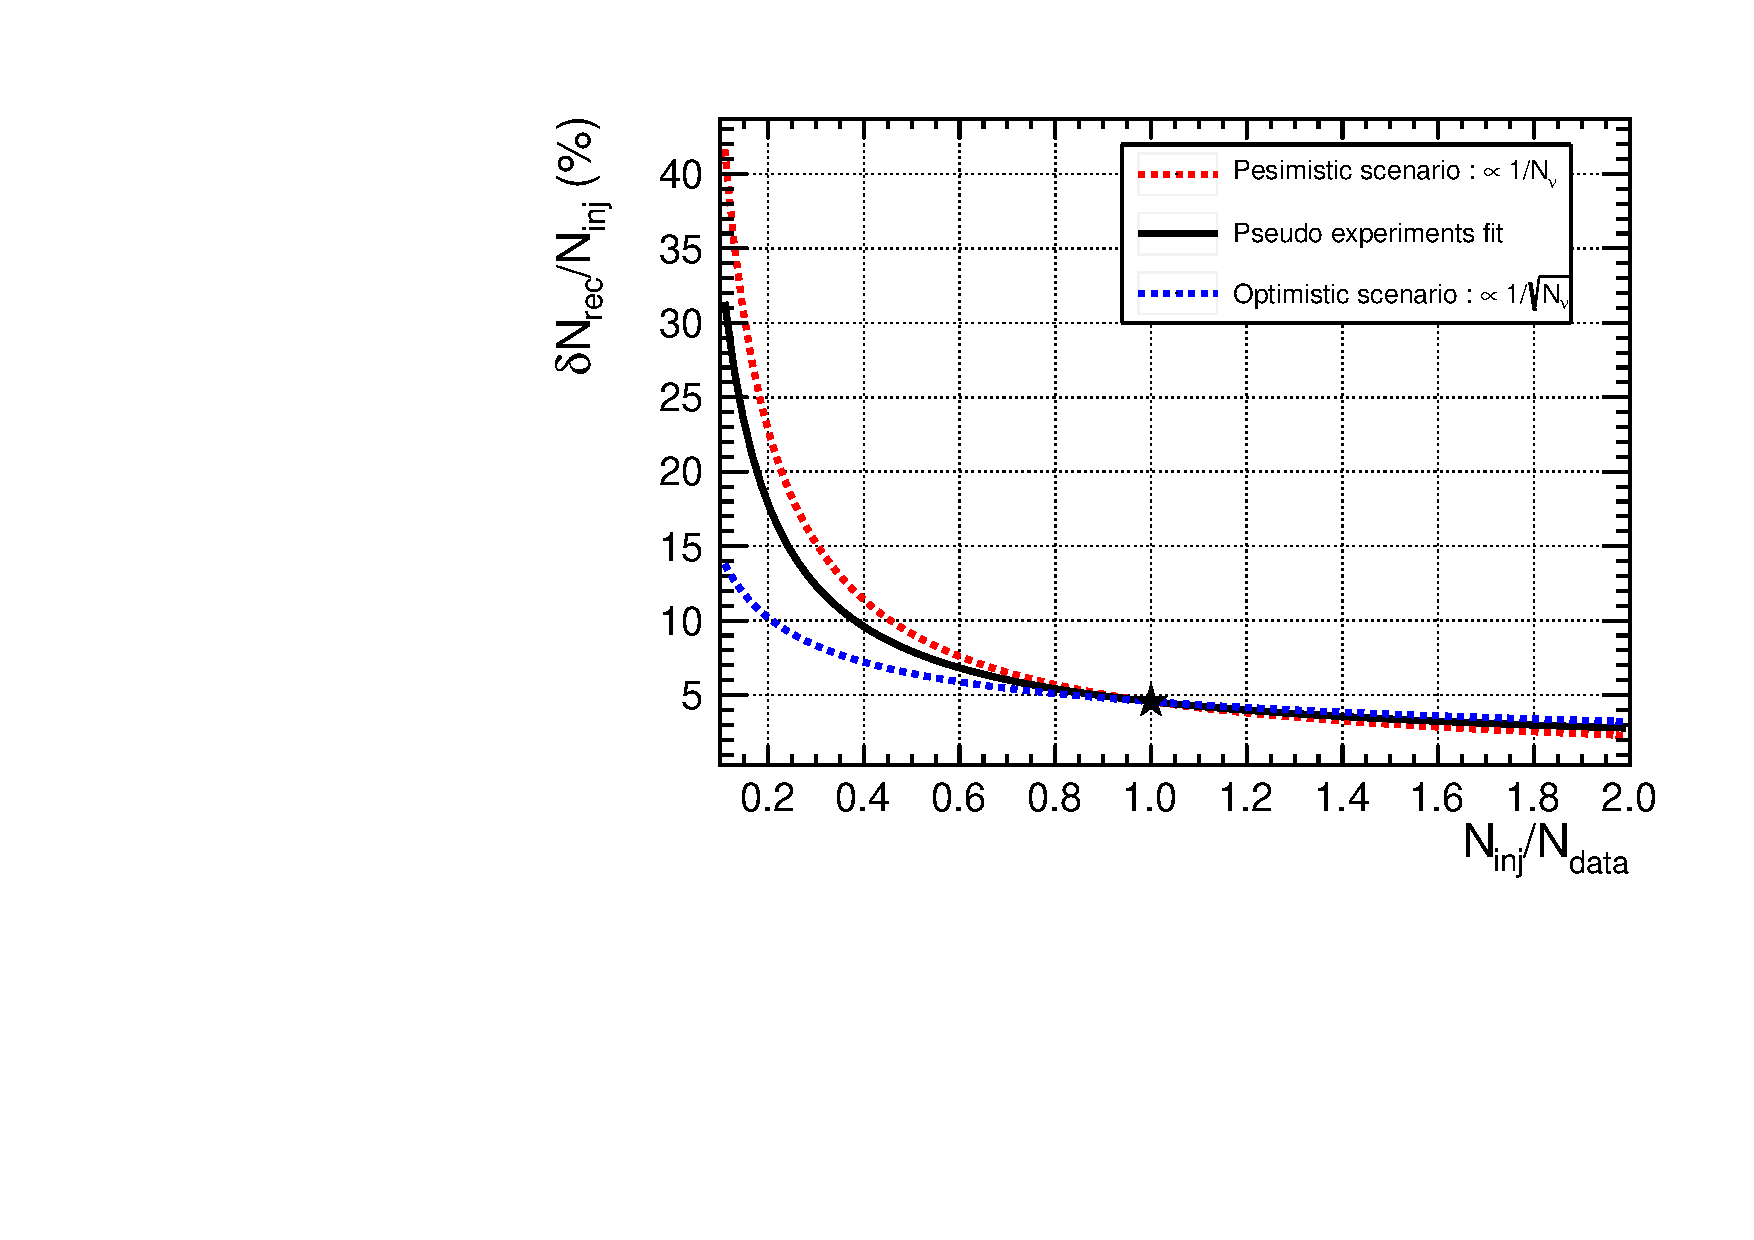
\includegraphics[width=0.8\linewidth]{images/nu_error_fit.pdf}
\caption[Modèle d'évolution de l'erreur statistique ajusté sur les pseudo-expériences]{Modèle d'évolution de l'erreur statistique ajusté sur les pseudo-expériences (noir). Celle-ci est la combinaison de deux modèles d'évolution: un optimiste en $1/\sqrt{R}$ (pointillé rouge), et un pessimiste $\propto 1/R$, où $R$ est le rapport des taux de comptage $N_\textrm{inj}/N_\textrm{data}$. Ce modèle d'évolution correspond au bin en énergie $[3,625; 4,125]$ de la cellule 1.}
\label{fig:nu_error_fit.pdf}

\end{figure}

\begin{figure}[h!]

\centering
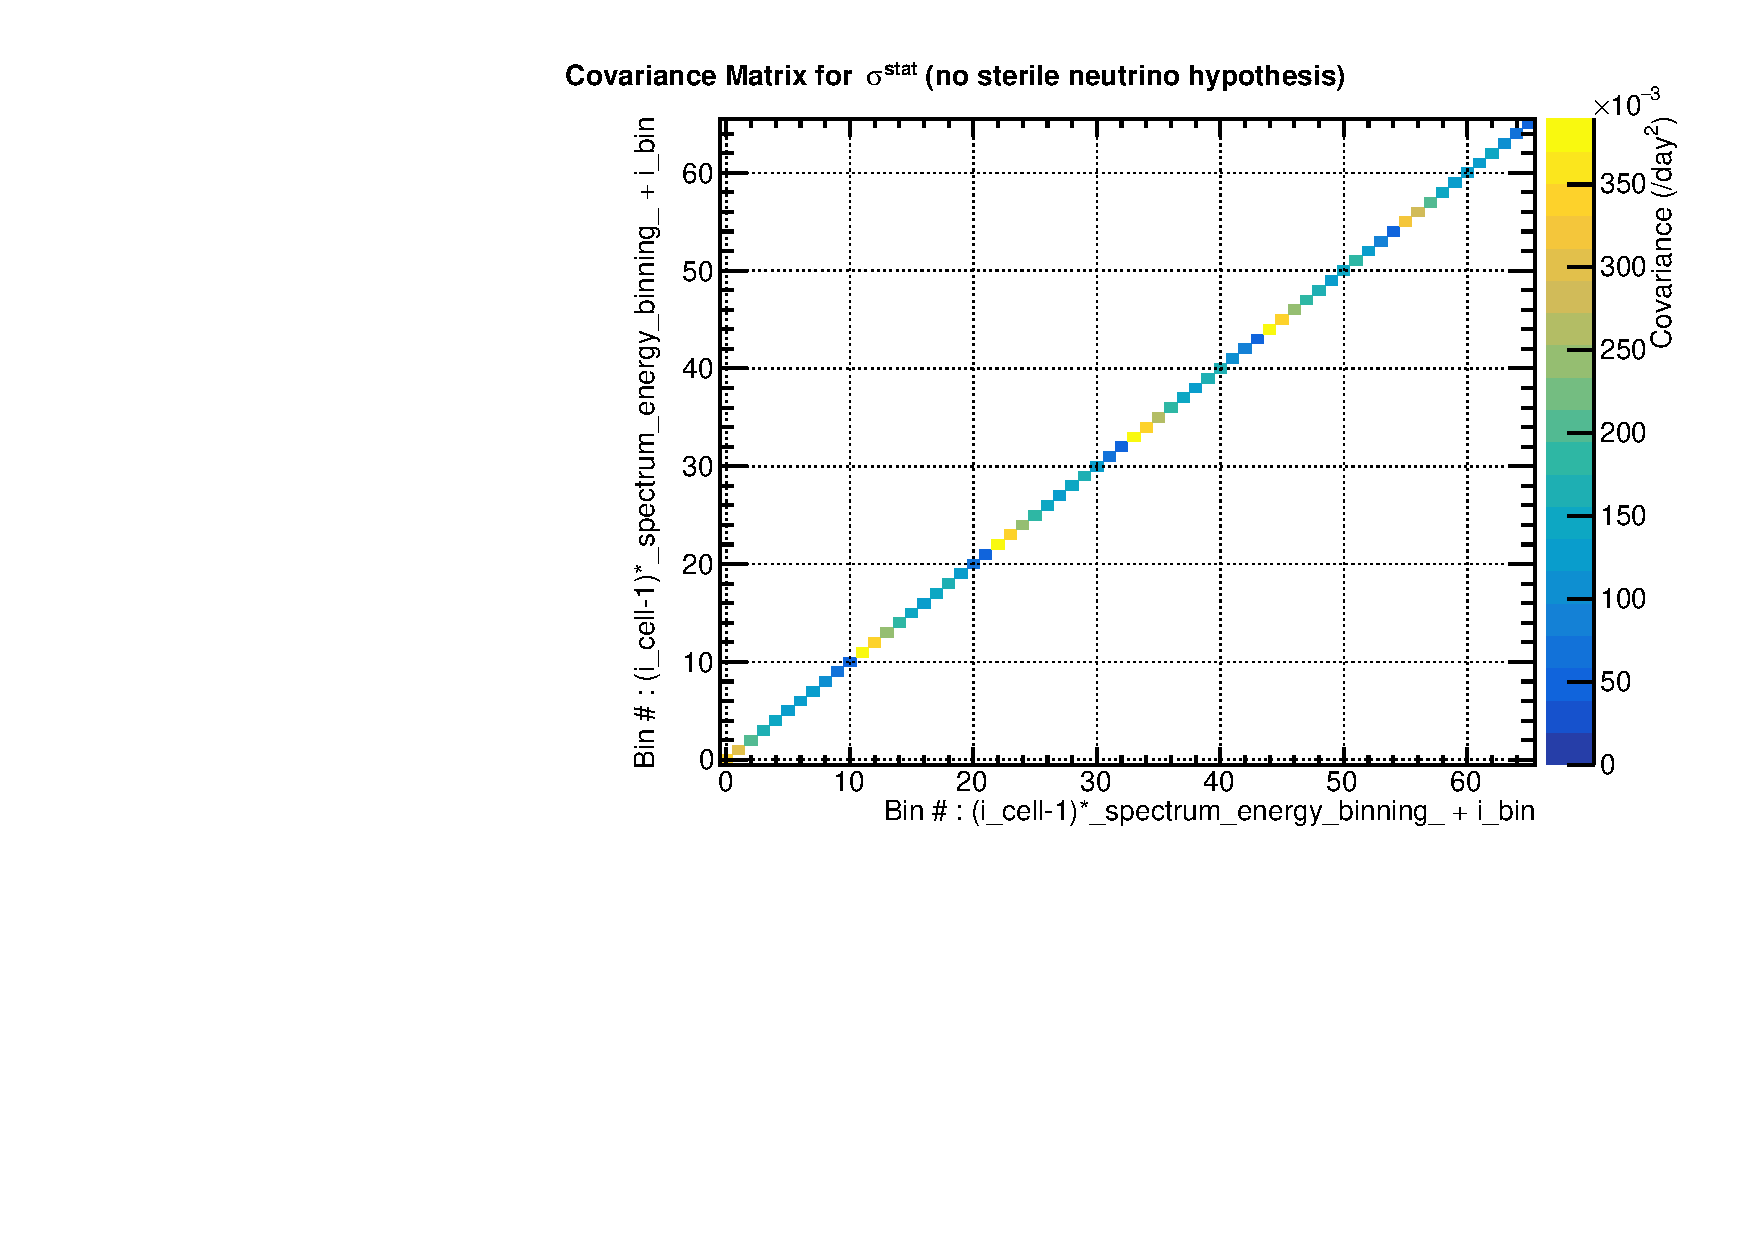
\includegraphics[width=0.8\linewidth]{images/stat_cov_matrix.pdf}
\caption[Matrice de covariance associée aux erreurs statistiques]{Matrice de covariance associée aux erreurs statistiques. Les bins colorés représentent les composantes non nulles de la matrice. Chaque cellule est disposée l'une derrière l'autre tous les 11 bins (en énergie).}
\label{fig:stat_cov_matrix.pdf}

\end{figure}

\clearpage

% stat_cov_matrix.pdf
%\begin{figure}[h!]
%
%\centering
%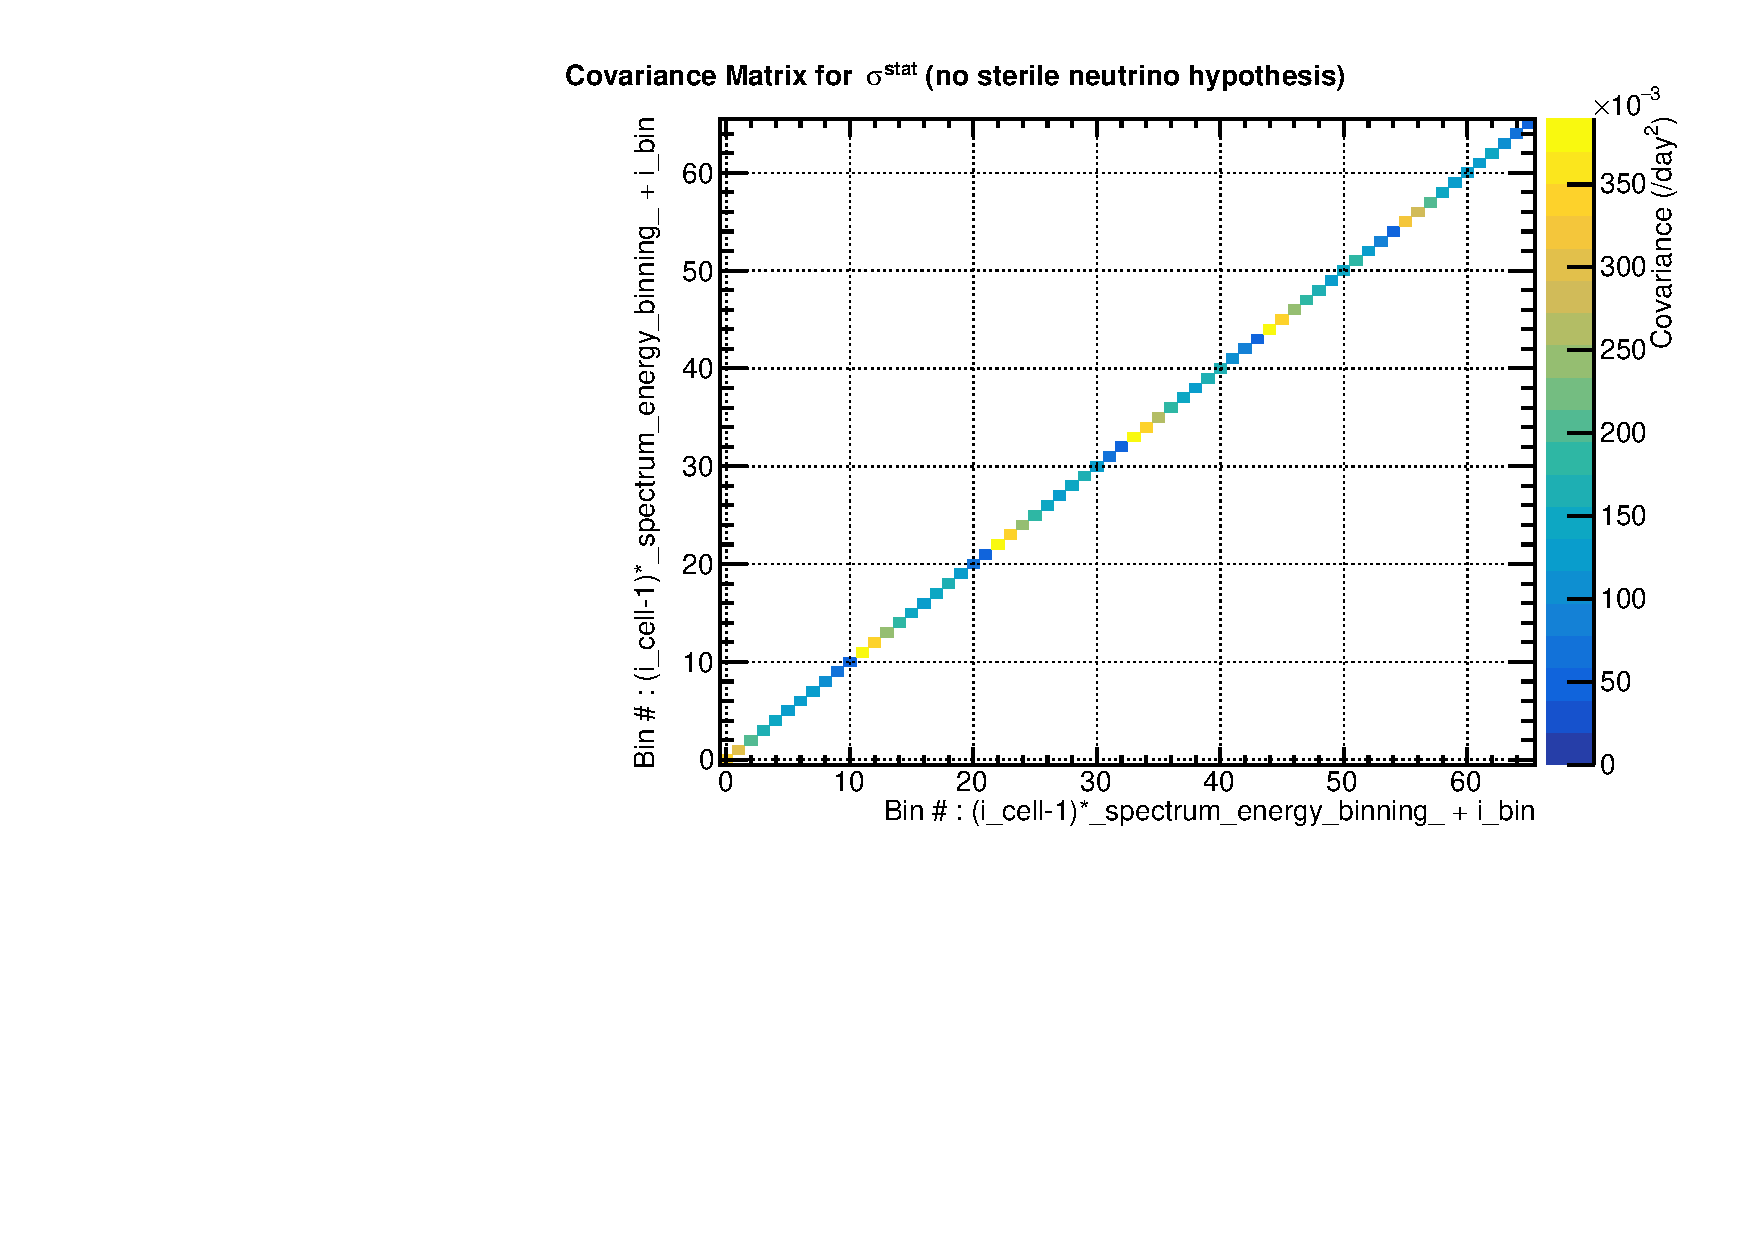
\includegraphics[width=0.9\linewidth]{images/stat_cov_matrix.pdf}
%\caption[Matrice de covariance associée aux erreurs statistiques]{Matrice de covariance associée aux erreurs statistiques. Les bins colorés représentent les composantes non nulles de la matrice. Chaque cellule est disposée l'une derrière l'autre tous les 11 bins (en énergie).}
%\label{fig:stat_cov_matrix.pdf}
%
%\end{figure}





}

Ainsi dans le $\chi^2$, chaque prédiction $M_{cb}$ est accompagnée de son erreur statistique $\sigma_{cb}^\textrm{stat}$ en appliquant la formule (\ref{eq:stat_error}). En pratique, la valeur de $R$ est choisie en prenant le rapport des prédictions : $R = M_{cb}(\Delta m^2_{14}, \textrm{sin}^2(2\theta_{14}))/M_{cb}(\textrm{3 neutrinos})$. Cela signifie que lorsque $R=1$, l'erreur statistique est celle associée aux taux de comptage des données. C'est pourquoi, bien que le $\chi^2$ utilisé pour l'analyse des oscillations est en apparence complètement indépendant de la normalisation (cf. Section \ref{sec:lediberder_chi2}), cet \textit{a priori} sur l'évolution des barres d'erreurs considère implicitement le choix d'une échelle absolue. D'autre part, cette convention implique que les barres d'erreurs associées aux  données correspondent au scénario sans neutrino stérile. En effet, si les données sont atténuées par l'effet d'une oscillation vers un neutrino stérile, l'erreur statistique associée à la prédiction est sous-estimée. Cela dit, la région d'intérêt de l'anomalie concernant des angles de mélange à $\sim 10 \%$, le biais sur l'erreur statistique resterait faible.\\

Étant donné que la reconstruction du taux de comptage $D_{cb}$ est effectuée dans chaque cellule et chaque bin en énergie indépendamment des autres, la matrice de covariance associée à l'erreur statistique est diagonale:

\begin{equation}
    \left[V_\textrm{cov}^\textrm{stat}\right]_{cb,c'b'} = \sigma_{cb}^\textrm{stat} \sigma_{c'b'}^\textrm{stat} \delta_{cc'}\delta_{bb'},
\end{equation}

\bigbreak

où $\delta_{cc'}$ et $\delta_{bb'}$ sont les symboles de Kronecker. La matrice de covariance $V_\textrm{cov}^\textrm{stat}$ est illustrée sur la figure \ref{fig:stat_cov_matrix.pdf}.

\bigbreak

\subsection{Propagation des incertitudes sur l'échelle en énergie : $\sigma^{EU}$ et $\sigma^{EC}$}
\label{sec:Escal_propagation_linear_for_chi2}

Les incertitudes sur l'échelle en énergie se propagent sur les spectres mesurés en changeant le contenu d'un bin $M_{cb}$ en fonction de leurs voisins : $M_{cb+1}$ et $M_{cb-1}$. Soit le paramètre de nuisance $\alpha$ traduisant l'amplitude de la distorsion de l'échelle en énergie:

\begin{equation}
\label{eq:escale_distorsion_firstorder}
    E' = E(1 + \alpha ).
\end{equation}

\bigbreak

La différence entre le contenu du bin $M_{cb}'$ sur l'échelle $E'$ et $M_{cb}$ sur l'échelle originale $E$ peut être exprimée à l'aide de la densité de probabilité du spectre positron mesuré $m(E)$:

\begin{equation}
    \Delta M_{cb}(\alpha) \doteq M'_{cb} - M_{cb} = \int_{E'^-_b}^{E'^+_b} m'(E')dE' - \int_{E^-_b}^{E^+_b} m(E)dE,
\end{equation}

où $E^{\pm}_b$ et $E'^{\pm}_b$ sont les bornes en énergie du bin $b$. Puisque $m$ et $m'$ expriment le même spectre continu sur des échelles différentes, la relation suivante est vraie: $m(E)dE = m'(E')dE'$. Ainsi, $\Delta M_{cb}$ devient:

\begin{equation}
    \Delta M_{cb} = \int_{\frac{E^-}{1+\alpha}}^{E^-} m(E)dE - \int_{\frac{E^+}{1+\alpha}}^{E^+} m(E)dE.
\end{equation}

\bigbreak

En considérant $\alpha > 0$, l'intégrale sur $E^-$ représente le nombre de neutrinos récupérés du bin précédent $b-1$, et $E^+$ le nombre transmis au bin suivant $b+1$. Comme $\alpha$ est supposé faible ($\alpha \ll 1$), les intégrales peuvent être approximées:

\begin{equation}
    \Delta M_{cb} \simeq \alpha\left( m(E^-)E^- - m(E^+)E^+ \right) + \mathcal{O}(\alpha^2).
\end{equation}

\bigbreak

N'ayant pas accès au spectre $m(E)$, les valeurs $m(E^\pm)$ sont approchées par le contenu des bins $b$ et $b \pm 1$:

\begin{equation}
    m(E^\pm) \simeq \frac{M_{cb} + M_{cb\pm 1}}{2} \frac{1}{(E^+ - E^-)} .
\end{equation}

\bigbreak

où $(E^+ - E^-)$ exprime la largeur du bin $M_{cb}$. Ainsi, la valeur de $\Delta M_{cb}$ est obtenue à partir d'un spectre binné $M_{cb}$ avec:

\begin{equation}
    \Delta M_{cb} = \alpha \left(\frac{(M_{cb} + M_{cb-1})E^- - (M_{cb} + M_{cb+1})E^+}{2(E^+ - E^-)} \right) \doteq \alpha \Delta \eta_{cb}
\end{equation}

\bigbreak

Une déformation sur les spectres s'écrit donc : $M_{cb} = \overline{M}_{cb} + \alpha \Delta \eta_{cb}$, où $\overline{M}_{cb}$ est le spectre des données Asimov. Il est important de noter que l'expression de $\Delta M_{cb}$ fait intervenir le contenu des bins en énergie $b\pm 1$. Pour propager correctement cette incertitude, les spectres $M_{cb}$ ont été générés en ajoutant deux bins supplémentaires : un avant le premier et un après le dernier. Ces expressions analytiques ont été validées en simulant deux spectres neutrinos avec des calibrations différentes.\\

Des études sont en cours pour traiter le cas général d'une distorsion quelconque de l'échelle en énergie, au-delà du simple terme linéaire. Cette étude a pour but de chiffrer, à l'aide d'un fit global, l'enveloppe des distorsions possibles à l'intérieur de toutes les contraintes expérimentales de calibration (sources radioactives et $\ce{^{12}B}$). L'impact sur la forme du spectre neutrino est alors calculé avec le formalisme de l'article de G. Mention \cite{Mention:2017dyq}. Cet aspect est brièvement discuté dans les perspectives du Chapitre \ref{chap:chapitre_results}.

% Discuter aussi le traitement en cours du cas général d'une distorsion quelconque de l'énergie scale, au-delà du simple terme linéaire. Cette étude a pour but de chiffrer, à l'aide d'un fit global, l'enveloppe des distortions possibles à l'intérieur de toutes les contraintes expérimentales de calibration (sources radioactives et 12B). L'impact sur la forme du spectre neutrino est alors calculé avec le formalisme de l'article de G. Mention (à citer en ref.).

%D'autre part, on remarquera que cette expression peut être généralisée à une déformation variable sur l'échelle en énergie $\alpha(E)$. Tant que $\alpha(E)$ reste faible devant 1, $\Delta M_{cb}$ s'écrit:
%
%\begin{equation}
%    \Delta M_{cb}(\alpha(E)) = \alpha(E^-) \frac{(M_{cb} + M_{cb-1})E^-}{2(E^+ - E^-)} - \alpha(E^+) \frac{(M_{cb} + M_{cb+1})E^+}{2(E^+ - E^-)}.
%\end{equation}

\bigbreak

L'échelle d'amplitude des paramètres de nuisances $\alpha^{EC}$ et $\alpha_c^{EU}$ est donnée par l'incertitude systématique sur l'échelle en énergie ($\sigma^{EC}$ ou $\sigma^{EU}$), présentée dans la Section \ref{sec:estimation_escale_errors}. Puisque les paramètres $\alpha^{EC}$ et $\alpha^{EU}$ ne sont pas exprimés dans la base du $\chi^2$ ($D_{cb} - \phi_bM_{cb}$), la transformation à l'aide des Jacobiennes est nécessaire (cf. Équation \ref{eq:covariance_basis_change}). Dans leur base propre, les matrices de covariance ont la forme :

\begin{equation}
\begin{gathered}
    V_\textrm{cov}^{EC}\left(\alpha^{EC}\right) = (\sigma^{EC}),\\
    V_\textrm{cov}^{EU}\left(\alpha^{EU}_c\right) = \left(\begin{matrix}
        \sigma^{EU} & 0 & 0 & 0 & 0 & 0 \\
        0 & \sigma^{EU} & 0 & 0 & 0 & 0 \\
        0 & 0 & \sigma^{EU} & 0 & 0 & 0 \\
        0 & 0 & 0 & \sigma^{EU} & 0 & 0 \\
        0 & 0 & 0 & 0 & \sigma^{EU} & 0 \\
        0 & 0 & 0 & 0 & 0 & \sigma^{EU} \\
    \end{matrix} \right).
\end{gathered}
\end{equation}

\bigbreak

$V_\textrm{cov}^{EC}$ est une matrice 1x1, car il n'y a qu'un seul $\alpha^{EC}$ commun pour toutes les cellules, tandis que $V_\textrm{cov}^{EU}$ est une matrice 6x6 pour chaque $\alpha^{EU}_c$. Pour changer de base, les Jacobinnes sont calculées :

\begin{equation}
\begin{gathered}
    \left[J^{EC}\right]_{cb,1} = \frac{\partial \left(\phi_bM_{cb}\right)}{\partial \alpha^{EC}} = \phi_b \frac{\partial \left(\overline{M}_{cb} + \alpha^{EC} \Delta \eta_{cb}\right)}{\partial \alpha^{EC}} = \phi_b \Delta \eta_{cb},\\
    \left[J^{EU}\right]_{cb,c^*} = \frac{\partial \left(\phi_bM_{cb}\right)}{\partial \alpha^{EU}_{c^*}} = \phi_b \frac{\partial \left(\overline{M}_{cb} + \alpha^{EU}_c \Delta \eta_{cb}\right)}{\partial \alpha^{EU}_{c^*}} = \phi_b \delta_{cc^*} \Delta \eta_{cb}.
\end{gathered}
\end{equation}

\afterpage{

\begin{figure}[h!]
\centering
\begin{subfigure}[b]{0.49\textwidth}
\centering
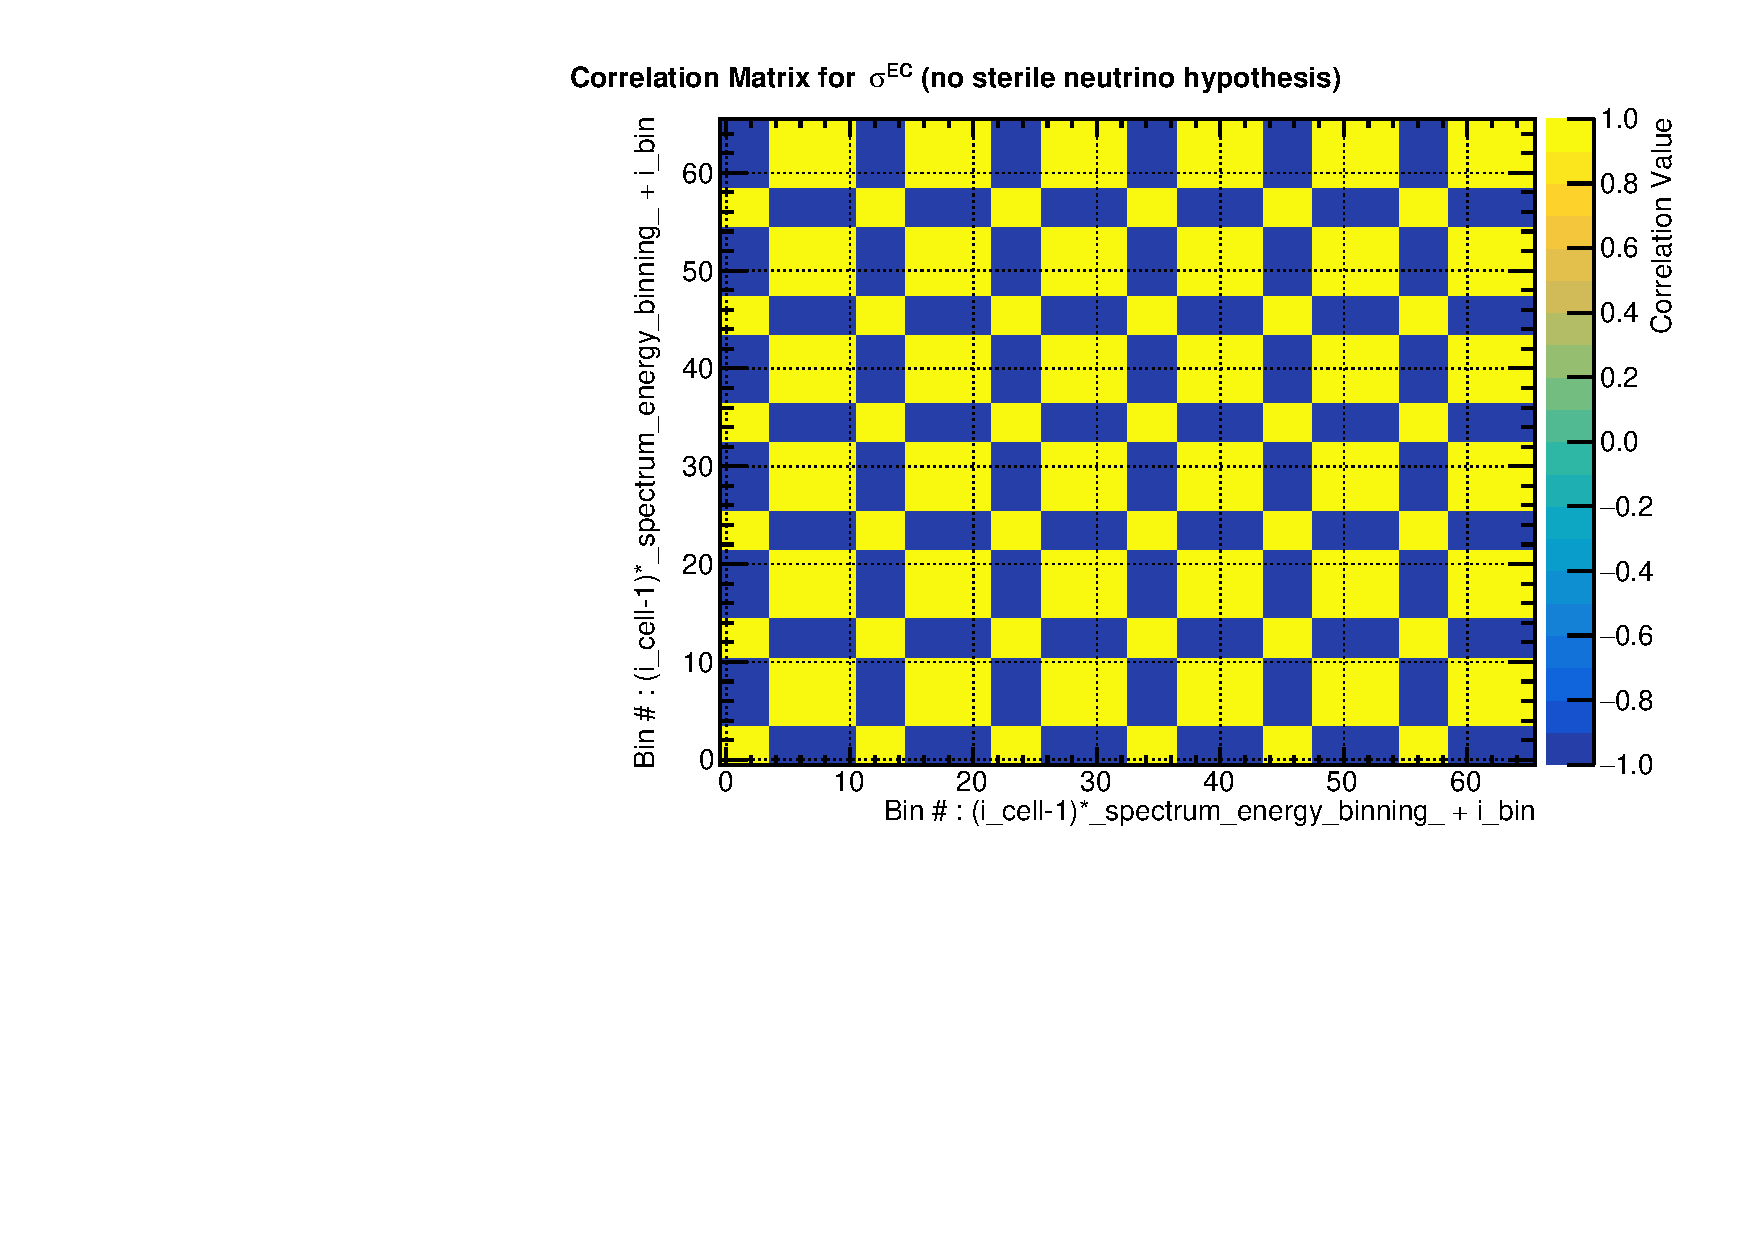
\includegraphics[width=1\textwidth]{images/EC_corr_matrix.pdf}
\caption{Erreur sur l'échelle en énergie corrélée sur toutes les cellules : $\sigma^{EC}$.}
\label{fig:EC_corr_matrix.pdf}
\end{subfigure}
~ % attention ! space sensitive
\begin{subfigure}[b]{0.49\textwidth}
\centering
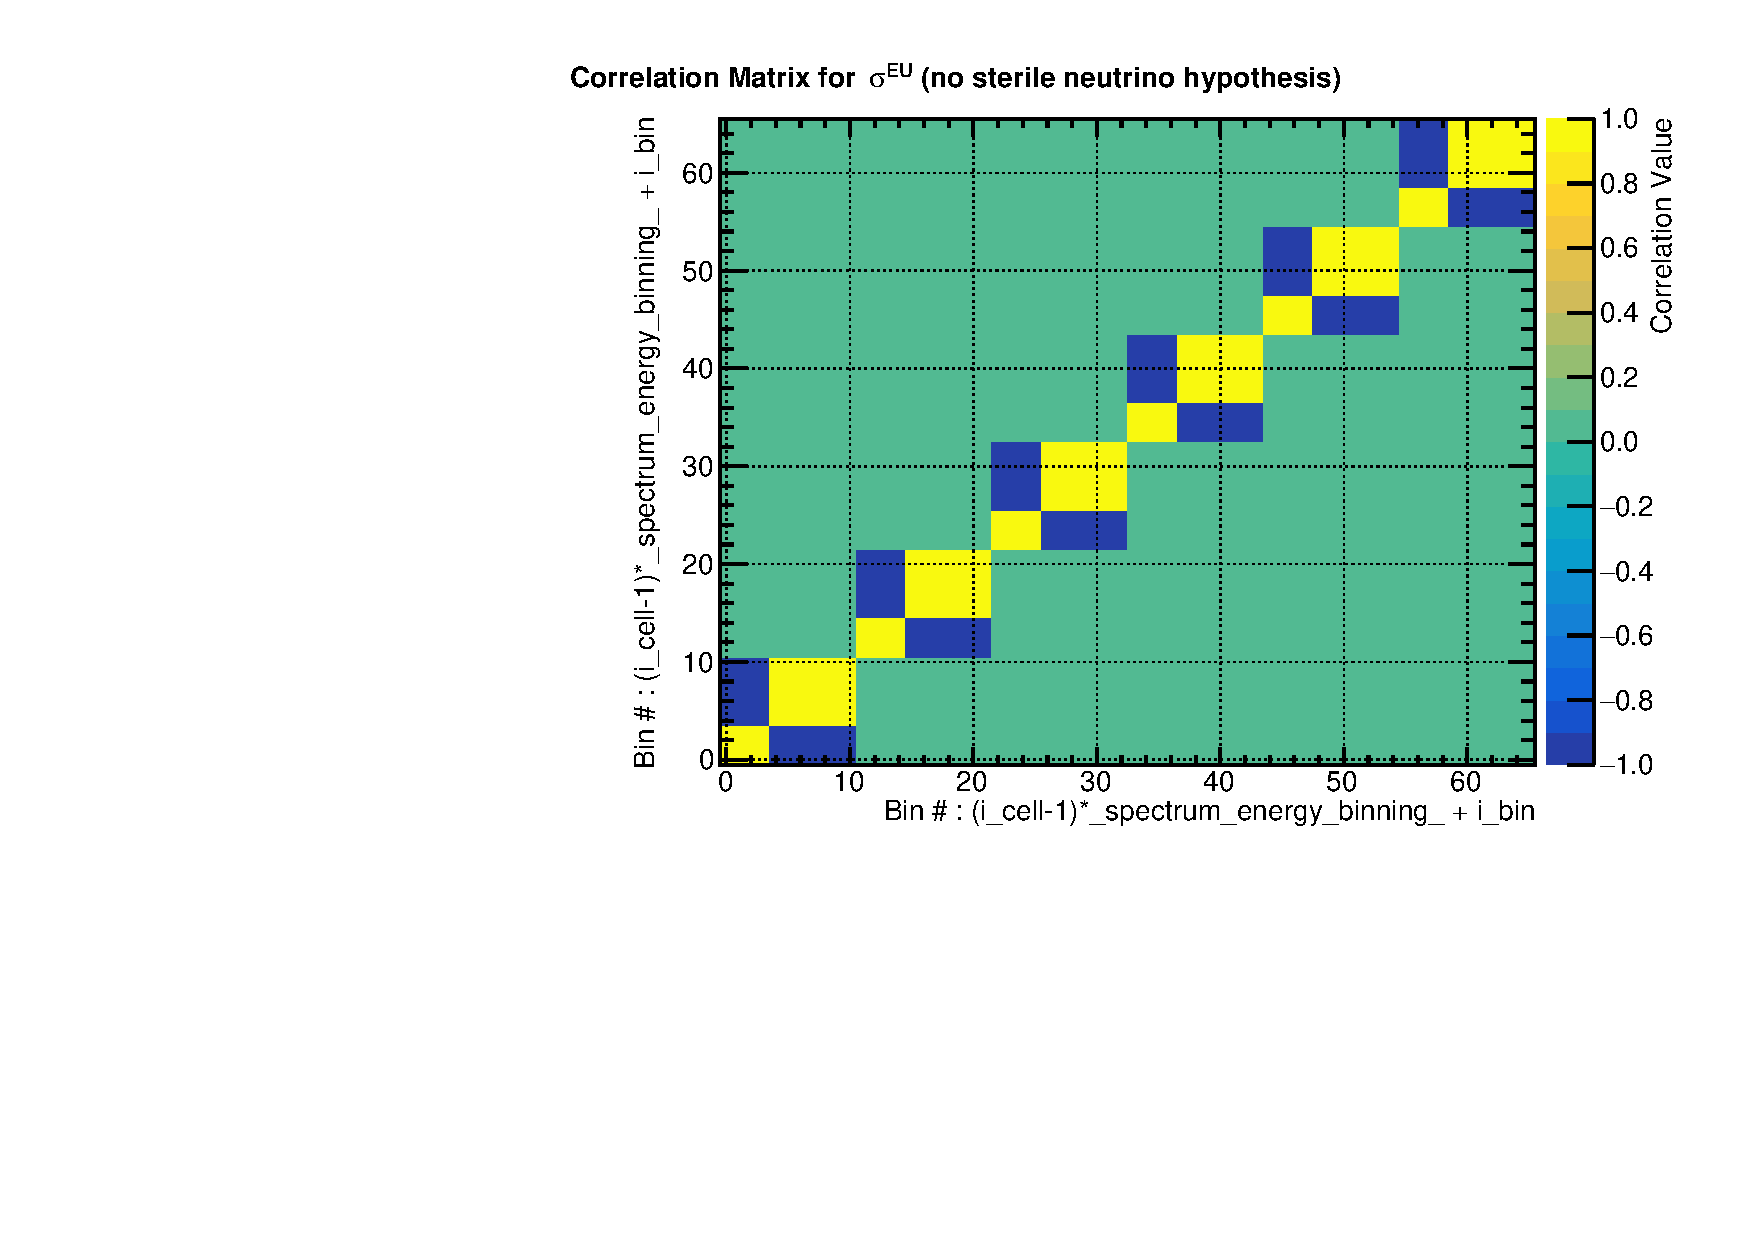
\includegraphics[width=1\textwidth]{images/EU_corr_matrix.pdf}
\caption{Erreur sur l'échelle en énergie décorrélée cellules à cellule : $\sigma^{EU}$.}
\label{fig:EU_corr_matrix.pdf}
\end{subfigure}
\caption[Matrices de corrélations associées aux incertitudes sur l'échelle en énergie]{Matrices de corrélations associées aux incertitudes sur l'échelle en énergie. Chaque cellule est disposée l'une derrière l'autre tous les 11 bins (en énergie).}
\label{fig:EScale_corr_matrix.pdf}
\end{figure}


\begin{figure}[h!]
\centering
\begin{subfigure}[b]{0.49\textwidth}
\centering
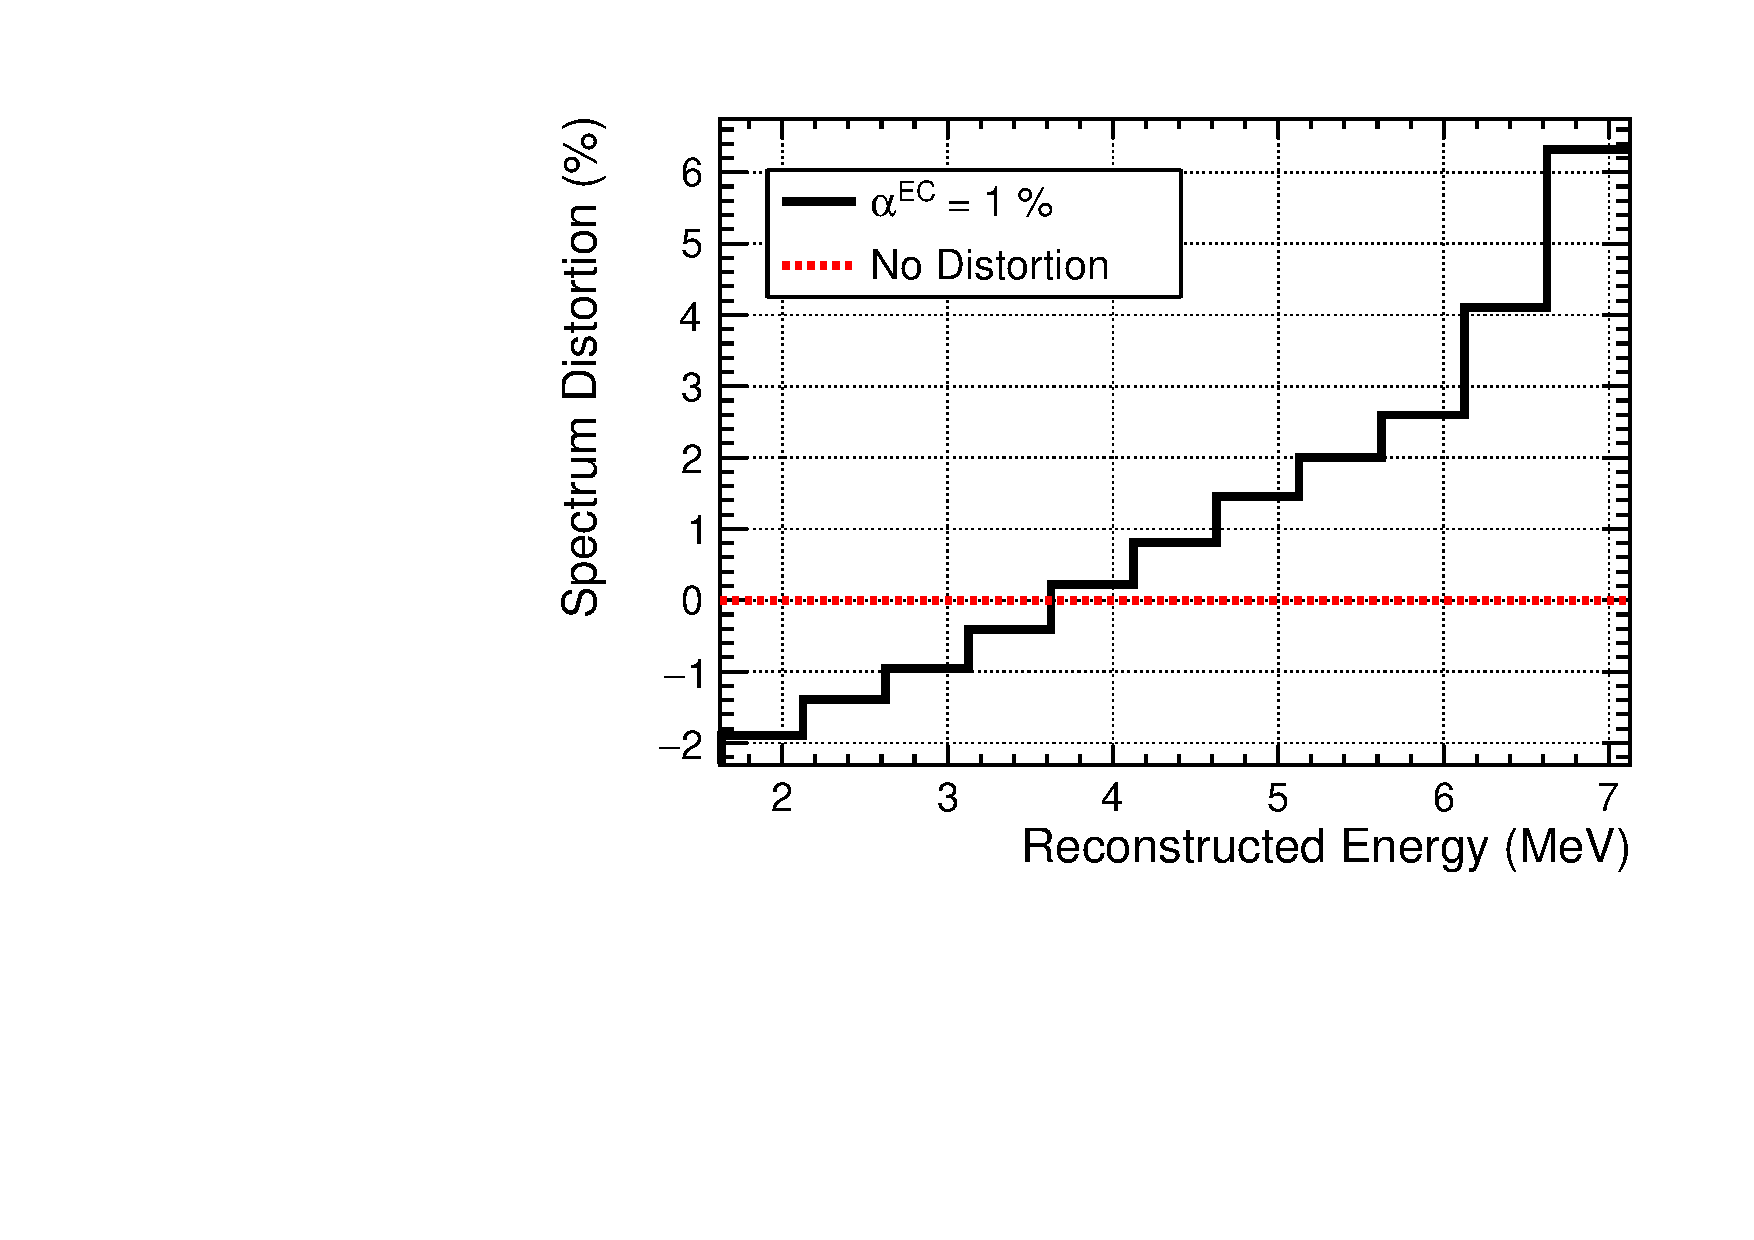
\includegraphics[width=1\textwidth]{images/Escale_distortion_relat.pdf}
\caption{Évolution du rapport $\frac{\alpha^{EC}\Delta \eta_{cb}}{\overline{M}_{cb}}$.}
\label{fig:Escale_distortion_relat.pdf}
\end{subfigure}
~ % attention ! space sensitive
\begin{subfigure}[b]{0.49\textwidth}
\centering
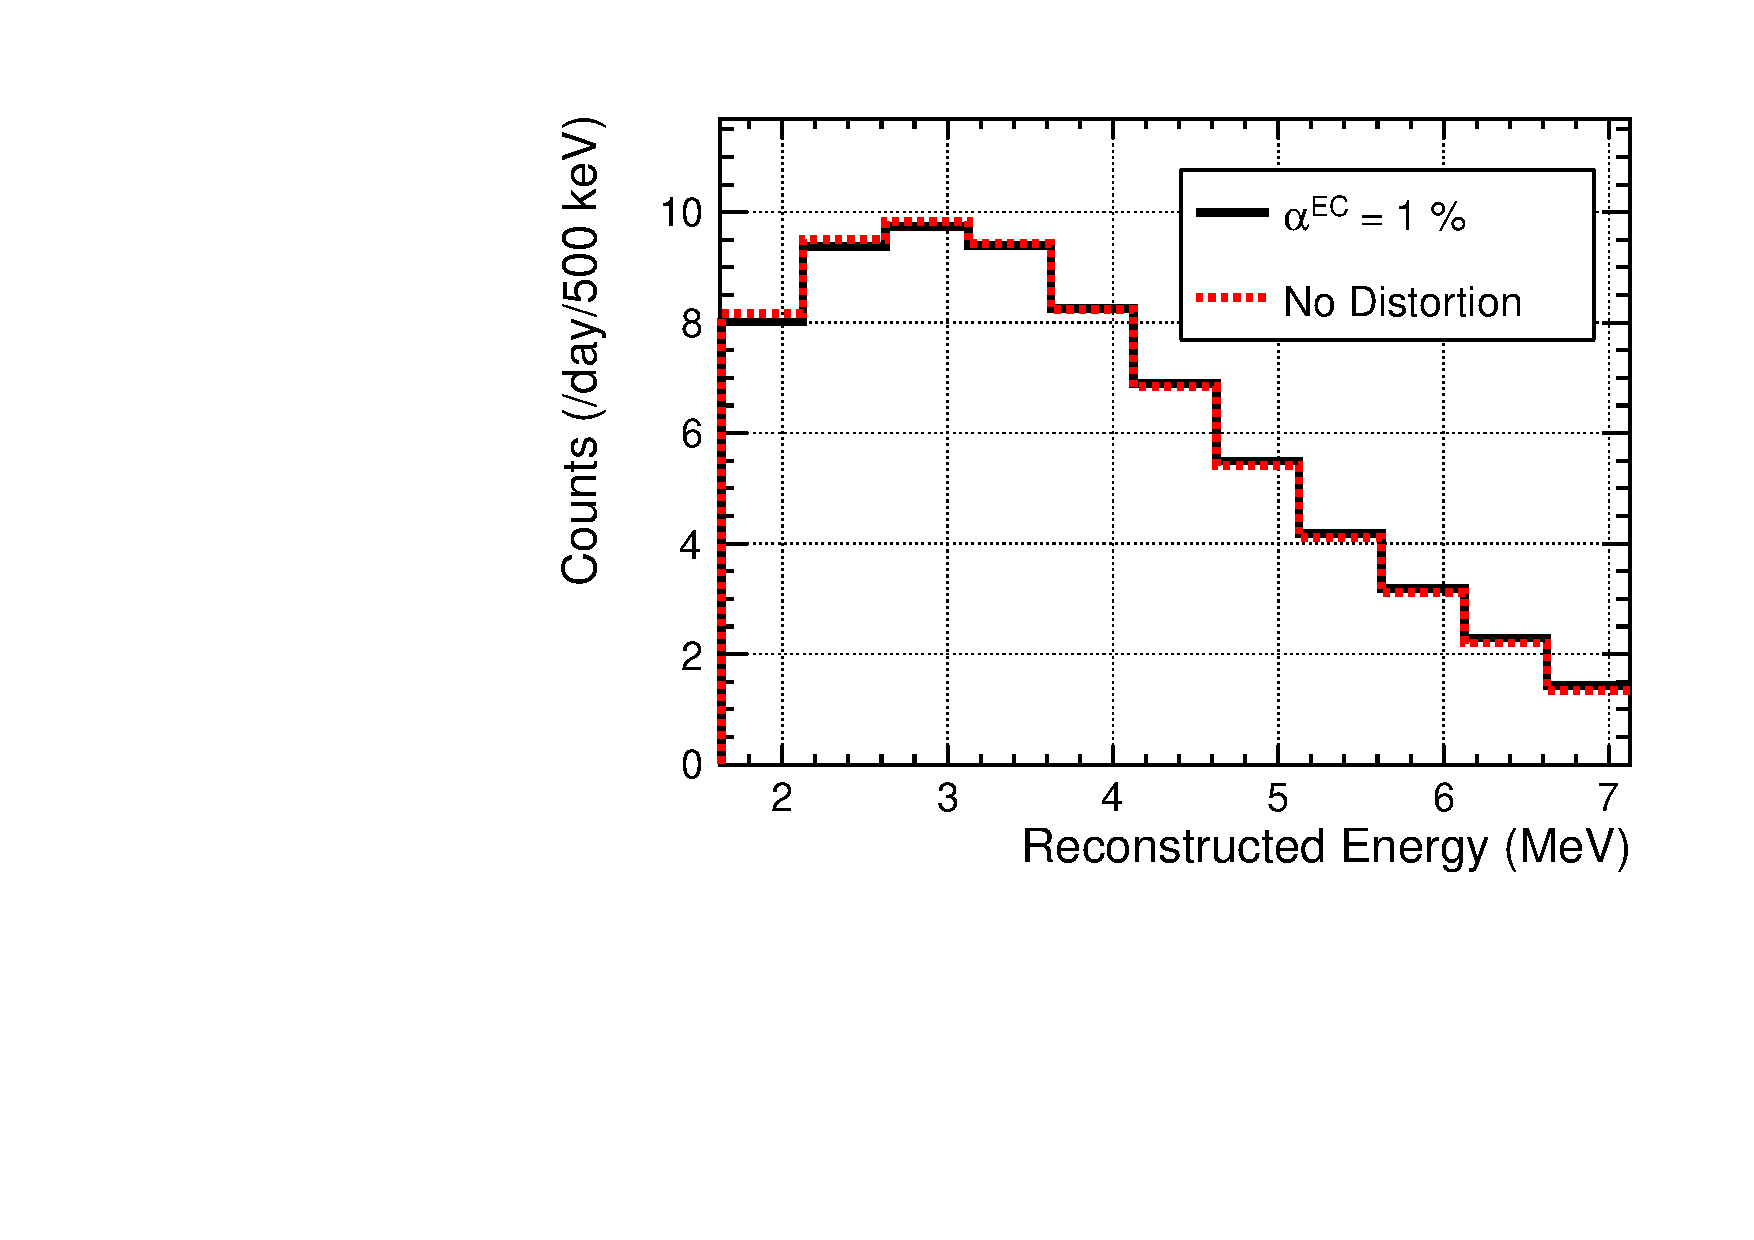
\includegraphics[width=1\textwidth]{images/Escale_distortion_abs.pdf}
\caption{Comparaison des de la forme des spectres avec et sans distorsion : $M_{cb} = \overline{M}_{cb} + \alpha^{EC}\Delta \eta_{cb}$.}
\label{fig:Escale_distortion_abs.pdf}
\end{subfigure}
\caption[Propagation d'une distorsion de l'échelle en énergie sur les spectres positron]{Propagation d'une distorsion de l'échelle en énergie sur les spectres positron. L'amplitude de variation est conduite par le paramètre $\alpha^{EC}$ ($E' = E(1+\alpha^{EC})$) et a été arbitrairement choisie à $2\%$ (noir). Le cas sans distorsion est marqué par les lignes en pointillés rouges.}
\label{fig:EScale_distortion_spectrum}
\end{figure}

}

\bigbreak

Enfin, les matrices de covariance dans la base du $\chi^2$ sont obtenues par l'opération suivante :

\begin{equation}
\begin{gathered}
    \left[V_\textrm{cov}^{EC}\left(\chi^2\right)\right]_{cb,c'b'} = \left[J^{EC}\right]_{cb,1} \sigma^{EC} \left[J^{EC}\right]^\textrm{t}_{1,c'b'}, \\
     \left[V_\textrm{cov}^{EU}\left(\chi^2\right)\right]_{cb,c'b'} = \sum_{c^*} \left[J^{EU}\right]_{cb,c^*} \sigma^{EU} \left[J^{EU}\right]^\textrm{t}_{c^*,cb}.
\end{gathered}
\end{equation}

\bigbreak

À titre d'illustration, les matrices de corrélations\footnote{Les matrices de corrélations sont définies comme la renormalisation de la matrice de covariance par ses termes diagonaux : $\left[V_\textrm{corr}\right]_{ij} \doteq \left[V_\textrm{cov}\right]_{ij}\left/\sqrt{\left[V_\textrm{cov}\right]_{ii} \left[V_\textrm{cov}\right]_{jj}}\right.$.} sont présentées sur la figure \ref{fig:EScale_corr_matrix.pdf}. Dans le cas de $\sigma^{EC}$, les corrélations sont soit 1 soit -1, car les déformations sont toutes engendrées par un seul coefficient. Par ailleurs, le signe $\pm$ est fonction de la pente du spectre : si la pente est positive au bin $i$ et qu'elle est négative au bin $j$, les termes $\Delta M_{cb}$ sont de signe opposé. À l'inverse, la matrice de corrélation associée à $\sigma^{EU}$ présente quelques termes nuls. En effet, puisque les $\alpha^{EU}_{c}$ n'ont pas d'influence sur la cellule $c' (\neq c)$ la corrélation est nulle.\\

La propagation de ces distorsions sur les spectres $M_{cb}$ est présentée sur la figure \ref{fig:EScale_distortion_spectrum}. En ne considérant qu'un décalage d'1 \% sur l'échelle en énergie, les distorsions sur $M_{cb}$ se distribuent entre -2\% et +6\%. En particulier dans la zone à $\sim \SI{5}{MeV}$, l'amplitude des distorsions se situe entre 1,5\% et 2,5\%. C'est de ce constat qu'est parti G. Mention \textit{et al.} \cite{Mention:2017dyq} pour expliquer l'épaulement à $\SI{5}{MeV}$ mesuré par plusieurs expériences neutrinos.

%En effet, en généralisant l'Équation (\ref{eq:escale_distorsion_firstorder}), il est possible d'introduire des distorsions locales sur le spectre:
%
%\begin{equation}
%\begin{gathered}
%    E' = E(1 + \alpha(E)),\\
%    \frac{m'(E')}{m(E)} = 1 - \alpha(E)\left( 1 + \frac{E}{m(E)}\frac{\partial m(E)}{\partial E}\right) - E \frac{\partial \alpha(E)}{\partial E}.
%\end{gathered}
%\end{equation}

\bigbreak

Ainsi, pour contraindre les distorsions de spectres, il est nécessaire de contraindre $\alpha (E)$ sur toute l'échelle en énergie. Ce point est brièvement discuté dans la section sur les perspectives de \textsc{Stereo} (Chapitre \ref{chap:chapitre_results}).

\bigbreak

\subsection{Propagation de l'incertitude sur l'efficacité de détection relative : $\sigma^{NU}$}

Bien que la normalisation absolue du MC ne soit pas nécessaire pour l'analyse d'oscillations, l'efficacité de détection relative entre les différentes cellules doit être correctement reproduite par la simulation. L'incertitude sur la normalisation relative $\sigma^{NU}$ est essentiellement portée par deux composantes : l'efficacité de détection du neutron et le volume de détection de chaque cellule.\\

L'incertitude sur le volume de chaque cellule est donnée par le calcul suivant:

\begin{equation}
\begin{gathered}
    V_\textrm{cell} = X_\textrm{cell} \times Y_\textrm{cell} \times Z_\textrm{cell},\\
    \frac{\delta V_\textrm{cell}}{V_\textrm{cell}} = \sqrt{\left(\frac{\delta X_\textrm{cell}}{X_\textrm{cell}}\right)^2 + \left(\frac{\delta Y_\textrm{cell}}{Y_\textrm{cell}}\right)^2 + \left(\frac{\delta Z_\textrm{cell}}{Z_\textrm{cell}}\right)^2}.
\end{gathered}
\end{equation}

\bigbreak

Les dimensions des cellules ont été mesurées lors de l'assemblage du détecteur interne \cite{docdb469}. La dispersion des valeurs obtenues a donné une estimation de l'incertitude. Par ailleurs, les déformations induites par la différence résiduelle de niveau de liquide dans le GC et dans la TG ont été prises en compte. Ces estimations ont été obtenues par des simulations menées par le bureau d'études au CEA \cite{docdb149}. Finalement, l'erreur relative sur le volume de chaque cellule est:

\begin{equation}
    \frac{\delta V_\textrm{cell}}{V_\textrm{cell}} = 0,83\%.
\end{equation}

\bigbreak

Les études d'efficacité de détection du neutron ont été présentées dans la Section \ref{sec:neutrino_biases_eff} (Chapitre \ref{chap:chapitre_analysie}). Avant de considérer l'incertitude sur la norme, les biais d'efficacité de chaque cellule ont été corrigés dans la simulation. Les disparités d'efficacité cellule à cellule sont engendrées par les coefficients $C_\textrm{Gd}^\nu(\textrm{cell})$ répertoriés dans le Tableau \ref{tab:data_mc_gd_fraction_ratios} (Chapitre \ref{chap:chapitre_analysie}). Le spectre de chaque cellule est ainsi renormalisé: $M_{cb} \rightarrow M_{cb} \times C_\textrm{Gd}^\nu(\textrm{cell})$. L'incertitude sur la mesure de ces $C_\textrm{Gd}^\nu(\textrm{cell})$ est ensuite propagée dans la norme. En outre, l'incertitude sur l'efficacité des coupures topologiques de l'événement Retardé est ajoutée au bilan d'erreur sur la norme: $\delta \left<C_\textrm{Retardé} \right>_{\textrm{cells},z}$. Dès lors, $\sigma^{NU}$ prend la forme suivante:

\begin{equation}
    \sigma^{NU} = \sqrt{\left(\frac{\delta V_\textrm{cell}}{V_\textrm{cell}}\right)^2 + \left(\left< \delta C_\textrm{Gd}^\nu(\textrm{cell}) \right>\right)^2 + \left(\delta \left<C_\textrm{Retardé} \right>_{\textrm{cells},z}\right)^2} = 1,2\%. (\footnotemark)
\end{equation}
\footnotetext{Il s'agit de la valeur utilisée pour les résultats présentés à Moriond 2019 \cite{docdb849}. À l'époque la cascade n-Gd était exécutée par GLG4Sim. Ce nombre est donc susceptible de changer avec la mise à jour FIFRELIN.}

\afterpage{

% stat_cov_matrix.pdf
\begin{figure}[h!]

\centering
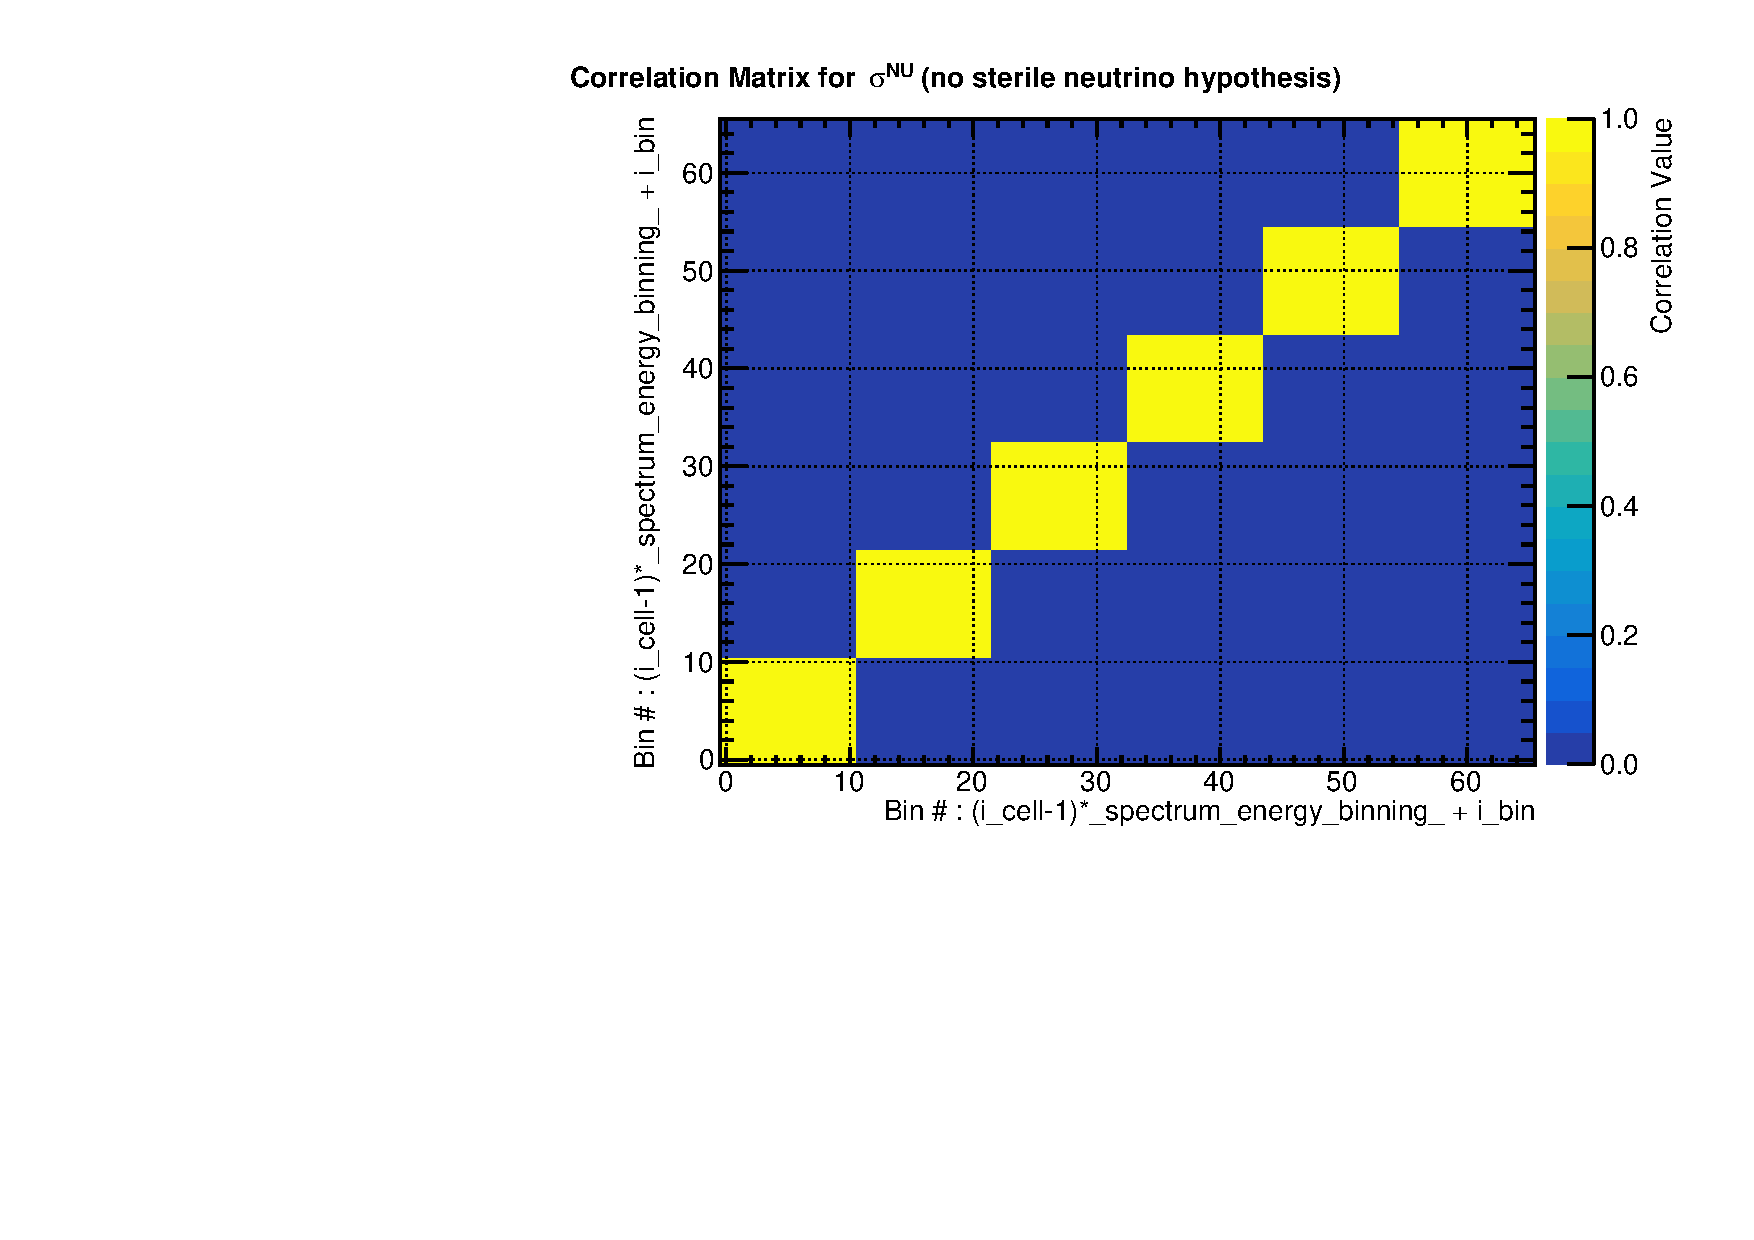
\includegraphics[width=0.9\linewidth]{images/NU_corr_matrix.pdf}
\caption[Matrice de corrélation associée aux erreurs sur la norme relative]{Matrice de corrélation associée aux erreurs sur la norme relative. Les bins colorés représentent les composantes non nulles de la matrice. Chaque cellule est disposée l'une derrière l'autre tous les 11 bins (en énergie).}
\label{fig:NU_corr_matrix.pdf}

\end{figure}

\begin{figure}[h!]

\centering
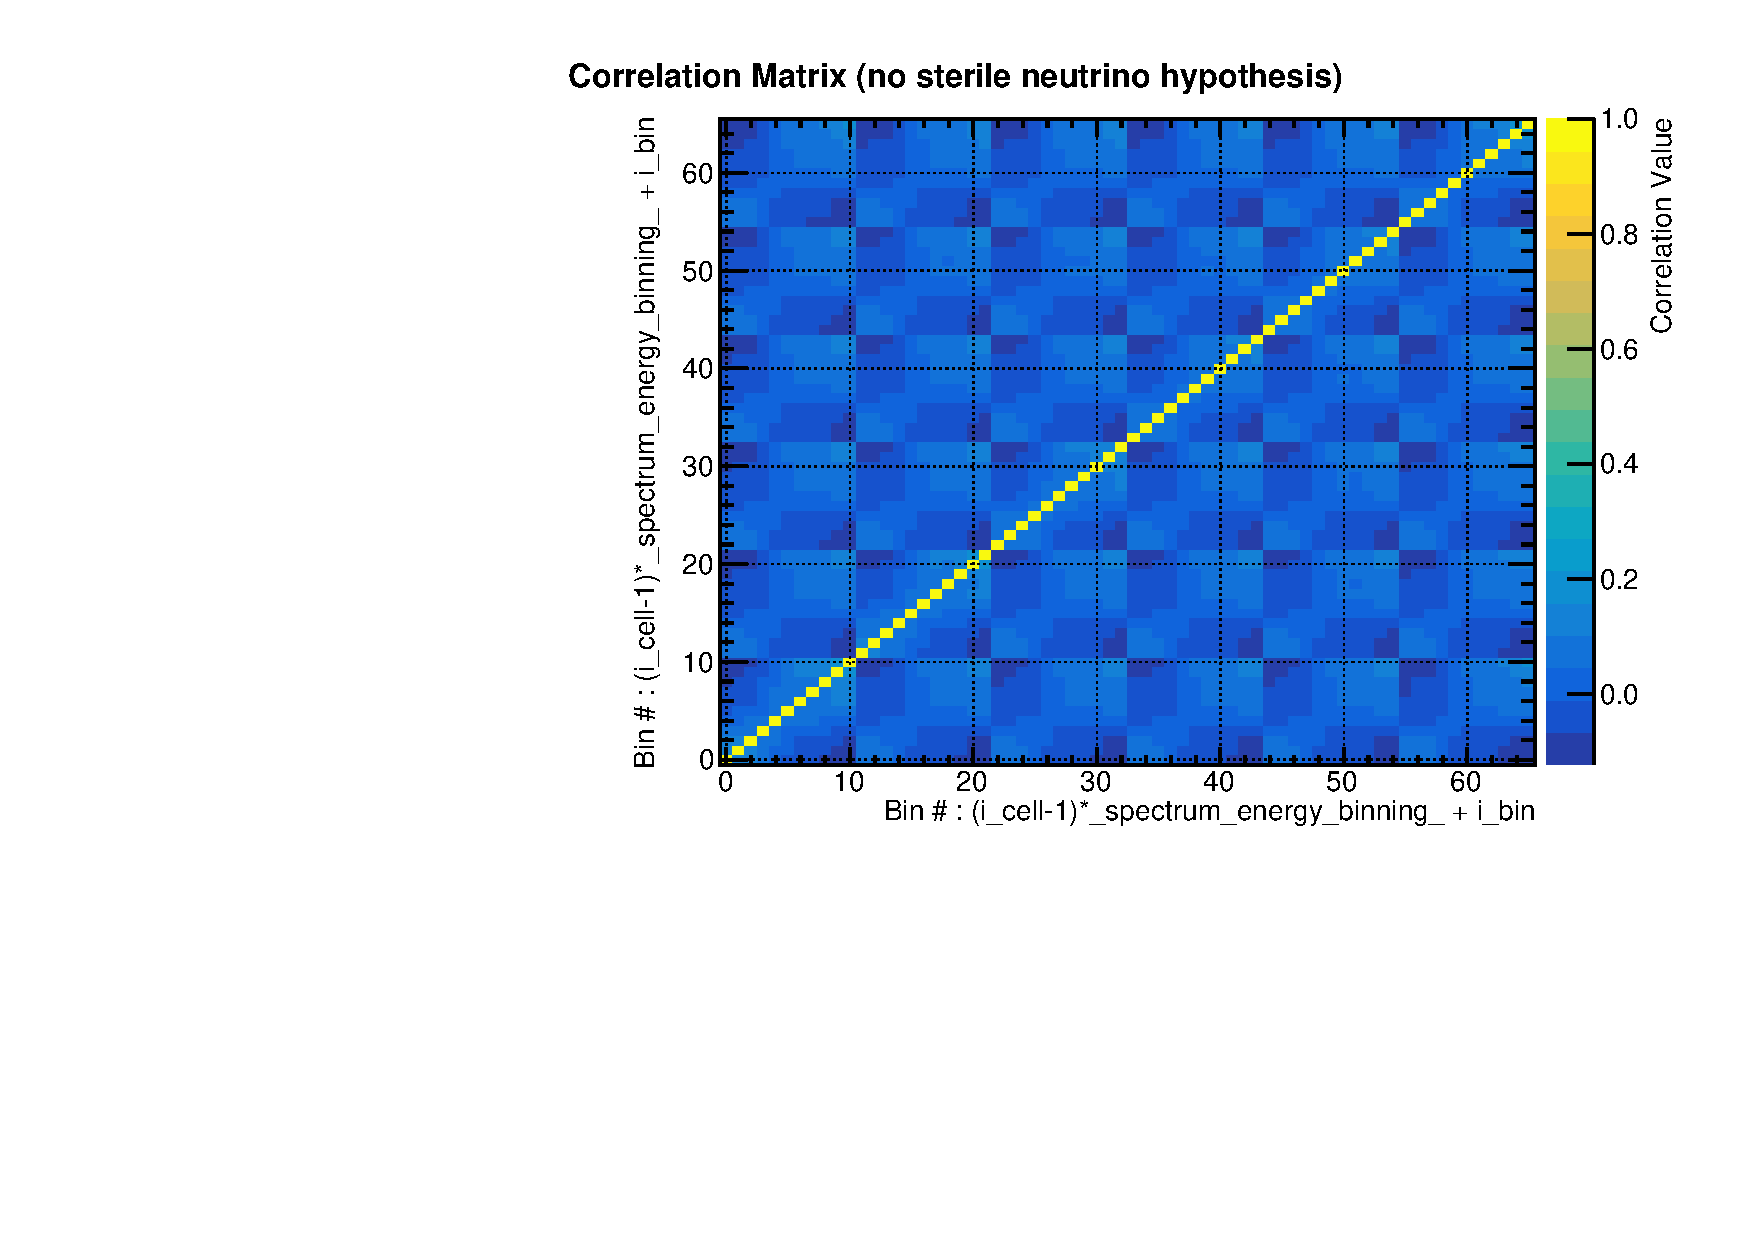
\includegraphics[width=0.9\linewidth]{images/Total_corr_matrix.pdf}
\caption[Matrice de corrélation totale intervenant dans le $\chi^2_\phi$]{Matrice de corrélation totale intervenant dans le $\chi^2_\phi$. Chaque cellule est disposée l'une derrière l'autre tous les 11 bins (en énergie).}
\label{fig:Total_corr_matrix.pdf}

\end{figure}

\clearpage

}

\bigbreak

L'incertitude relative sur la normalisation se propage via six paramètres de nuisance $\alpha^{NU}_c$ (un par cellule), qui affecte les $M_{cb}$ de la sorte :

\begin{equation}
    M_{cb} = \overline{M}_{cb}(1 + \alpha_c^{NU}).
\end{equation}

\bigbreak

Les composantes de la Jacobienne sont déterminées comme pour l'échelle en énergie, et la matrice de covariance dans la base dictée par le $\chi^2$ est calculée de la façon suivante :

\begin{equation}
\begin{gathered}
V_\textrm{cov}^{NU}\left(\alpha^{NU}_c\right) = \left(\begin{matrix}
        \sigma^{NU} & 0 & 0 & 0 & 0 & 0 \\
        0 & \sigma^{NU} & 0 & 0 & 0 & 0 \\
        0 & 0 & \sigma^{NU} & 0 & 0 & 0 \\
        0 & 0 & 0 & \sigma^{NU} & 0 & 0 \\
        0 & 0 & 0 & 0 & \sigma^{NU} & 0 \\
        0 & 0 & 0 & 0 & 0 & \sigma^{NU} \\
    \end{matrix} \right),\\
\left[J^{NU}\right]_{cb,c^*} = \frac{\partial \left(\phi_bM_{cb}\right)}{\partial \alpha^{NU}_{c^*}} = \phi_b \frac{\partial \left(\overline{M}_{cb}(1 + \alpha^{NU}_c)\right)}{\partial \alpha^{NU}_{c^*}} = \phi_b \delta_{cc^*} \overline{M}_{cb},\\
\left[V_\textrm{cov}^{NU}\left(\chi^2\right)\right]_{cb,c'b'} = \sum_{c^*} \left[J^{NU}\right]_{cb,c^*} \sigma^{NU} \left[J^{NU}\right]^\textrm{t}_{c^*,cb}.
\end{gathered}
\end{equation}

\bigbreak

La figure \ref{fig:NU_corr_matrix.pdf} montre finalement que les bins d'une cellule sont tous affectés de la même manière. De plus, le paramètre de nuisance $\alpha^{NU}_c$ n'affecte pas les spectres dans la cellule $c' \neq c$.

\bigbreak

\subsection{Matrice de covariance totale}
\label{seq:incert_propag}

La matrice de covariance qui intervient dans $\chi^2_{\phi}$ est construite en faisant la somme des quatre composantes:

\begin{equation}
    V_\textrm{cov} = V_\textrm{cov}^\textrm{stat} + V_\textrm{cov}^{NU} + V_\textrm{cov}^{EU} + V_\textrm{cov}^{EC}.
\end{equation}

\bigbreak

La matrice de corrélation associée montre que les erreurs statistiques en phase 2 sont encore largement dominantes face aux erreurs systématiques (cf. figure \ref{fig:Total_corr_matrix.pdf}). En effet, les éléments non diagonaux ne jouent que pour $\sim 30 \%$ au maximum. En considérant les erreurs $\sigma^\textrm{stat}_\textrm{phase-2}$ et $\sigma^\textrm{syst}$, la matrice montre la relation suivante : $0,3(\sigma^\textrm{stat}_\textrm{phase-2})^2 \simeq (\sigma^\textrm{syst})^2$. En considérant que l'erreur statistique relative évolue en $1/\sqrt{N_\nu}$, les systématiques n'entreront jamais en compétition avec cette analyse. En effet, il serait nécessaire de gagner un facteur 10 sur le nombre de neutrinos détectés pour que $\sigma^\textrm{sys} \simeq \sigma^\textrm{stat}$ :

\begin{equation}
\begin{gathered}
    \textrm{avec } 0,3 \sigma^\textrm{stat}_{II} = \sigma^\textrm{syst}_{II} \textrm{ et } \sigma^\textrm{stat}_{III} = \sigma^\textrm{syst}_{III},\\
    0,3\frac{\sigma^\textrm{stat}_{II}}{\sigma^\textrm{syst}_{II}} = \frac{\sigma^\textrm{stat}_{III}}{\sigma^\textrm{syst}_{III}},\\
    \textrm{en supposant les évolutions suivantes } \sigma^\textrm{stat} \propto 1/\sqrt{N}, \textrm{ et } \sigma^\textrm{syst} \propto 1 \textrm{ (constant)},\\
    \textrm{alors } \frac{N_{III}}{N_{II}} = \left(\frac{1}{0,3}\right)^2 \simeq 10,
\end{gathered}
\end{equation}

où $II$ et $III$ représentent respectivement la phase 2 et une \og phase 3 \fg{} qui aurait mesuré le signal suffisamment longtemps pour que les incertitudes statistiques soient au même niveau que les systématiques. L'analyse avec le $\chi^2$ laissant libre la prédiction du spectre neutrino est donc très peu sensible aux erreurs systématiques.\\

% Puisque l'incertitude systématique relative ne dépend pas du nombre de neutrinos détectés $N^\nu$, le rapport des erreurs statistiques peut être exprimé : $\sigma^\textrm{stat}_\textrm{"phase2++"}/\sigma^\textrm{stat}_\textrm{phase2} \simeq \sqrt{1/0.3}$. En considérant que l'erreur statistique croit selon une allure typique entre $\sigma \propto \sqrt{N^\nu}$ et $\sigma \propto N^\nu$\footnote{les erreurs statistiques sont toujours croissantes avec N, en revanche c'est l'erreur relative qui diminue.}, la quantité de neutrinos nécessaire peut être bornée :

%\begin{equation}
%    1.8 (\sigma \propto N_\nu) < \frac{N^\nu_\textrm{"phase2++"}}{N^\nu_\textrm{phase2}} < 3.3 (\sigma \propto \sqrt{N_\nu}).
%\end{equation}
%
%\bigbreak
%
%Cela signifie qu'il faudra attendre que la statistique soit au moins doublée pour que les systématiques commencent à limiter le pouvoir de réjection. Une telle accumulation ne pourra être achevée qu'à la fin de la prise de données \textsc{Stereo}.\\

L'inversion de la matrice est effectuée par décomposition en valeurs singulières (SVD pour \textit{Singular Value Decomposition}). Une matrice de covariance peut être décomposée selon la base de ses vecteurs propres :

\begin{equation}
    V_\textrm{cov} = \sum_i^{N_{b} \times N_{c}} \lambda_i \left| u_i \right> \left< u_i \right|.
\end{equation}

\bigbreak

où $N_{b}$ est le nombre de bins en énergie, $N_{c}$ le nombre de cellules, $\lambda_i$ les valeurs propres de la matrice, et $\left| u_i \right>\left< u_i \right|$ les produits tensoriels des vecteurs propres. Notons que ces derniers sont des matrices qui ont les mêmes dimensions que celle de la matrice de covariance, mais de rang 1\footnote{Une seule de leurs valeurs propres est non nulle.}. Cette écriture  correspond en fait à un changement de base depuis laquelle la matrice de covariance est diagonale. Puisque l'inverse d'une matrice diagonale est déterminé en inversant chacune de ses composantes $\lambda_i$, la matrice de covariance inverse s'écrit:

\begin{equation}
    V_\textrm{cov}^{-1} = \sum_i^{N_{b} \times N_{c}} \frac{1}{\lambda_i} \left| u_i \right> \left< u_i \right|.
\end{equation}

\bigbreak

Dans le cas du \textit{global-scan}, la précision numérique finie des outils informatiques impose des conditions sur les valeurs propres considérées pour l'inversion. Le conditionnement d'une matrice est défini comme le rapport de la valeur propre la plus grande sur la plus petite :\\

\begin{equation}
    \kappa \doteq \frac{\underset{i}{max}\left( \lambda_i \right)}{\underset{i}{min}\left( \lambda_i \right)}.
\end{equation}

\bigbreak

Sa valeur détermine la précision numérique avec laquelle une opération de type $X = V^{-1}B$ peut être effectuée, avec  $X = \{ \hdots , x_i , \hdots\}$ et $B = \{ \hdots , b_i , \hdots \}$. La règle de conditionnement dit que l'erreur sur l'estimation de $x_i$ est inférieure à :

\begin{equation}
    \frac{\norm{\delta x_i}}{\norm{x_i + \delta x_i}} \leq \kappa \frac{\norm{\delta V}}{\norm{V}},
\end{equation}

\bigbreak

où $\delta V$ est la matrice représentant l'altération de $V$ subit lors de l'inversion. Ce critère aurait été instauré pour la première fois par Alan Turing en 1948 pour démontrer l'effet papillon qui apparait dans certains jeux d'équations \cite{10.1093/qjmam/1.1.287} :

\begin{center}
\begin{minipage}{0.75\textwidth}
\textit{ \hspace*{5mm} \og It is characteristic of ill-conditioned sets of equations that small percentage errors in the coefficients given may lead to large percentage errors in the solution. \fg{}}
\end{minipage}
\end{center}

\bigbreak

Il existe une règle empirique pour déterminer la précision avec laquelle on peut espérer travailler après l'opération. Les \texttt{TMatrixD} dans \texttt{ROOT} utilisent des \texttt{double} codés en 64 bits donc la précision numérique s'étend jusqu'à 14 décimales. Le nombre de décimales \og stables \fg{} après opération peut être approché par la relation :

\begin{equation}
    n_\textrm{stable} \simeq n_\texttt{double} - \textrm{log}_{10}\left(\kappa\right)
\end{equation}

\bigbreak

La matrice $V_\textrm{cov}$ a $\kappa \simeq 20$, donc la précision numérique dans le calcul du $\chi^2$ est largement suffisante pour procéder à l'analyse.\\

À l'origine, l'inversion de matrice par SVD avait été déployée lors des études avec la forme du $\chi^2$ utilisée par PROSPECT \cite{Ashenfelter:2018iov}:

\begin{equation}
    \chi^2_\textrm{PROSPECT} = \sum_{cc'bb'} \left(D_{cb} - \frac{D_b}{M_b} M_{cb} \right) \left[V_\textrm{cov}^{-1}\right]_{cb,c'b'} \left(D_{c'b'} - \frac{D_{b'}}{M_{b'}} M_{c'b'} \right),
\end{equation}

\bigbreak

avec $D_b = \sum_c D_{cb}$ et $M_b = \sum_c M_{cb}$. Étant donné que le rapport $M_{cb}/M_{b}$ contient des informations redondantes, la matrice de covariance présente $N_b$ valeurs propres nulles. L'inversion de la matrice pose donc problème, mais le formalisme SVD permet de se débarrasser des valeurs pathologiques en projetant les données sur les bases saines :

\begin{equation}
    P \doteq \sum_i^{N_b \times N_c - N_b} \left| u_i \right> \left< u_i \right|.
\end{equation}

\bigbreak

L'application de $P$ sur le vecteur $(D_{cb} - D_b M_{cb}/M_b)$ élimine les composantes résiduelles selon les vecteurs propres malades. Ainsi le $\chi^2$ peut être régularisé :

\begin{equation}
    \chi^2_\textrm{Régularisé} = \left(P\Delta \right) V_\textrm{cov}^{-1} \left(P\Delta \right)^t,
\end{equation}

\bigbreak

où $\Delta_{cb} = (D_{cb} - D_b M_{cb}/M_b)$ et la matrice de covariance inverse définie comme :

\begin{equation}
    V_\textrm{cov}^{-1} = \sum_i^{N_b \times N_c - N_b} \frac{1}{\lambda_i} \left| u_i \right> \left< u_i \right|.
\end{equation}

\bigbreak

Maintenant que le calcul du $\chi^2_\phi$ a été détaillé, la section suivante est consacrée à une discussion sur les contours de sensibilité et de réjection.

\bigbreak

%\begin{itemize}
%    \item Décomposition des matrices
%    \item Calcul des composantes brute-force ou analytique
%    \item Inversion SVD
%    \item Stabilité
%\end{itemize}

\section{Contours de sensibilité}

Les contours de sensibilité/réjection sont les résultats des analyses statistiques en physique des neutrinos. Ils concentrent l'information sur les spectres mesurés en termes de physique des oscillations et pointent du doigt des régions d'intérêt. La génération des contours dans \textsc{Stereo} est établie en 5 étapes:

\begin{itemize}[label=\textbullet]
    \item (1) Les coupures topologiques sont appliquées, puis les spectres $M_{cb}$ sont construits pour chaque fréquence d'oscillation $\Delta m_{14}^2$. Les motifs d'oscillation $R_{cb}(\Delta m_{14}^2)$ (cf. Section \ref{sec:building_oscillation}) sont stockés dans un fichier \texttt{ROOT}. En pratique les fréquences d'oscillation sont échantillonnées avec 100 pas réguliers sur une échelle logarithmique entre $10^{-1.1}\SI{}{eV^2}$ et $10^{1.1}\SI{}{eV^2}$, et le binning en énergie est défini par celui des spectres extraits des données $D_{cb}$;
    \item (2) Une cache de matrice de covariance est stockée dans un fichier \texttt{ROOT} (cf. Section \ref{sec:uncertainties_propagation}) pour chaque hypothèse échantillonnée $H_x(\Delta m^{2}_{14}, \textrm{sin}^2(2\theta_{14}))$. Comme pour $\Delta m^{2}$, l'échantillonnage sur $\textrm{sin}^2(2\theta_{14})$ est effectué sur une échelle logarithmique : 100 pas entre $10^{-2}$ et $1$. Les valeurs des incertitudes systématiques sont spécifiées ainsi que les paramètres du modèle d'évolution des barres d'erreurs statistiques;
    \item (3) Les valeurs de $\chi^2_{\phi}$ sont calculées selon la grille $H_x(\Delta m^{2}_{14}, \textrm{sin}^2(2\theta_{14}))$. Les $\Delta\chi^2$ son déduits de la collection de $\chi^2_\phi$ d'après le type d'analyse souhaitée : \textit{raster-scan} ou \textit{global-scan} (cf. Section \ref{sec:building_exclision_contours});
    \item (4) Des pseudo-expériences sont générées pour chaque couple $H_x(\Delta m^{2}_{14}, \textrm{sin}^2(2\theta_{14}))$ afin de construire les véritables PDFs des $\Delta\chi^2$ (cf. Section \ref{sec:custom_PDF_generation}). Les valeurs de $\Delta\chi^2$ sont stockées dans un \texttt{TTree ROOT}. C'est l'étape la plus coûteuse en temps de calcul. En pratique 10000 pseudo-expériences sont générés en \textit{raster-scan} contre 500 en \textit{global-scan}. Les $100 \times 100$ hypothèses $H_x$ sont lancées sur 1000 processeurs qui calculent 10 $H_x$ chacun. Cette procédure prend environ 24 h;
    \item (5) Le degré de confiance de chaque $H_x$ est déduit à partir des $\Delta\chi^2$ et leur PDF associée. S'en suit la génération de contours qui délimitent deux zones du plan $(\Delta m^{2}_{14}, \textrm{sin}^2(2\theta_{14}))$ : une où le degré de confiance est inférieur à une valeur de référence (typiquement 90 \% C.L.) et une où le niveau de confiance est supérieur.
\end{itemize}

\bigbreak

Les sous-sections suivantes sont consacrées à l'étude des contours de sensibilité. La sensibilité de \textsc{Stereo} est présentée dans un premier temps, suivie d'une étude comparative pour constater l'impact des erreurs systématiques. Des exemples de contours de réjection générés avec des pseudo-expériences sont ensuite discutés. Pour terminer, la méthode utilisée pour combiner les deux phases est exposée.

\bigbreak

\subsection{Sensibilité en phase 2}
\label{sec:sensitivity_phase_2_example}

% Contours_Raster_PDF_vs_Normal.pdf

\afterpage{

\begin{figure}[h!]

\centering
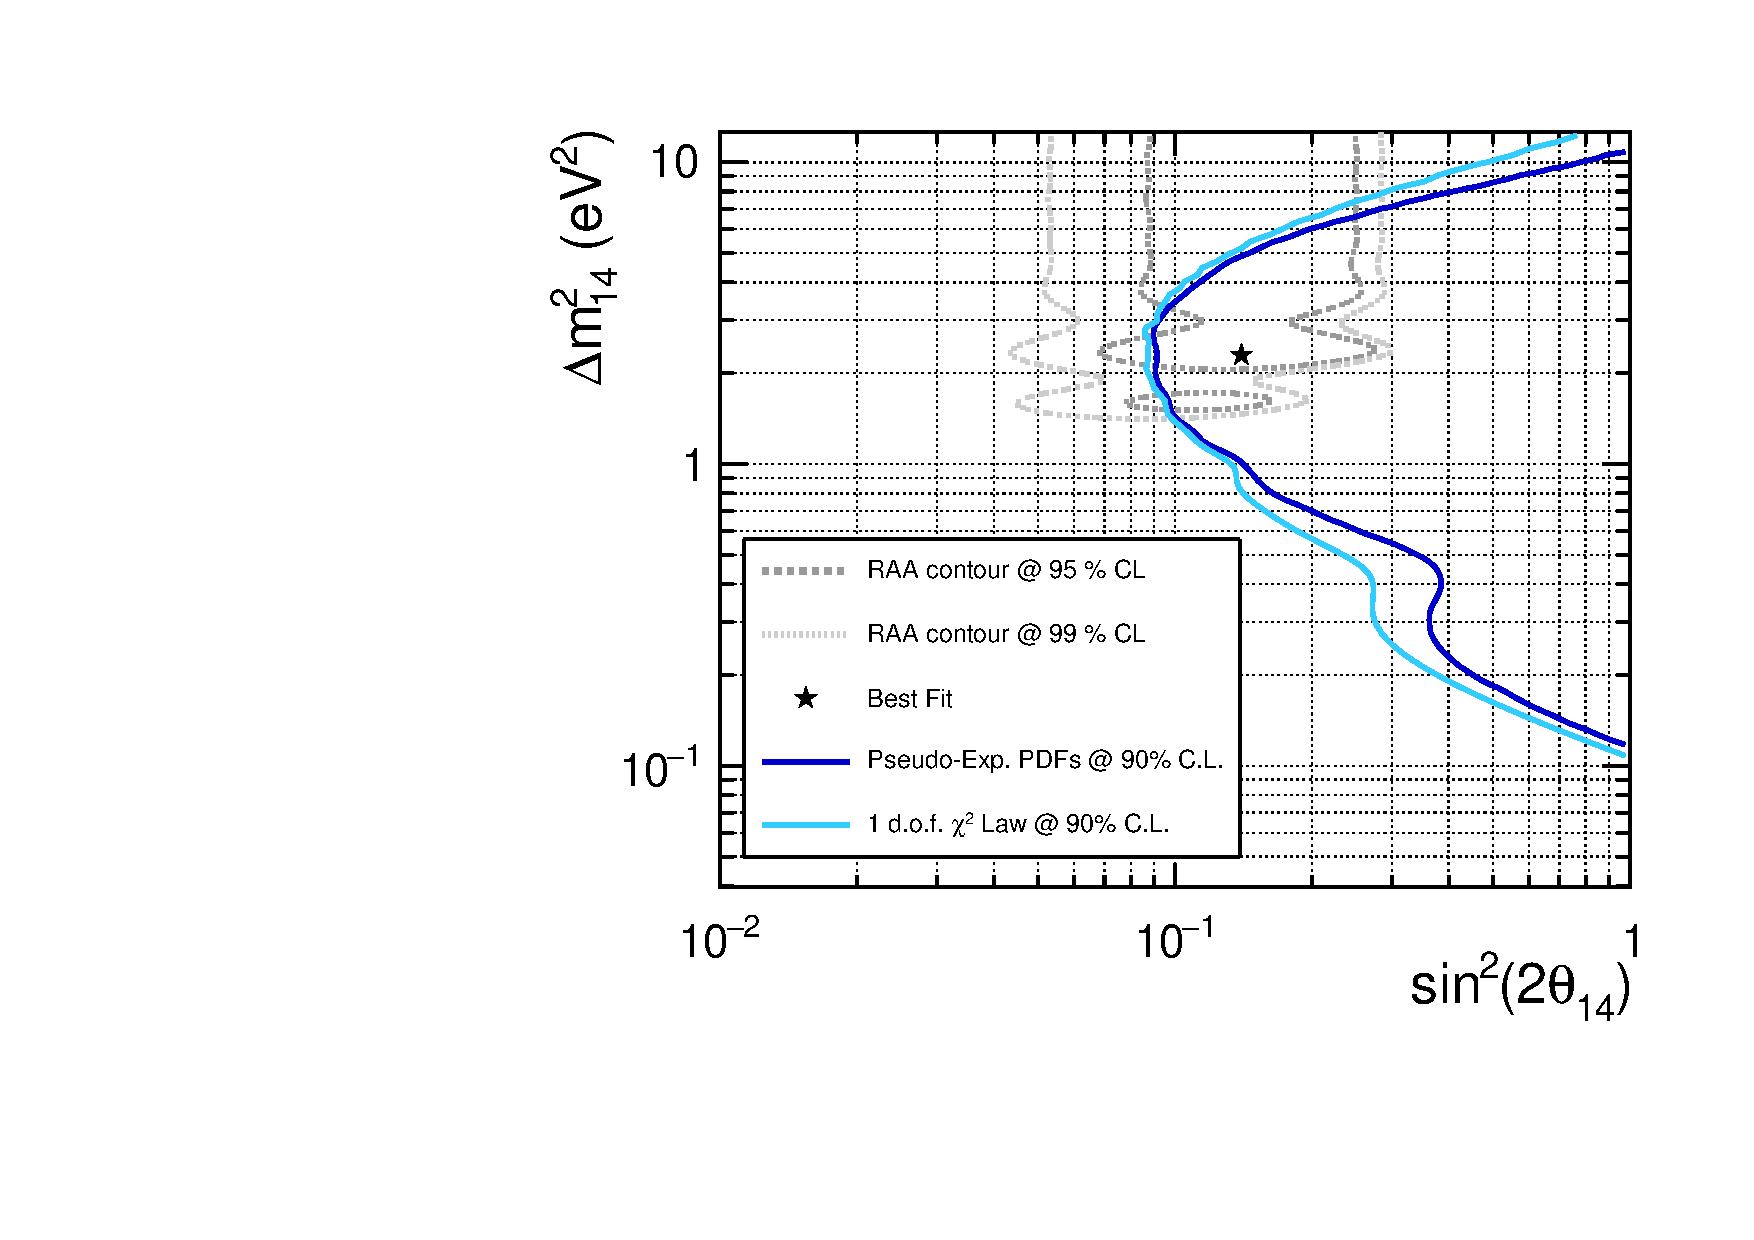
\includegraphics[width=0.92\linewidth]{images/Contours_Raster_PDF_vs_Normal.pdf}
\caption[Contour de sensibilité de l'expérience \textsc{Stereo} en phase 2]{Contour de sensibilité de l'expérience \textsc{Stereo} en phase 2. Le contour en bleu foncé montre la région des paramètres accessibles avec l'inférence statistique issus des véritables PDFs de $\Delta\chi^2$ en \textit{raster-scan}, alors que la ligne cyan montre le contour généré avec les lois normales à un degré de liberté.}
\label{fig:Contours_Raster_PDF_vs_Normal.pdf}

\end{figure}

\begin{figure}[h!]

\centering
\begin{subfigure}[b]{0.49\textwidth}
\centering
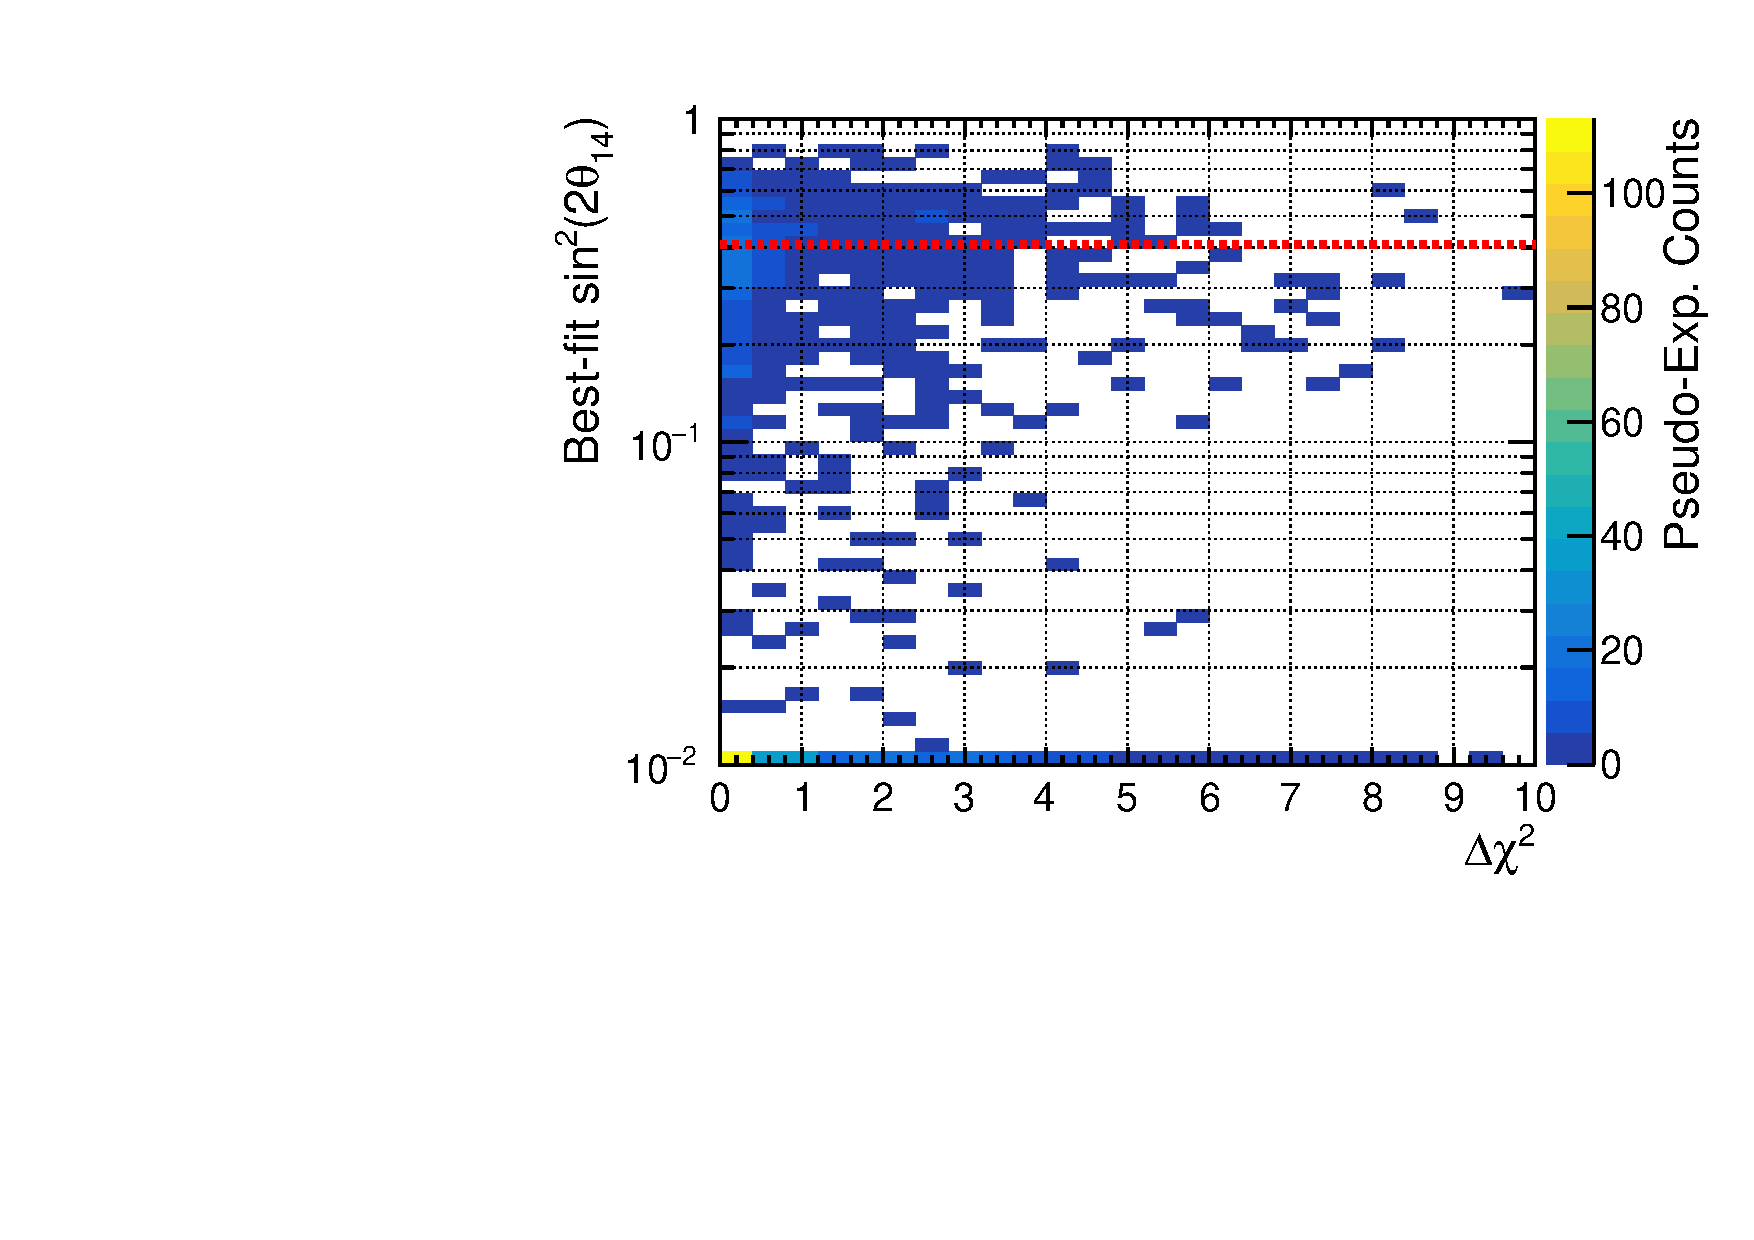
\includegraphics[width=1\linewidth]{images/bestfit_vs_chi2.pdf}
\caption{}
\label{fig:bestfit_vs_chi2.pdf}
\end{subfigure}
~ % attention ! space sensitive
\begin{subfigure}[b]{0.49\textwidth}
\centering
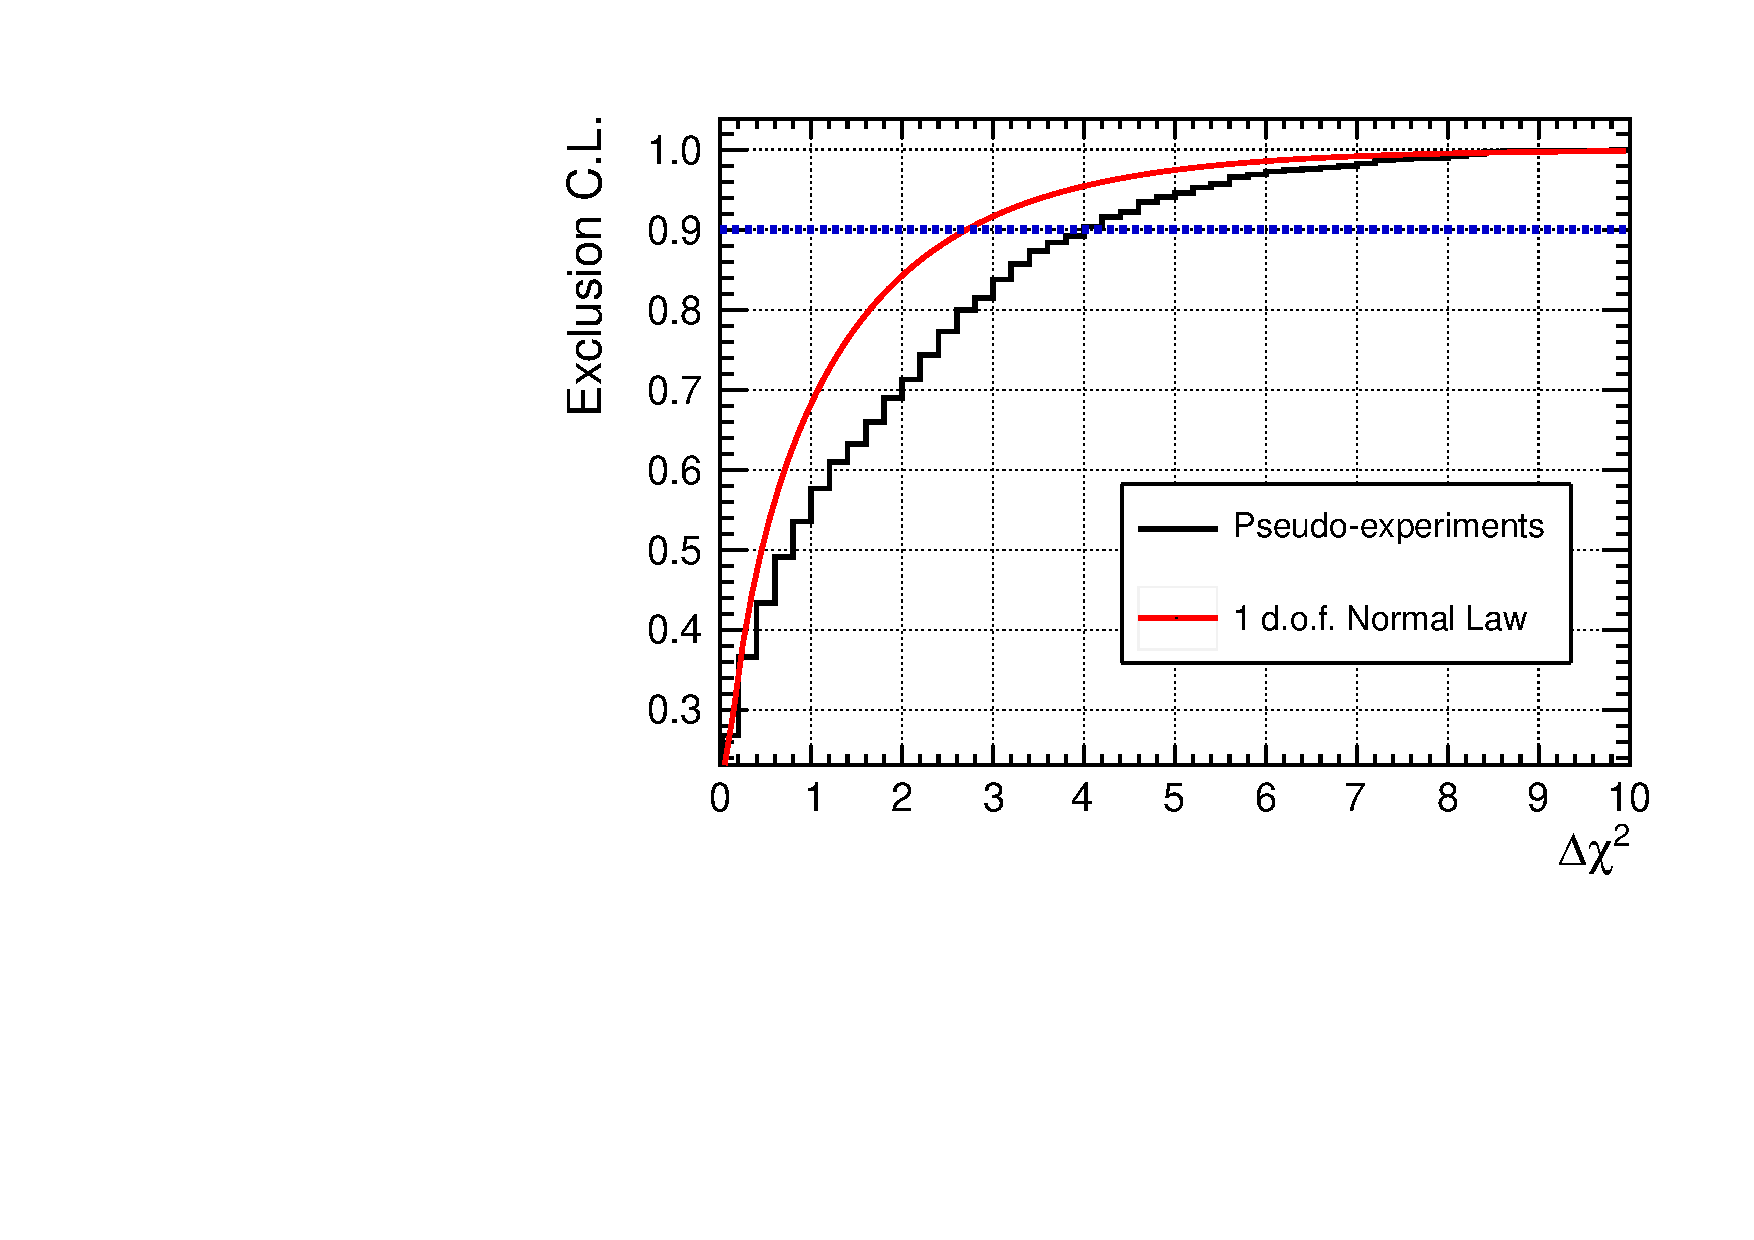
\includegraphics[width=1\linewidth]{images/comparison_cumulative.pdf}
\caption{}
\label{fig:comparison_cumulative.pdf}
\end{subfigure}

\caption[Répartition des \textit{best-fit} en \textit{raster-scan} pour les pseudo-expériences]{Répartition des \textit{best-fit} en \textit{raster-scan} pour les pseudo-expériences. Les pseudo-expériences ont été générées selon l'hypothèse $H_x(\Delta m^2 = \SI{0.25}{eV^2}, \textrm{sin}^2(2\theta) = 0,45)$ représentée par la ligne rouge en pointillé (a). Les \textit{best fit} à bas $\textrm{sin}^2(2\theta)$ ont pour effet d'augmenter la valeur du $\Delta\chi^2$. Cela se répercute sur les contours (b), car pour rejeter une hypothèse $H_x$ à 90 \% C.L. (ligne en pointillés bleue) il faut un $\Delta\chi^2$ plus grand.}
\label{fig:bestfit_vs_deltachi2}
\end{figure}

\clearpage

}

Les courbes de sensibilité sont obtenues en remplaçant les termes $D_{cb}$ par la prédiction non-oscillée $\overline{M}_{cb}$ dans le $\chi^2$. Elles montrent quelles sont les régions de paramètres accessibles avec l'expérience d'après la matrice de covariance présente dans le $\chi^2$. Le volume de réjection est entièrement déterminé par la matrice de covariance.\\

La figure \ref{fig:Contours_Raster_PDF_vs_Normal.pdf} montre le contour de sensibilité pour la phase 2 réalisé en \textit{raster-scan}. On constate que pour les hautes valeurs de $\Delta m^2$ la sensibilité chute. Dans cette région, les motifs d'oscillation sont lavés du fait que la taille de bins devient comparable à celle des oscillations (haut $\Delta m^2 = $ haute fréquence) :

\begin{equation}
    P(\overline{\nu}_e \rightarrow \overline{\nu}_e) = 1 - \left< \textrm{sin}^2\left(\frac{\Delta m^2L}{4E}\right) \right> \textrm{sin}^2(2\theta_{14}) \simeq 1 - \frac{1}{2} \textrm{sin}^2(2\theta_{14}).
\end{equation}

\bigbreak

La probabilité d'oscillation ne dépend plus de la distance de propagation $L$ et donc de la cellule. La variation en $\textrm{sin}^2(2\theta_{14})$ est donc complètement absorbée par les termes  $\phi_b$ dans le $\chi^2$.\\

De manière semblable, la région à bas $\Delta m^2$ n'affecte que les premiers bins en énergie et les distances couvertes par les cellules ne sont pas suffisamment étendues pour que l'expérience soit sensible : les $\phi_b$ absorbent donc la perte de flux à basse énergie.\\

Dans la région $\Delta m^2 \sim \SI{2}{eV^2}$, le déphasage des motifs d'oscillation est suffisant pour que les $\phi_b$ ne puissent assimiler toutes les distorsions: la sensibilité est donc maximale dans cette région. Il est intéressant de noter que les lois normales de $\chi^2$ sont suffisantes pour établir l'inférence statistique, sauf dans les zones où la sensibilité chute : les lois normales surestiment le pouvoir de réjection. Les $\phi_b$ sont responsables de cet écart, mais il est difficile d'interpréter directement leur comportement lors de la génération de pseudo-expériences. En revanche, la position des \textit{best fit} donne des informations pour expliquer cet écart. La figure \ref{fig:bestfit_vs_deltachi2} montre que sur la tranche $\Delta m^2 = \SI{0.25}{eV^2}$, la distribution des $\textrm{sin}^2(2\theta)$ qui minimisent le $\chi^2$ ne suit pas une loi gaussienne centrée sur la valeur injectée $\textrm{sin}^2(2\theta) = 0.45$. En effet, une part importante des \textit{best fit} se trouvent au niveau de l'hypothèse sans neutrino stérile $\textrm{sin}^2(2\theta) = 0$. Ce phénomène a pour effet d'augmenter la valeur $\Delta\chi^2$ des pseudo-expériences, et donc d'atténuer le pouvoir de réjection : il faut un $\Delta\chi^2$ dans les données plus grand pour rejeter l'hypothèse. On retiendra néanmoins que les lois de $\chi^2$ normales suffisent pour décrire le pouvoir de discrimination dans la région pointée par la RAA. Cet aspect est davantage discuté dans la section consacrée à la fusion des résultats obtenus en phase 1 et phase 2 (Section \ref{sec:merge_phases_results}).\\

Bien que les contours de sensibilité donnent un aperçu de l'espace des paramètres accessibles pour tester l'hypothèse du neutrino stérile, les véritables données sont livrées avec des fluctuations statistiques. Les $\Delta\chi^2$ sont affectés et les contours changent. Ce point est présenté dans la section suivante.

\bigbreak


% Puisqu'il s'agit de contours de sensibilité ($D_{cb} \doteq \overline{M}_cb$), le \textit{best fit} est toujours à $\textrm{sin}^2(2\theta) = 0$.

% , et le $\Delta\chi^2$ ne suit plus des lois normales. En effet, lors de la génération de pseudo-expériences, la position du \textit{best fit} en $\textrm{sin}^2(2\theta_{14})$ est altérée par la dépendance du $\chi^2$ en $\phi_b$ et leur distribution n'est plus gaussienne.\\

\subsection{Exemple de contours de réjection}

% peudo_exp_contours.pdf

\afterpage{

\begin{figure}[h!]

\centering
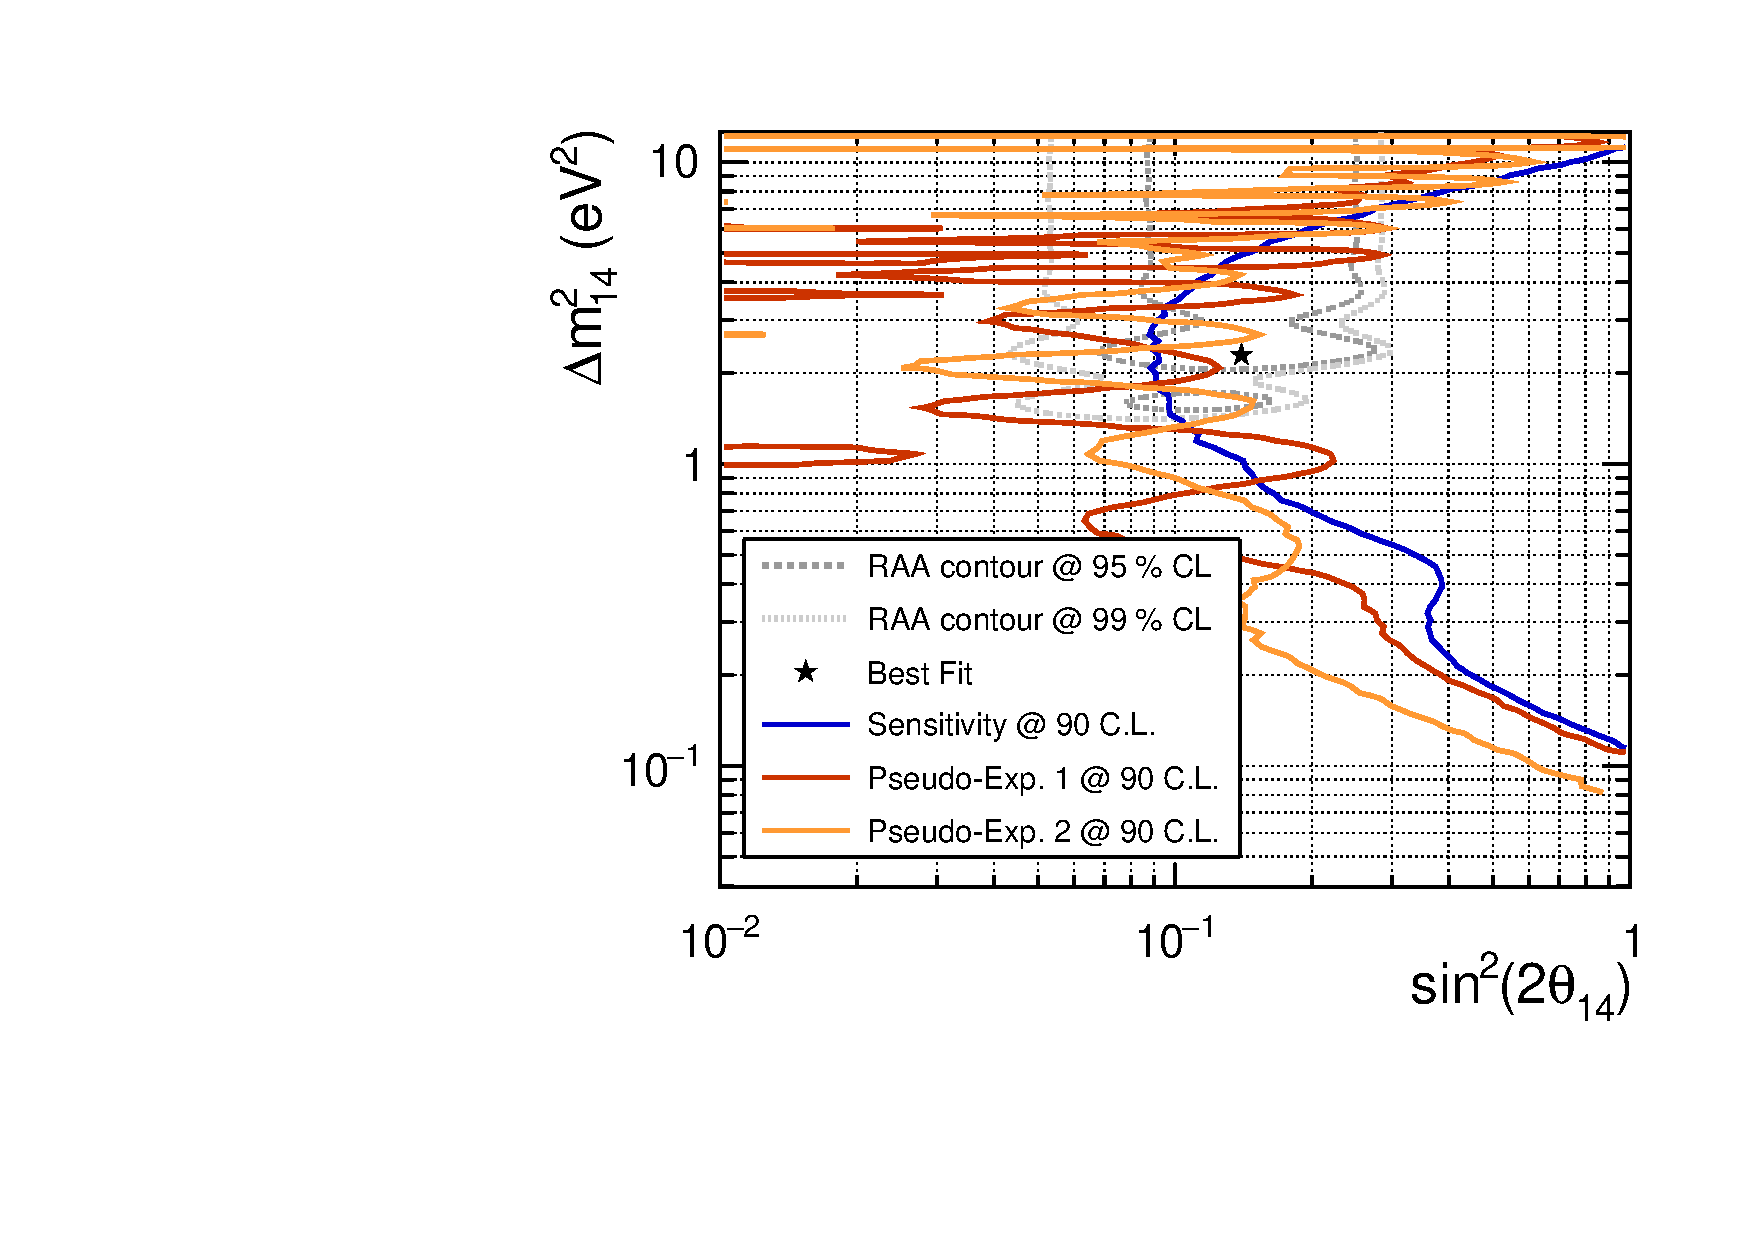
\includegraphics[width=0.74\linewidth]{images/peudo_exp_contours.pdf}
\caption[Comparaison entre les contours de sensibilité et les contours d'exclusion générés par pseudo-expériences]{Comparaison entre les contours de sensibilité et les contours d'exclusion générés par pseudo-expériences (sans neutrino stérile). Ces contours sont générés à partir des cartes de $\Delta\chi^2$ en \textit{raster-scan}. Le contour de sensibilité est dessiné en bleu, tandis que ceux des deux pseudo-expériences sont en rouge et orange. La conversion $\Delta \chi^2 \rightarrow \textit{exclusion C.L.}$ a été établie par pseudo-expériences. La statistique équivalente employée ici est celle des données phase 2 seules.}
\label{fig:peudo_exp_contours.pdf}

\end{figure}

\begin{figure}[h!]

\centering
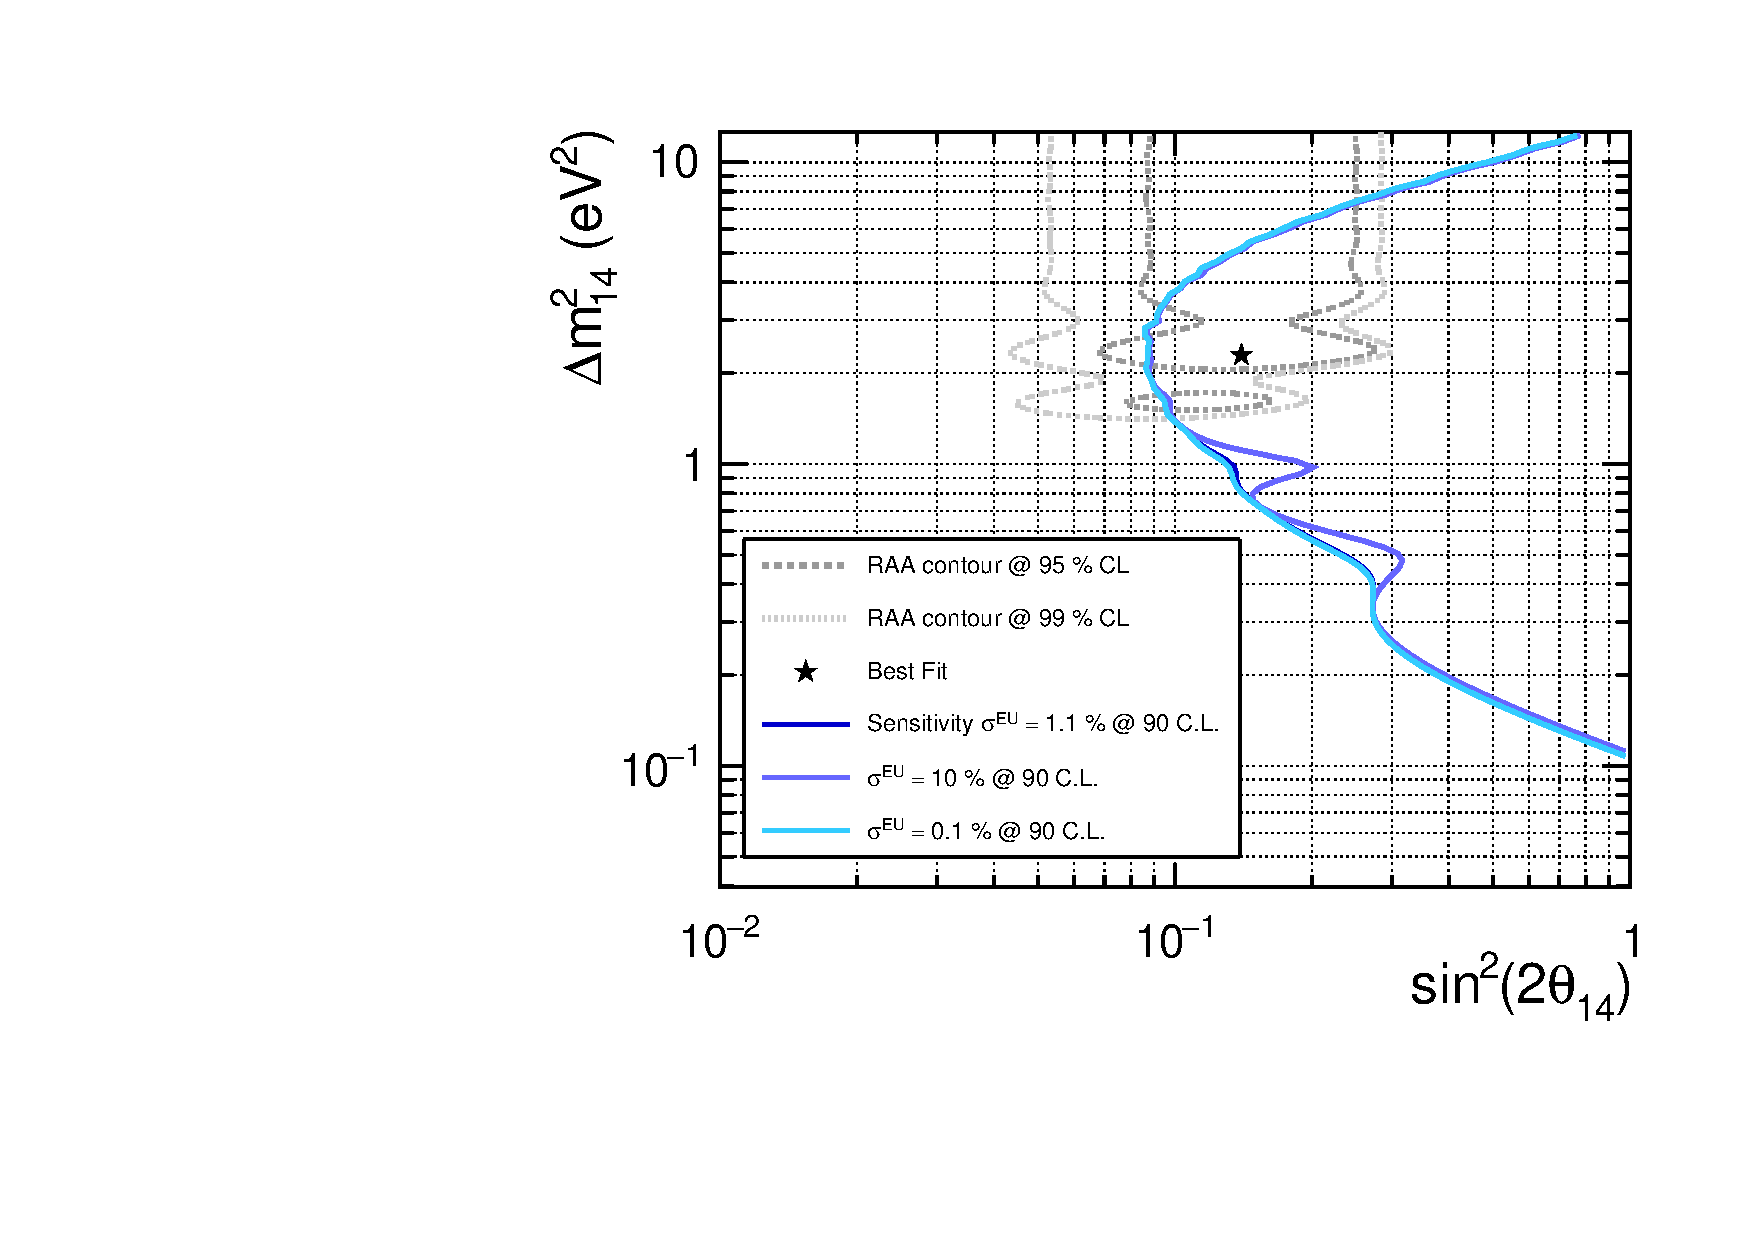
\includegraphics[width=0.74\linewidth]{images/contours_EU.pdf}
\caption[Effet des incertitudes systématiques liées à l'échelle en énergie sur les contours de sensibilité]{Effet des incertitudes systématiques liées à l'échelle en énergie sur les contours de sensibilité. Les contours sont générés avec des lois normales de $\chi^2$ à un degré de liberté. Le contour avec la valeur nominale est dessiné par la courbe bleue foncée.}
\label{fig:contours_EU.pdf}

\clearpage

\end{figure}

\begin{figure}[h!]

\centering
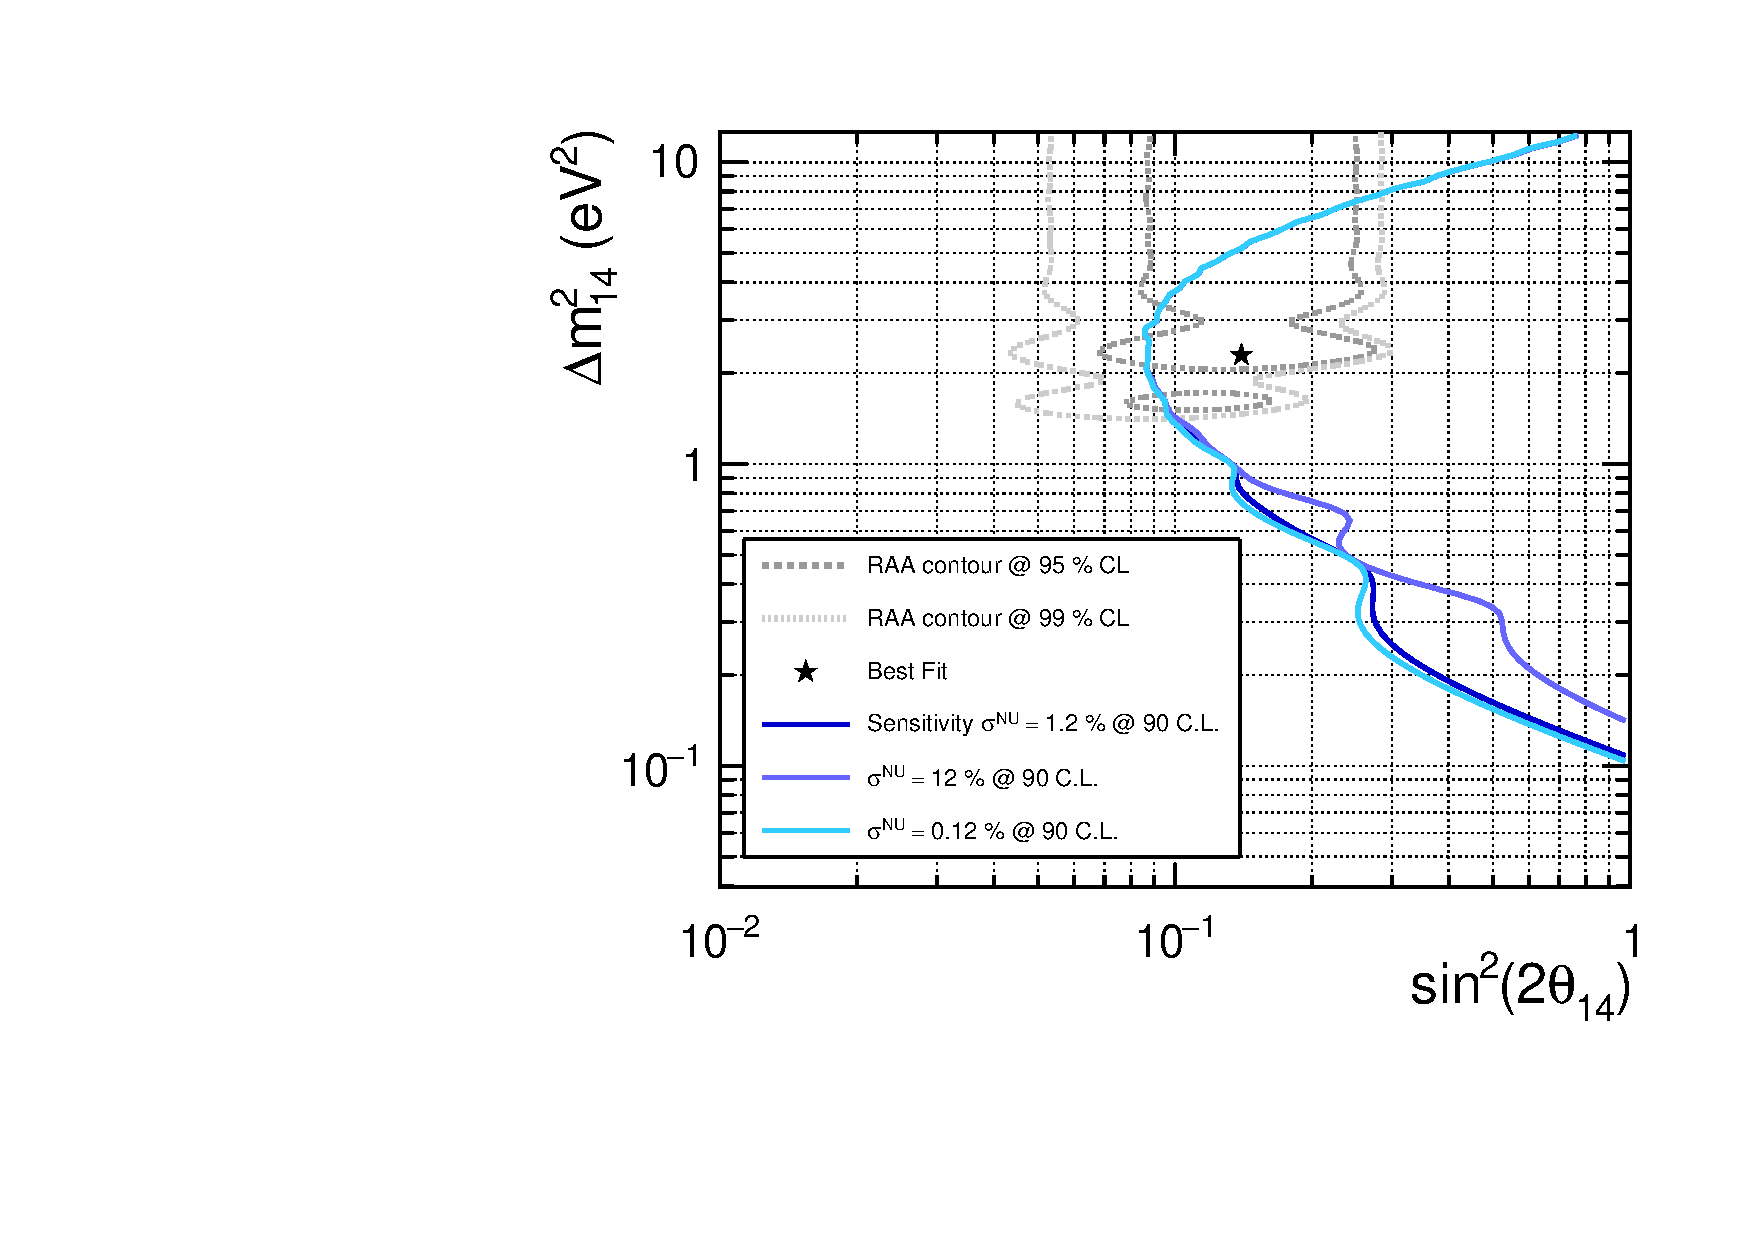
\includegraphics[width=0.78\linewidth]{images/contours_NU.pdf}
\caption[Effet des incertitudes systématiques liées la normalisation relative des cellules sur les contours de sensibilité]{Effet des incertitudes systématiques liées la normalisation relative des cellules sur les contours de sensibilité. Les contours sont générés avec des lois normales de $\chi^2$ à un degré de liberté. Le contour avec la valeur nominale est dessiné par la courbe bleue foncée.}
\label{fig:contours_NU.pdf}

\end{figure}

% contours_global_vs_raster.pdf

\begin{figure}[h!]

\centering
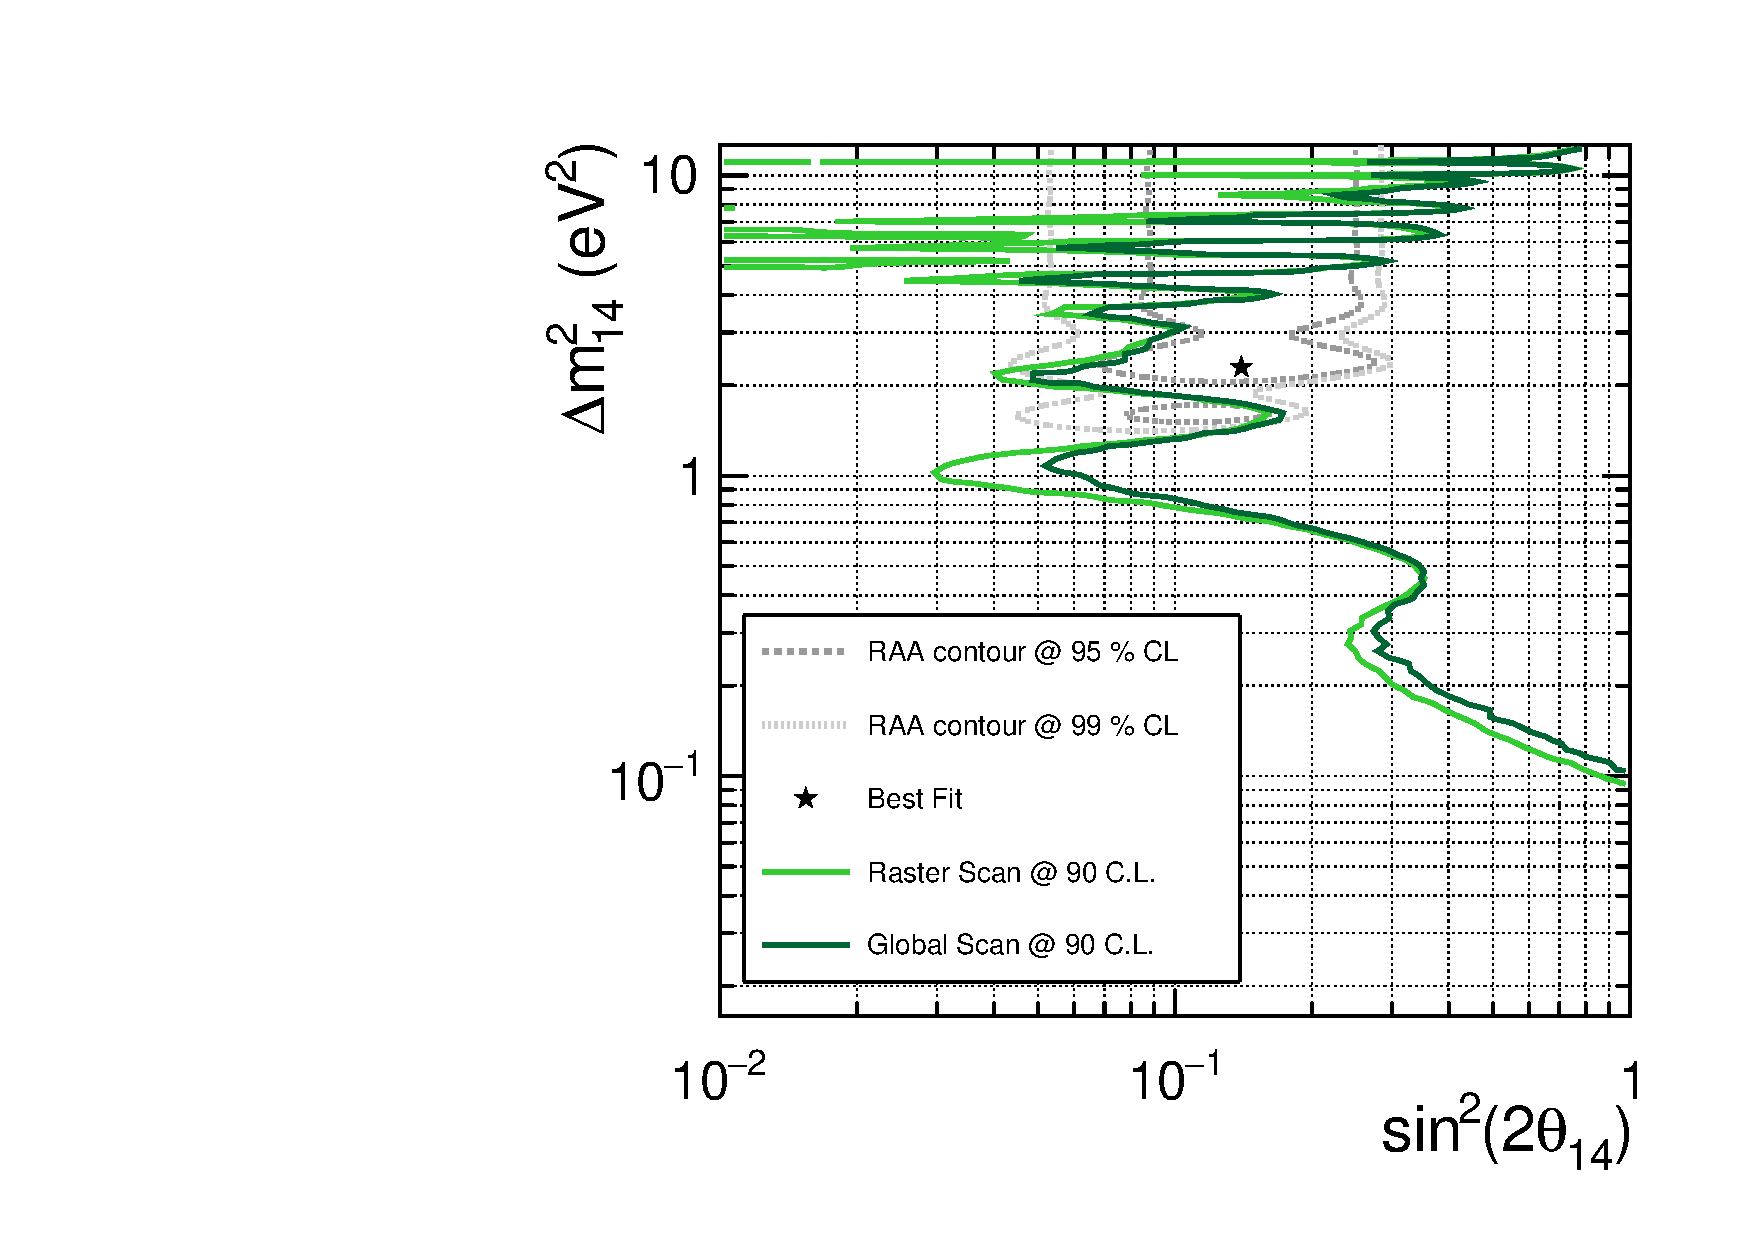
\includegraphics[width=0.78\linewidth]{images/contours_global_vs_raster.pdf}
\caption[Comparaison entre les contours d'exclusion obtenus par \textit{raster-scan} et par \textit{global-scan}]{Comparaison entre les contours d'exclusion obtenus par \textit{raster-scan} et par \textit{global-scan}.}
\label{fig:contours_global_vs_raster.pdf}

\end{figure}

\clearpage

}

Les contours de réjection, ou d'exclusion représentent le sous-espace des paramètres qui est défavorisé par l'expérience avec un certain niveau de confiance. En générant des pseudo-expériences, il est possible de construire des exemples de contours d'exclusion. Ces pseudo-expériences sont fabriquées à partir des données Asimov $\overline{M}_{cb}$ sans neutrino stérile, en tirant des paramètres de nuisance $\alpha$ dans leur gaussienne respective, dont la largeur est dirigée par l'incertitude $\sigma$ :

\begin{equation}
    D_{cb}^* = \overline{M}_{cb}\left(1 + \alpha^{NU}_c\right) + \Delta \eta_{cb}\left(\alpha^{EU}_c + \alpha^{EC}\right) + \alpha^\textrm{stat}_{cb}.
\end{equation}

\bigbreak

Deux contours d'exclusion engendrés par des pseudo-expériences différentes sont superposés avec le contour de sensibilité sur la figure \ref{fig:peudo_exp_contours.pdf}. On pourrait être surpris de constater le comportement ondulatoire des frontières d'exclusion pourtant non présent dans les contours de sensibilité. Certains motifs d'oscillation en $\Delta m^2$ peuvent imiter l'allure des fluctuations statistiques. Dans ce cas, la valeur du $\chi^2$ est réduite et le pouvoir de réjection est amoindri. Ce phénomène provoque des \og creux \fg{} de sensibilité. \textit{A contrario}, lorsque les fluctuations statistiques se retrouvent en opposition de phase avec la forme de la distorsion en $\Delta m^2$, la sensibilité est accrue. Finalement, l'aspect périodique de ces pics de sensibilité s'explique par la nature des déformations induites par le paramètre $\Delta m_{14}^2$. En effet $\Delta m_{14}^2$ conduit la fréquence des oscillations, donc à chaque harmonique les fluctuations peuvent correspondre à nouveau avec le modèle. L'amplitude et la phase de ces \og peignes \fg{} dépendent de la définition de chaque bin en énergie et de la position des cellules par rapport au c\oe ur du réacteur. En appliquant l'extraction des taux de comptage neutrino avec un déphasage de la moitié de la largeur des bins, les vagues changeraient de position et d'amplitude. Cet effet pourrait être atténué en moyennant plusieurs contours de réjection réalisés avec différents binnings.\\

Les lignes d'exclusion serpentent autour du contour de sensibilité, car les fluctuations sur $M_{cb}$ sont appliquées à partir de la valeur centrale $\overline{M}_{cb}$. On remarque cependant quelques zones à bas $\textrm{sin}^2(2\theta)$ qui sont exclues dans certaines tranches en $\Delta m^2$, suggérant le rejet de l'hypothèse nulle. Il s'agit d'un artéfact de l'inférence en \textit{raster-scan}. Pour ces $\Delta m^2$, le \textit{best fit} se trouve en un scénario en $\textrm{sin}^2(2\theta)$ placé entre les deux zones rejetées, et le $\chi^2$ est suffisamment faible pour rejeter les faibles angles de mélange alors que les pseudo-expériences ont été générées à partir du modèle non-oscillé. Ces zones n'ont pas de signification physique, c'est pourquoi elles sont ignorées pour la publication des résultats. Afin de débarrasser de ces signaux faux-positifs, il est nécessaire de considérer l'analyse statistique en \textit{global-scan} : un exemple est discuté dans la Section \ref{sec:global_scan_example}.


\bigbreak

\subsection{Impact des systématiques sur les contours}

Dans la Section \ref{seq:incert_propag} il a été conclu que les incertitudes statistiques étaient dominantes face aux systématiques avec $\chi^2_\phi$. Cet aspect se traduit aussi dans les contours de sensibilités. Pour observer l'effet des erreurs systématiques sur le pouvoir de réjection de \textsc{Stereo}, chaque systématique a individuellement été multipliée ou divisée par 10. Les résultats sont présentés sur les Figures \ref{fig:contours_EU.pdf} et \ref{fig:contours_NU.pdf}. Lorsque l'incertitude sur l'échelle en énergie (EU) est augmentée d'un facteur 10, seule la partie à bas $\Delta m^2$ est légèrement affectée. En particulier, les pertes de sensibilité sont localisées autour de tranches à $\Delta m^2 \sim \SI{1}{eV^2}$ et  $\Delta m^2 \sim \SI{0.5}{eV^2}$. Pour comprendre la position de ces spots, il faudrait analyser la corrélation entre les motifs d'oscillation binnés et la nature des déformations induites par les incertitudes sur l'échelle énergie. La forme des distribution en $\Delta \eta_{cb}$ ainsi que la valeur des \textit{pull terms} ajustés (avec formalisme en $\chi^2_\phi$ adéquat) seraient en mesure de donner plus d'informations à ce sujet. En revanche, lorsque les erreurs sur l'échelle en énergie sont réduites d'un facteur 10, aucun effet n'est notable. Pour comprendre cet effet, il faut rappeler que les déformations induites par $\alpha^{EU}$ sont proportionnelles à $\eta_{cb}$ qui dépendent du binning en énergie : plus le binning est fin, plus les transferts bin à bin sont importants. La sensibilité est donc en partie limitée par la taille des bins en énergie qui a été contrainte avec les procédures d'extraction des spectres neutrinos (cf. Section \ref{sec:nu_extraction}).\\

En amplifiant les erreurs systématiques sur la normalisation relative des cellules (NU), la figure \ref{fig:contours_NU.pdf} montre aussi que seule la partie à bas $\Delta m^2$ ($< \SI{1}{eV^2}$) est sensible à ce paramètre. À haut $\Delta m^2$ (haute fréquence) les distorsions dues à l'oscillation se répercutent sur la forme des spectres de chaque cellule, alors qu'à basse fréquence le développement de l'oscillation n'est visible que par un effet de normalisation relative entre les cellules. De fait, une grande imprécision sur $NU$ désamorce la capacité de discriminer une oscillation à bas $\Delta m^2$ d'un effet systématique. En revanche, le gain de sensibilité en divisant les erreurs systématiques par 10 est minime. En effet, pour $\Delta m^2 < \SI{1}{eV^2}$  l'écroulement du contour est à la fois causé par les $\phi_b$ qui ont la possibilité de combler la perte de flux à basse énergie, et les erreurs statistiques. Améliorer la connaissance de la normalisation relative n'accorderait donc pas une meilleure couverture pour l'analyse avec $\chi^2_\phi$.

\bigbreak

\subsection{Contours en global-scan}
\label{sec:global_scan_example}

L'analyse en \textit{global-scan} constitue l'inférence ultime pour dessiner les contours d'exclusion. La difficulté principale dans l'emploi de cette méthode réside dans la génération des PDFs en $\Delta \chi^2$. L'exemple présenté sur la figure \ref{fig:contours_global_vs_raster.pdf} a été réalisé avec 500 pseudo-expériences pour chaque point de la grille en $(\Delta m^2, \textrm{sin}^2(2\theta))$ (100x100). Puisque la nature du problème empêche l'utilisation de minimiseurs par gradient, la recherche du \textit{best fit} est faite manuellement en testant chaque trame en $\Delta m^2$. Cet aspect ne pourra être optimisé à l'avenir, cependant la minimisation en $\textrm{sin}^2(2\theta)$ pourra être revue pour un gain de performances non négligeables.\\

Comme il a été mentionné précédemment, le \textit{global-scan} permet de déduire la probabilité d'un scénario particulier en $\Delta m^2$. La comparaison avec le \textit{raster-scan} de la figure \ref{fig:peudo_exp_contours.pdf} montre que l'analyse en \textit{global-scan} s'est débarrassée des zones d'exclusion à basse amplitude d'oscillation. L'amplitude des vagues formées par le contour est aussi réduite de manière générale. En définitive cette étude nous apprend que les contours générés en \textit{raster-scan} surestiment légèrement le pouvoir de discrimination en $\textrm{sin}^2(2\theta)$ d'une expérience. Il est donc important de garder à l'esprit qu'il n'est pas pertinent de discuter les résultats des expériences neutrino autour du trait lorsque ceux-ci sont générés en \textit{raster-scan}.

\bigbreak

% TODO FM : Conclusion ch6


%\subsection{Combinaison des deux phases}
%\label{sec:phases_comb_sensitivity}

